\documentclass[twoside]{book}

% Packages required by doxygen
\usepackage{fixltx2e}
\usepackage{calc}
\usepackage{doxygen}
\usepackage[export]{adjustbox} % also loads graphicx
\usepackage{graphicx}
\usepackage[utf8]{inputenc}
\usepackage{makeidx}
\usepackage{multicol}
\usepackage{multirow}
\PassOptionsToPackage{warn}{textcomp}
\usepackage{textcomp}
\usepackage[nointegrals]{wasysym}
\usepackage[table]{xcolor}

% Font selection
\usepackage[T1]{fontenc}
\usepackage[scaled=.90]{helvet}
\usepackage{courier}
\usepackage{amssymb}
\usepackage{sectsty}
\renewcommand{\familydefault}{\sfdefault}
\allsectionsfont{%
  \fontseries{bc}\selectfont%
  \color{darkgray}%
}
\renewcommand{\DoxyLabelFont}{%
  \fontseries{bc}\selectfont%
  \color{darkgray}%
}
\newcommand{\+}{\discretionary{\mbox{\scriptsize$\hookleftarrow$}}{}{}}

% Page & text layout
\usepackage{geometry}
\geometry{%
  a4paper,%
  top=2.5cm,%
  bottom=2.5cm,%
  left=2.5cm,%
  right=2.5cm%
}
\tolerance=750
\hfuzz=15pt
\hbadness=750
\setlength{\emergencystretch}{15pt}
\setlength{\parindent}{0cm}
\setlength{\parskip}{3ex plus 2ex minus 2ex}
\makeatletter
\renewcommand{\paragraph}{%
  \@startsection{paragraph}{4}{0ex}{-1.0ex}{1.0ex}{%
    \normalfont\normalsize\bfseries\SS@parafont%
  }%
}
\renewcommand{\subparagraph}{%
  \@startsection{subparagraph}{5}{0ex}{-1.0ex}{1.0ex}{%
    \normalfont\normalsize\bfseries\SS@subparafont%
  }%
}
\makeatother

% Headers & footers
\usepackage{fancyhdr}
\pagestyle{fancyplain}
\fancyhead[LE]{\fancyplain{}{\bfseries\thepage}}
\fancyhead[CE]{\fancyplain{}{}}
\fancyhead[RE]{\fancyplain{}{\bfseries\leftmark}}
\fancyhead[LO]{\fancyplain{}{\bfseries\rightmark}}
\fancyhead[CO]{\fancyplain{}{}}
\fancyhead[RO]{\fancyplain{}{\bfseries\thepage}}
\fancyfoot[LE]{\fancyplain{}{}}
\fancyfoot[CE]{\fancyplain{}{}}
\fancyfoot[RE]{\fancyplain{}{\bfseries\scriptsize Generated by Doxygen }}
\fancyfoot[LO]{\fancyplain{}{\bfseries\scriptsize Generated by Doxygen }}
\fancyfoot[CO]{\fancyplain{}{}}
\fancyfoot[RO]{\fancyplain{}{}}
\renewcommand{\footrulewidth}{0.4pt}
\renewcommand{\chaptermark}[1]{%
  \markboth{#1}{}%
}
\renewcommand{\sectionmark}[1]{%
  \markright{\thesection\ #1}%
}

% Indices & bibliography
\usepackage{natbib}
\usepackage[titles]{tocloft}
\setcounter{tocdepth}{3}
\setcounter{secnumdepth}{5}
\makeindex

% Hyperlinks (required, but should be loaded last)
\usepackage{ifpdf}
\ifpdf
  \usepackage[pdftex,pagebackref=true]{hyperref}
\else
  \usepackage[ps2pdf,pagebackref=true]{hyperref}
\fi
\hypersetup{%
  colorlinks=true,%
  linkcolor=blue,%
  citecolor=blue,%
  unicode%
}

% Custom commands
\newcommand{\clearemptydoublepage}{%
  \newpage{\pagestyle{empty}\cleardoublepage}%
}

\usepackage{caption}
\captionsetup{labelsep=space,justification=centering,font={bf},singlelinecheck=off,skip=4pt,position=top}

%===== C O N T E N T S =====

\begin{document}

% Titlepage & ToC
\hypersetup{pageanchor=false,
             bookmarksnumbered=true,
             pdfencoding=unicode
            }
\pagenumbering{alph}
\begin{titlepage}
\vspace*{7cm}
\begin{center}%
{\Large Noob Engine }\\
\vspace*{1cm}
{\large Generated by Doxygen 1.8.13}\\
\end{center}
\end{titlepage}
\clearemptydoublepage
\pagenumbering{roman}
\tableofcontents
\clearemptydoublepage
\pagenumbering{arabic}
\hypersetup{pageanchor=true}

%--- Begin generated contents ---
\chapter{Namespace Index}
\section{Namespace List}
Here is a list of all namespaces with brief descriptions\+:\begin{DoxyCompactList}
\item\contentsline{section}{\hyperlink{namespaceCam}{Cam} }{\pageref{namespaceCam}}{}
\item\contentsline{section}{\hyperlink{namespaceControl}{Control} }{\pageref{namespaceControl}}{}
\end{DoxyCompactList}

\chapter{Hierarchical Index}
\section{Class Hierarchy}
This inheritance list is sorted roughly, but not completely, alphabetically\+:\begin{DoxyCompactList}
\item \contentsline{section}{Camera}{\pageref{classCamera}}{}
\item \contentsline{section}{Controller}{\pageref{classController}}{}
\item \contentsline{section}{Hitbox}{\pageref{classHitbox}}{}
\item \contentsline{section}{Instance3D}{\pageref{classInstance3D}}{}
\item \contentsline{section}{Object}{\pageref{classObject}}{}
\begin{DoxyCompactList}
\item \contentsline{section}{Base}{\pageref{classBase}}{}
\item \contentsline{section}{Cube}{\pageref{classCube}}{}
\item \contentsline{section}{Pave}{\pageref{classPave}}{}
\item \contentsline{section}{Skybox}{\pageref{classSkybox}}{}
\end{DoxyCompactList}
\item \contentsline{section}{Scene}{\pageref{classScene}}{}
\end{DoxyCompactList}

\chapter{Class Index}
\section{Class List}
Here are the classes, structs, unions and interfaces with brief descriptions\+:\begin{DoxyCompactList}
\item\contentsline{section}{\hyperlink{classBase}{Base} }{\pageref{classBase}}{}
\item\contentsline{section}{\hyperlink{classCamera}{Camera} }{\pageref{classCamera}}{}
\item\contentsline{section}{\hyperlink{classController}{Controller} }{\pageref{classController}}{}
\item\contentsline{section}{\hyperlink{classCube}{Cube} }{\pageref{classCube}}{}
\item\contentsline{section}{\hyperlink{classHitbox}{Hitbox} }{\pageref{classHitbox}}{}
\item\contentsline{section}{\hyperlink{classInstance3D}{Instance3D} }{\pageref{classInstance3D}}{}
\item\contentsline{section}{\hyperlink{classObject}{Object} }{\pageref{classObject}}{}
\item\contentsline{section}{\hyperlink{classPave}{Pave} }{\pageref{classPave}}{}
\item\contentsline{section}{\hyperlink{classScene}{Scene} }{\pageref{classScene}}{}
\item\contentsline{section}{\hyperlink{classSkybox}{Skybox} }{\pageref{classSkybox}}{}
\end{DoxyCompactList}

\chapter{File Index}
\section{File List}
Here is a list of all files with brief descriptions\+:\begin{DoxyCompactList}
\item\contentsline{section}{include/\hyperlink{base_8h}{base.\+h} }{\pageref{base_8h}}{}
\item\contentsline{section}{include/\hyperlink{camera_8h}{camera.\+h} }{\pageref{camera_8h}}{}
\item\contentsline{section}{include/\hyperlink{controller_8h}{controller.\+h} }{\pageref{controller_8h}}{}
\item\contentsline{section}{include/\hyperlink{cube_8h}{cube.\+h} }{\pageref{cube_8h}}{}
\item\contentsline{section}{include/\hyperlink{debugger_8h}{debugger.\+h} }{\pageref{debugger_8h}}{}
\item\contentsline{section}{include/\hyperlink{hitbox_8h}{hitbox.\+h} }{\pageref{hitbox_8h}}{}
\item\contentsline{section}{include/\hyperlink{instance3D_8h}{instance3\+D.\+h} }{\pageref{instance3D_8h}}{}
\item\contentsline{section}{include/\hyperlink{object_8h}{object.\+h} }{\pageref{object_8h}}{}
\item\contentsline{section}{include/\hyperlink{pave_8h}{pave.\+h} }{\pageref{pave_8h}}{}
\item\contentsline{section}{include/\hyperlink{scene_8h}{scene.\+h} }{\pageref{scene_8h}}{}
\item\contentsline{section}{include/\hyperlink{skybox_8h}{skybox.\+h} }{\pageref{skybox_8h}}{}
\item\contentsline{section}{scripts/\hyperlink{main_8cpp}{main.\+cpp} }{\pageref{main_8cpp}}{}
\item\contentsline{section}{src/\hyperlink{base_8cpp}{base.\+cpp} }{\pageref{base_8cpp}}{}
\item\contentsline{section}{src/\hyperlink{camera_8cpp}{camera.\+cpp} }{\pageref{camera_8cpp}}{}
\item\contentsline{section}{src/\hyperlink{controller_8cpp}{controller.\+cpp} }{\pageref{controller_8cpp}}{}
\item\contentsline{section}{src/\hyperlink{cube_8cpp}{cube.\+cpp} }{\pageref{cube_8cpp}}{}
\item\contentsline{section}{src/\hyperlink{hitbox_8cpp}{hitbox.\+cpp} }{\pageref{hitbox_8cpp}}{}
\item\contentsline{section}{src/\hyperlink{pave_8cpp}{pave.\+cpp} }{\pageref{pave_8cpp}}{}
\item\contentsline{section}{src/\hyperlink{scene_8cpp}{scene.\+cpp} }{\pageref{scene_8cpp}}{}
\item\contentsline{section}{src/\hyperlink{skybox_8cpp}{skybox.\+cpp} }{\pageref{skybox_8cpp}}{}
\end{DoxyCompactList}

\chapter{Namespace Documentation}
\hypertarget{namespaceCam}{}\section{Cam Namespace Reference}
\label{namespaceCam}\index{Cam@{Cam}}
\subsection*{Variables}
\begin{DoxyCompactItemize}
\item 
constexpr float \hyperlink{namespaceCam_a19ee86132ca8219870515f550db61f93}{Y\+AW} = -\/90.\+0f
\item 
constexpr float \hyperlink{namespaceCam_a5ba61b0ad0aa42c7887436a7f0ac5628}{P\+I\+T\+CH} = 0.\+0f
\item 
constexpr float \hyperlink{namespaceCam_a9827a53b18675bb2e3845aadd51e476e}{S\+P\+E\+ED} = 20.f
\item 
constexpr float \hyperlink{namespaceCam_a3d86110004c8f438362c6a86532efe9c}{S\+E\+N\+S\+I\+T\+I\+V\+I\+TY} = 0.\+1f
\item 
constexpr float \hyperlink{namespaceCam_a44d3e32060d4c50bb27d7110c754cb69}{Z\+O\+OM} = 45.\+0f
\item 
constexpr float \hyperlink{namespaceCam_a73d39e25ed690e5a0ea871fb939d9e4d}{N\+E\+AR} = 0.\+1f
\item 
constexpr float \hyperlink{namespaceCam_a469e970813928ea23b912618d3401368}{F\+AR} = 1000.\+0f
\end{DoxyCompactItemize}


\subsection{Variable Documentation}
\mbox{\Hypertarget{namespaceCam_a469e970813928ea23b912618d3401368}\label{namespaceCam_a469e970813928ea23b912618d3401368}} 
\index{Cam@{Cam}!F\+AR@{F\+AR}}
\index{F\+AR@{F\+AR}!Cam@{Cam}}
\subsubsection{\texorpdfstring{F\+AR}{FAR}}
{\footnotesize\ttfamily constexpr float Cam\+::\+F\+AR = 1000.\+0f}

\mbox{\Hypertarget{namespaceCam_a73d39e25ed690e5a0ea871fb939d9e4d}\label{namespaceCam_a73d39e25ed690e5a0ea871fb939d9e4d}} 
\index{Cam@{Cam}!N\+E\+AR@{N\+E\+AR}}
\index{N\+E\+AR@{N\+E\+AR}!Cam@{Cam}}
\subsubsection{\texorpdfstring{N\+E\+AR}{NEAR}}
{\footnotesize\ttfamily constexpr float Cam\+::\+N\+E\+AR = 0.\+1f}

\mbox{\Hypertarget{namespaceCam_a5ba61b0ad0aa42c7887436a7f0ac5628}\label{namespaceCam_a5ba61b0ad0aa42c7887436a7f0ac5628}} 
\index{Cam@{Cam}!P\+I\+T\+CH@{P\+I\+T\+CH}}
\index{P\+I\+T\+CH@{P\+I\+T\+CH}!Cam@{Cam}}
\subsubsection{\texorpdfstring{P\+I\+T\+CH}{PITCH}}
{\footnotesize\ttfamily constexpr float Cam\+::\+P\+I\+T\+CH = 0.\+0f}

\mbox{\Hypertarget{namespaceCam_a3d86110004c8f438362c6a86532efe9c}\label{namespaceCam_a3d86110004c8f438362c6a86532efe9c}} 
\index{Cam@{Cam}!S\+E\+N\+S\+I\+T\+I\+V\+I\+TY@{S\+E\+N\+S\+I\+T\+I\+V\+I\+TY}}
\index{S\+E\+N\+S\+I\+T\+I\+V\+I\+TY@{S\+E\+N\+S\+I\+T\+I\+V\+I\+TY}!Cam@{Cam}}
\subsubsection{\texorpdfstring{S\+E\+N\+S\+I\+T\+I\+V\+I\+TY}{SENSITIVITY}}
{\footnotesize\ttfamily constexpr float Cam\+::\+S\+E\+N\+S\+I\+T\+I\+V\+I\+TY = 0.\+1f}

\mbox{\Hypertarget{namespaceCam_a9827a53b18675bb2e3845aadd51e476e}\label{namespaceCam_a9827a53b18675bb2e3845aadd51e476e}} 
\index{Cam@{Cam}!S\+P\+E\+ED@{S\+P\+E\+ED}}
\index{S\+P\+E\+ED@{S\+P\+E\+ED}!Cam@{Cam}}
\subsubsection{\texorpdfstring{S\+P\+E\+ED}{SPEED}}
{\footnotesize\ttfamily constexpr float Cam\+::\+S\+P\+E\+ED = 20.f}

\mbox{\Hypertarget{namespaceCam_a19ee86132ca8219870515f550db61f93}\label{namespaceCam_a19ee86132ca8219870515f550db61f93}} 
\index{Cam@{Cam}!Y\+AW@{Y\+AW}}
\index{Y\+AW@{Y\+AW}!Cam@{Cam}}
\subsubsection{\texorpdfstring{Y\+AW}{YAW}}
{\footnotesize\ttfamily constexpr float Cam\+::\+Y\+AW = -\/90.\+0f}

\mbox{\Hypertarget{namespaceCam_a44d3e32060d4c50bb27d7110c754cb69}\label{namespaceCam_a44d3e32060d4c50bb27d7110c754cb69}} 
\index{Cam@{Cam}!Z\+O\+OM@{Z\+O\+OM}}
\index{Z\+O\+OM@{Z\+O\+OM}!Cam@{Cam}}
\subsubsection{\texorpdfstring{Z\+O\+OM}{ZOOM}}
{\footnotesize\ttfamily constexpr float Cam\+::\+Z\+O\+OM = 45.\+0f}


\hypertarget{namespaceControl}{}\section{Control Namespace Reference}
\label{namespaceControl}\index{Control@{Control}}
\subsection*{Variables}
\begin{DoxyCompactItemize}
\item 
constexpr float \hyperlink{namespaceControl_a56babc87b3c7df1aba525ccd3e80abf7}{S\+P\+E\+ED} = 0.\+01f
\item 
constexpr float \hyperlink{namespaceControl_a04a945fadad95f496ca4e1f3d870881a}{J\+U\+MP} = 0.\+01f
\end{DoxyCompactItemize}


\subsection{Variable Documentation}
\mbox{\Hypertarget{namespaceControl_a04a945fadad95f496ca4e1f3d870881a}\label{namespaceControl_a04a945fadad95f496ca4e1f3d870881a}} 
\index{Control@{Control}!J\+U\+MP@{J\+U\+MP}}
\index{J\+U\+MP@{J\+U\+MP}!Control@{Control}}
\subsubsection{\texorpdfstring{J\+U\+MP}{JUMP}}
{\footnotesize\ttfamily constexpr float Control\+::\+J\+U\+MP = 0.\+01f}

\mbox{\Hypertarget{namespaceControl_a56babc87b3c7df1aba525ccd3e80abf7}\label{namespaceControl_a56babc87b3c7df1aba525ccd3e80abf7}} 
\index{Control@{Control}!S\+P\+E\+ED@{S\+P\+E\+ED}}
\index{S\+P\+E\+ED@{S\+P\+E\+ED}!Control@{Control}}
\subsubsection{\texorpdfstring{S\+P\+E\+ED}{SPEED}}
{\footnotesize\ttfamily constexpr float Control\+::\+S\+P\+E\+ED = 0.\+01f}


\chapter{Class Documentation}
\hypertarget{classBase}{}\section{Base Class Reference}
\label{classBase}\index{Base@{Base}}


{\ttfamily \#include $<$base.\+h$>$}



Inheritance diagram for Base\+:\nopagebreak
\begin{figure}[H]
\begin{center}
\leavevmode
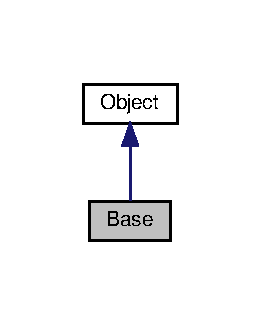
\includegraphics[width=125pt]{classBase__inherit__graph}
\end{center}
\end{figure}


Collaboration diagram for Base\+:\nopagebreak
\begin{figure}[H]
\begin{center}
\leavevmode
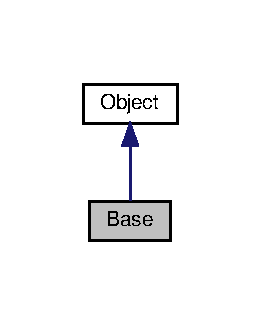
\includegraphics[width=125pt]{classBase__coll__graph}
\end{center}
\end{figure}
\subsection*{Public Member Functions}
\begin{DoxyCompactItemize}
\item 
\hyperlink{classBase_a5ffe0568374d8b9b4c4ec32953fd6453}{Base} ()
\item 
\hyperlink{classBase_a722da881b6c70cfcbde9243abcfbf334}{$\sim$\+Base} ()
\item 
void \hyperlink{classBase_ab83ee79d4522f8ad1548d5dd734a3dd5}{draw} (sf\+::\+Shader \&shader, glm\+::mat4 \&view, glm\+::mat4 \&projection, glm\+::vec3 const \&position=glm\+::vec3(0.\+0f, 0.\+0f, 0.\+0f), glm\+::vec3 const \&scale=glm\+::vec3(1.\+0f, 1.\+0f, 1.\+0f)) override
\end{DoxyCompactItemize}
\subsection*{Protected Member Functions}
\begin{DoxyCompactItemize}
\item 
void \hyperlink{classBase_a57945f86e82faccbd6147f355ed17407}{setup} (std\+::vector$<$ float $>$ const \&vertices) override
\item 
unsigned int \hyperlink{classBase_ae1e3b63d1e2d374e1dc49a9160717cfe}{init\+Texture} (std\+::string const \&texture\+Name) override
\item 
unsigned int \hyperlink{classBase_ae8bcd2edd2c191d58109502792a067ab}{init\+Texture} (std\+::vector$<$ std\+::string $>$ const \&texture\+Name) override
\item 
void \hyperlink{classBase_ac547253cd64e7bc7e4a675eaa4e880b7}{destroy} () override
\end{DoxyCompactItemize}
\subsection*{Private Attributes}
\begin{DoxyCompactItemize}
\item 
std\+::array$<$ std\+::unique\+\_\+ptr$<$ \hyperlink{classCube}{Cube} $>$, 3 $>$ \hyperlink{classBase_a1637c5b4562fa8c6eab5563ee089f948}{e}
\end{DoxyCompactItemize}
\subsection*{Additional Inherited Members}


\subsection{Constructor \& Destructor Documentation}
\mbox{\Hypertarget{classBase_a5ffe0568374d8b9b4c4ec32953fd6453}\label{classBase_a5ffe0568374d8b9b4c4ec32953fd6453}} 
\index{Base@{Base}!Base@{Base}}
\index{Base@{Base}!Base@{Base}}
\subsubsection{\texorpdfstring{Base()}{Base()}}
{\footnotesize\ttfamily Base\+::\+Base (\begin{DoxyParamCaption}{ }\end{DoxyParamCaption})}

\mbox{\Hypertarget{classBase_a722da881b6c70cfcbde9243abcfbf334}\label{classBase_a722da881b6c70cfcbde9243abcfbf334}} 
\index{Base@{Base}!````~Base@{$\sim$\+Base}}
\index{````~Base@{$\sim$\+Base}!Base@{Base}}
\subsubsection{\texorpdfstring{$\sim$\+Base()}{~Base()}}
{\footnotesize\ttfamily Base\+::$\sim$\+Base (\begin{DoxyParamCaption}{ }\end{DoxyParamCaption})}



\subsection{Member Function Documentation}
\mbox{\Hypertarget{classBase_ac547253cd64e7bc7e4a675eaa4e880b7}\label{classBase_ac547253cd64e7bc7e4a675eaa4e880b7}} 
\index{Base@{Base}!destroy@{destroy}}
\index{destroy@{destroy}!Base@{Base}}
\subsubsection{\texorpdfstring{destroy()}{destroy()}}
{\footnotesize\ttfamily void Base\+::destroy (\begin{DoxyParamCaption}{ }\end{DoxyParamCaption})\hspace{0.3cm}{\ttfamily [override]}, {\ttfamily [protected]}, {\ttfamily [virtual]}}



Implements \hyperlink{classObject_a69e91bef2c9f048aa4509329dc44948e}{Object}.

\mbox{\Hypertarget{classBase_ab83ee79d4522f8ad1548d5dd734a3dd5}\label{classBase_ab83ee79d4522f8ad1548d5dd734a3dd5}} 
\index{Base@{Base}!draw@{draw}}
\index{draw@{draw}!Base@{Base}}
\subsubsection{\texorpdfstring{draw()}{draw()}}
{\footnotesize\ttfamily void Base\+::draw (\begin{DoxyParamCaption}\item[{sf\+::\+Shader \&}]{shader,  }\item[{glm\+::mat4 \&}]{view,  }\item[{glm\+::mat4 \&}]{projection,  }\item[{glm\+::vec3 const \&}]{position = {\ttfamily glm\+:\+:vec3(0.0f,~0.0f,~0.0f)},  }\item[{glm\+::vec3 const \&}]{scale = {\ttfamily glm\+:\+:vec3(1.0f,~1.0f,~1.0f)} }\end{DoxyParamCaption})\hspace{0.3cm}{\ttfamily [override]}, {\ttfamily [virtual]}}



Implements \hyperlink{classObject_ab1ec4e4c64ac1564d9ccad7655cfaf82}{Object}.

\mbox{\Hypertarget{classBase_ae1e3b63d1e2d374e1dc49a9160717cfe}\label{classBase_ae1e3b63d1e2d374e1dc49a9160717cfe}} 
\index{Base@{Base}!init\+Texture@{init\+Texture}}
\index{init\+Texture@{init\+Texture}!Base@{Base}}
\subsubsection{\texorpdfstring{init\+Texture()}{initTexture()}\hspace{0.1cm}{\footnotesize\ttfamily [1/2]}}
{\footnotesize\ttfamily unsigned int Base\+::init\+Texture (\begin{DoxyParamCaption}\item[{std\+::string const \&}]{texture\+Name }\end{DoxyParamCaption})\hspace{0.3cm}{\ttfamily [override]}, {\ttfamily [protected]}, {\ttfamily [virtual]}}



Implements \hyperlink{classObject_a12b8309292a39b028d5a7b1dfca98cb1}{Object}.

\mbox{\Hypertarget{classBase_ae8bcd2edd2c191d58109502792a067ab}\label{classBase_ae8bcd2edd2c191d58109502792a067ab}} 
\index{Base@{Base}!init\+Texture@{init\+Texture}}
\index{init\+Texture@{init\+Texture}!Base@{Base}}
\subsubsection{\texorpdfstring{init\+Texture()}{initTexture()}\hspace{0.1cm}{\footnotesize\ttfamily [2/2]}}
{\footnotesize\ttfamily unsigned int Base\+::init\+Texture (\begin{DoxyParamCaption}\item[{std\+::vector$<$ std\+::string $>$ const \&}]{texture\+Name }\end{DoxyParamCaption})\hspace{0.3cm}{\ttfamily [override]}, {\ttfamily [protected]}, {\ttfamily [virtual]}}



Implements \hyperlink{classObject_ac18935ff7831cb35dc462b581d2ccf3c}{Object}.

\mbox{\Hypertarget{classBase_a57945f86e82faccbd6147f355ed17407}\label{classBase_a57945f86e82faccbd6147f355ed17407}} 
\index{Base@{Base}!setup@{setup}}
\index{setup@{setup}!Base@{Base}}
\subsubsection{\texorpdfstring{setup()}{setup()}}
{\footnotesize\ttfamily void Base\+::setup (\begin{DoxyParamCaption}\item[{std\+::vector$<$ float $>$ const \&}]{vertices }\end{DoxyParamCaption})\hspace{0.3cm}{\ttfamily [override]}, {\ttfamily [protected]}, {\ttfamily [virtual]}}



Implements \hyperlink{classObject_a262654508b0a6a8cd277911161c71024}{Object}.



\subsection{Member Data Documentation}
\mbox{\Hypertarget{classBase_a1637c5b4562fa8c6eab5563ee089f948}\label{classBase_a1637c5b4562fa8c6eab5563ee089f948}} 
\index{Base@{Base}!e@{e}}
\index{e@{e}!Base@{Base}}
\subsubsection{\texorpdfstring{e}{e}}
{\footnotesize\ttfamily std\+::array$<$std\+::unique\+\_\+ptr$<$\hyperlink{classCube}{Cube}$>$, 3$>$ Base\+::e\hspace{0.3cm}{\ttfamily [private]}}



The documentation for this class was generated from the following files\+:\begin{DoxyCompactItemize}
\item 
include/\hyperlink{base_8h}{base.\+h}\item 
src/\hyperlink{base_8cpp}{base.\+cpp}\end{DoxyCompactItemize}

\hypertarget{classCamera}{}\section{Camera Class Reference}
\label{classCamera}\index{Camera@{Camera}}


{\ttfamily \#include $<$camera.\+h$>$}

\subsection*{Public Member Functions}
\begin{DoxyCompactItemize}
\item 
\hyperlink{classCamera_abffb81a503c7b170b6799a764d6b99cf}{Camera} (glm\+::vec3 \hyperlink{classCamera_a04b5db2c530d8630660e8cfb93a4b3b5}{position}=glm\+::vec3(10.\+0f, 10.\+0f, 10.\+0f), glm\+::vec3 up=glm\+::vec3(0.\+0f, 1.\+0f, 0.\+0f), float yaw=\+Cam\+::\+Y\+A\+W, float pitch=\+Cam\+::\+P\+I\+T\+C\+H)
\item 
\hyperlink{classCamera_a3537fd723fdfb5fed73a084346270cf6}{Camera} (float posX, float posY, float posZ, float upX, float upY, float upZ, float \hyperlink{classCamera_ad76701b22630f2df28a0ae15f0497a3a}{yaw}, float \hyperlink{classCamera_ab56fcb39f580e8d2159cf2c9c6d9a65a}{pitch})
\item 
glm\+::mat4 \hyperlink{classCamera_a5569ca5967e01d3344fbf6aba36d9820}{get\+View\+Matrix} ()
\item 
glm\+::mat4 \hyperlink{classCamera_af0fb989c3e781583495e50bd9f04db03}{get\+Perspective\+Matrix} (float window\+Ratio)
\item 
void \hyperlink{classCamera_adcddd44d57059dd24d9bfbc6f2260778}{switch\+Isometric} ()
\item 
void \hyperlink{classCamera_a146e9154e8593faefeb4e23a7d3d21b6}{process\+Keyboard} (\hyperlink{camera_8h_a2fc3593b03b2993ef34f3900f6be985e}{Movement} movement, float delta\+Time)
\begin{DoxyCompactList}\small\item\em Processes input received from any keyboard-\/like input system. Accepts input parameter in the form of camera defined Enum Class (to abstract it from windowing systems) \end{DoxyCompactList}\item 
void \hyperlink{classCamera_a4f07e3e1263c93781fb17b104d4f4c80}{process\+Mouse\+Movement} (float x\+Offset, float y\+Offset, bool constrain\+Pitch=true)
\item 
void \hyperlink{classCamera_a067090ee525389944ba3bacaa62f7632}{process\+Mouse\+Scroll} (float y\+Offset)
\item 
void \hyperlink{classCamera_afedb32db9693443411c939438f50b565}{check\+Collision} (\hyperlink{classInstance3D}{Instance3D} \&other)
\end{DoxyCompactItemize}
\subsection*{Public Attributes}
\begin{DoxyCompactItemize}
\item 
glm\+::vec3 \hyperlink{classCamera_a04b5db2c530d8630660e8cfb93a4b3b5}{position}
\item 
glm\+::vec3 \hyperlink{classCamera_a8847cf29c9c124906ad5d97ecb5c55d1}{front}
\item 
glm\+::vec3 \hyperlink{classCamera_a3fe5f351380fb118ffc600591769f049}{up}
\item 
glm\+::vec3 \hyperlink{classCamera_aebffcc6289dd99df7554b18d00a81161}{right}
\item 
glm\+::vec3 \hyperlink{classCamera_a97e7a4ff433ea2bfcbfd40469aaf4d83}{world\+Up}
\item 
bool \hyperlink{classCamera_a2ca23fedd1347287c43a09640fc1b62f}{can\+Move}
\item 
float \hyperlink{classCamera_ad76701b22630f2df28a0ae15f0497a3a}{yaw}
\item 
float \hyperlink{classCamera_ab56fcb39f580e8d2159cf2c9c6d9a65a}{pitch}
\item 
float \hyperlink{classCamera_a03987cf3bbf312be16bb881939382d83}{movement\+Speed}
\item 
float \hyperlink{classCamera_a374b33e654bf21d19230a82672bd3aac}{mouse\+Sensitivity}
\item 
float \hyperlink{classCamera_a21fc9e142b104d8e94126657abaa075f}{zoom}
\item 
bool \hyperlink{classCamera_a64a6a08664697359c21d55a9e1239c0a}{isometric\+View}
\end{DoxyCompactItemize}
\subsection*{Private Member Functions}
\begin{DoxyCompactItemize}
\item 
void \hyperlink{classCamera_ad424b8b92e580508caf21337b69b93fa}{update\+Camera\+Vectors} ()
\end{DoxyCompactItemize}


\subsection{Constructor \& Destructor Documentation}
\mbox{\Hypertarget{classCamera_abffb81a503c7b170b6799a764d6b99cf}\label{classCamera_abffb81a503c7b170b6799a764d6b99cf}} 
\index{Camera@{Camera}!Camera@{Camera}}
\index{Camera@{Camera}!Camera@{Camera}}
\subsubsection{\texorpdfstring{Camera()}{Camera()}\hspace{0.1cm}{\footnotesize\ttfamily [1/2]}}
{\footnotesize\ttfamily Camera\+::\+Camera (\begin{DoxyParamCaption}\item[{glm\+::vec3}]{position = {\ttfamily glm\+:\+:vec3(10.0f,~10.0f,~10.0f)},  }\item[{glm\+::vec3}]{up = {\ttfamily glm\+:\+:vec3(0.0f,~1.0f,~0.0f)},  }\item[{float}]{yaw = {\ttfamily \hyperlink{namespaceCam_a19ee86132ca8219870515f550db61f93}{Cam\+::\+Y\+AW}},  }\item[{float}]{pitch = {\ttfamily \hyperlink{namespaceCam_a5ba61b0ad0aa42c7887436a7f0ac5628}{Cam\+::\+P\+I\+T\+CH}} }\end{DoxyParamCaption})}

Constructor with glm objects \mbox{\Hypertarget{classCamera_a3537fd723fdfb5fed73a084346270cf6}\label{classCamera_a3537fd723fdfb5fed73a084346270cf6}} 
\index{Camera@{Camera}!Camera@{Camera}}
\index{Camera@{Camera}!Camera@{Camera}}
\subsubsection{\texorpdfstring{Camera()}{Camera()}\hspace{0.1cm}{\footnotesize\ttfamily [2/2]}}
{\footnotesize\ttfamily Camera\+::\+Camera (\begin{DoxyParamCaption}\item[{float}]{posX,  }\item[{float}]{posY,  }\item[{float}]{posZ,  }\item[{float}]{upX,  }\item[{float}]{upY,  }\item[{float}]{upZ,  }\item[{float}]{yaw,  }\item[{float}]{pitch }\end{DoxyParamCaption})}

Constructor with floats 

\subsection{Member Function Documentation}
\mbox{\Hypertarget{classCamera_afedb32db9693443411c939438f50b565}\label{classCamera_afedb32db9693443411c939438f50b565}} 
\index{Camera@{Camera}!check\+Collision@{check\+Collision}}
\index{check\+Collision@{check\+Collision}!Camera@{Camera}}
\subsubsection{\texorpdfstring{check\+Collision()}{checkCollision()}}
{\footnotesize\ttfamily void Camera\+::check\+Collision (\begin{DoxyParamCaption}\item[{\hyperlink{classInstance3D}{Instance3D} \&}]{other }\end{DoxyParamCaption})}

\mbox{\Hypertarget{classCamera_af0fb989c3e781583495e50bd9f04db03}\label{classCamera_af0fb989c3e781583495e50bd9f04db03}} 
\index{Camera@{Camera}!get\+Perspective\+Matrix@{get\+Perspective\+Matrix}}
\index{get\+Perspective\+Matrix@{get\+Perspective\+Matrix}!Camera@{Camera}}
\subsubsection{\texorpdfstring{get\+Perspective\+Matrix()}{getPerspectiveMatrix()}}
{\footnotesize\ttfamily glm\+::mat4 Camera\+::get\+Perspective\+Matrix (\begin{DoxyParamCaption}\item[{float}]{window\+Ratio }\end{DoxyParamCaption})}

Returns the perspective matrix calculated using perspective and ratio of render window \mbox{\Hypertarget{classCamera_a5569ca5967e01d3344fbf6aba36d9820}\label{classCamera_a5569ca5967e01d3344fbf6aba36d9820}} 
\index{Camera@{Camera}!get\+View\+Matrix@{get\+View\+Matrix}}
\index{get\+View\+Matrix@{get\+View\+Matrix}!Camera@{Camera}}
\subsubsection{\texorpdfstring{get\+View\+Matrix()}{getViewMatrix()}}
{\footnotesize\ttfamily glm\+::mat4 Camera\+::get\+View\+Matrix (\begin{DoxyParamCaption}{ }\end{DoxyParamCaption})}

Returns the view matrix calculated using Euler angles and Look\+At matrix \mbox{\Hypertarget{classCamera_a146e9154e8593faefeb4e23a7d3d21b6}\label{classCamera_a146e9154e8593faefeb4e23a7d3d21b6}} 
\index{Camera@{Camera}!process\+Keyboard@{process\+Keyboard}}
\index{process\+Keyboard@{process\+Keyboard}!Camera@{Camera}}
\subsubsection{\texorpdfstring{process\+Keyboard()}{processKeyboard()}}
{\footnotesize\ttfamily void Camera\+::process\+Keyboard (\begin{DoxyParamCaption}\item[{\hyperlink{camera_8h_a2fc3593b03b2993ef34f3900f6be985e}{Movement}}]{movement,  }\item[{float}]{delta\+Time }\end{DoxyParamCaption})}



Processes input received from any keyboard-\/like input system. Accepts input parameter in the form of camera defined Enum Class (to abstract it from windowing systems) 

\mbox{\Hypertarget{classCamera_a4f07e3e1263c93781fb17b104d4f4c80}\label{classCamera_a4f07e3e1263c93781fb17b104d4f4c80}} 
\index{Camera@{Camera}!process\+Mouse\+Movement@{process\+Mouse\+Movement}}
\index{process\+Mouse\+Movement@{process\+Mouse\+Movement}!Camera@{Camera}}
\subsubsection{\texorpdfstring{process\+Mouse\+Movement()}{processMouseMovement()}}
{\footnotesize\ttfamily void Camera\+::process\+Mouse\+Movement (\begin{DoxyParamCaption}\item[{float}]{x\+Offset,  }\item[{float}]{y\+Offset,  }\item[{bool}]{constrain\+Pitch = {\ttfamily true} }\end{DoxyParamCaption})}

Processes input received from a mouse input system. Expects the offset value in both the x and y direction. \mbox{\Hypertarget{classCamera_a067090ee525389944ba3bacaa62f7632}\label{classCamera_a067090ee525389944ba3bacaa62f7632}} 
\index{Camera@{Camera}!process\+Mouse\+Scroll@{process\+Mouse\+Scroll}}
\index{process\+Mouse\+Scroll@{process\+Mouse\+Scroll}!Camera@{Camera}}
\subsubsection{\texorpdfstring{process\+Mouse\+Scroll()}{processMouseScroll()}}
{\footnotesize\ttfamily void Camera\+::process\+Mouse\+Scroll (\begin{DoxyParamCaption}\item[{float}]{y\+Offset }\end{DoxyParamCaption})}

Processes input received from a mouse scroll-\/wheel event. Only requires input on the vertical wheel-\/axis \mbox{\Hypertarget{classCamera_adcddd44d57059dd24d9bfbc6f2260778}\label{classCamera_adcddd44d57059dd24d9bfbc6f2260778}} 
\index{Camera@{Camera}!switch\+Isometric@{switch\+Isometric}}
\index{switch\+Isometric@{switch\+Isometric}!Camera@{Camera}}
\subsubsection{\texorpdfstring{switch\+Isometric()}{switchIsometric()}}
{\footnotesize\ttfamily void Camera\+::switch\+Isometric (\begin{DoxyParamCaption}{ }\end{DoxyParamCaption})}

\mbox{\Hypertarget{classCamera_ad424b8b92e580508caf21337b69b93fa}\label{classCamera_ad424b8b92e580508caf21337b69b93fa}} 
\index{Camera@{Camera}!update\+Camera\+Vectors@{update\+Camera\+Vectors}}
\index{update\+Camera\+Vectors@{update\+Camera\+Vectors}!Camera@{Camera}}
\subsubsection{\texorpdfstring{update\+Camera\+Vectors()}{updateCameraVectors()}}
{\footnotesize\ttfamily void Camera\+::update\+Camera\+Vectors (\begin{DoxyParamCaption}{ }\end{DoxyParamCaption})\hspace{0.3cm}{\ttfamily [private]}}

Calculates the front vector from the \hyperlink{classCamera}{Camera}\textquotesingle{}s (updated) Euler Angles 

\subsection{Member Data Documentation}
\mbox{\Hypertarget{classCamera_a2ca23fedd1347287c43a09640fc1b62f}\label{classCamera_a2ca23fedd1347287c43a09640fc1b62f}} 
\index{Camera@{Camera}!can\+Move@{can\+Move}}
\index{can\+Move@{can\+Move}!Camera@{Camera}}
\subsubsection{\texorpdfstring{can\+Move}{canMove}}
{\footnotesize\ttfamily bool Camera\+::can\+Move}

\mbox{\Hypertarget{classCamera_a8847cf29c9c124906ad5d97ecb5c55d1}\label{classCamera_a8847cf29c9c124906ad5d97ecb5c55d1}} 
\index{Camera@{Camera}!front@{front}}
\index{front@{front}!Camera@{Camera}}
\subsubsection{\texorpdfstring{front}{front}}
{\footnotesize\ttfamily glm\+::vec3 Camera\+::front}

\mbox{\Hypertarget{classCamera_a64a6a08664697359c21d55a9e1239c0a}\label{classCamera_a64a6a08664697359c21d55a9e1239c0a}} 
\index{Camera@{Camera}!isometric\+View@{isometric\+View}}
\index{isometric\+View@{isometric\+View}!Camera@{Camera}}
\subsubsection{\texorpdfstring{isometric\+View}{isometricView}}
{\footnotesize\ttfamily bool Camera\+::isometric\+View}

\mbox{\Hypertarget{classCamera_a374b33e654bf21d19230a82672bd3aac}\label{classCamera_a374b33e654bf21d19230a82672bd3aac}} 
\index{Camera@{Camera}!mouse\+Sensitivity@{mouse\+Sensitivity}}
\index{mouse\+Sensitivity@{mouse\+Sensitivity}!Camera@{Camera}}
\subsubsection{\texorpdfstring{mouse\+Sensitivity}{mouseSensitivity}}
{\footnotesize\ttfamily float Camera\+::mouse\+Sensitivity}

\mbox{\Hypertarget{classCamera_a03987cf3bbf312be16bb881939382d83}\label{classCamera_a03987cf3bbf312be16bb881939382d83}} 
\index{Camera@{Camera}!movement\+Speed@{movement\+Speed}}
\index{movement\+Speed@{movement\+Speed}!Camera@{Camera}}
\subsubsection{\texorpdfstring{movement\+Speed}{movementSpeed}}
{\footnotesize\ttfamily float Camera\+::movement\+Speed}

\mbox{\Hypertarget{classCamera_ab56fcb39f580e8d2159cf2c9c6d9a65a}\label{classCamera_ab56fcb39f580e8d2159cf2c9c6d9a65a}} 
\index{Camera@{Camera}!pitch@{pitch}}
\index{pitch@{pitch}!Camera@{Camera}}
\subsubsection{\texorpdfstring{pitch}{pitch}}
{\footnotesize\ttfamily float Camera\+::pitch}

\mbox{\Hypertarget{classCamera_a04b5db2c530d8630660e8cfb93a4b3b5}\label{classCamera_a04b5db2c530d8630660e8cfb93a4b3b5}} 
\index{Camera@{Camera}!position@{position}}
\index{position@{position}!Camera@{Camera}}
\subsubsection{\texorpdfstring{position}{position}}
{\footnotesize\ttfamily glm\+::vec3 Camera\+::position}

\mbox{\Hypertarget{classCamera_aebffcc6289dd99df7554b18d00a81161}\label{classCamera_aebffcc6289dd99df7554b18d00a81161}} 
\index{Camera@{Camera}!right@{right}}
\index{right@{right}!Camera@{Camera}}
\subsubsection{\texorpdfstring{right}{right}}
{\footnotesize\ttfamily glm\+::vec3 Camera\+::right}

\mbox{\Hypertarget{classCamera_a3fe5f351380fb118ffc600591769f049}\label{classCamera_a3fe5f351380fb118ffc600591769f049}} 
\index{Camera@{Camera}!up@{up}}
\index{up@{up}!Camera@{Camera}}
\subsubsection{\texorpdfstring{up}{up}}
{\footnotesize\ttfamily glm\+::vec3 Camera\+::up}

\mbox{\Hypertarget{classCamera_a97e7a4ff433ea2bfcbfd40469aaf4d83}\label{classCamera_a97e7a4ff433ea2bfcbfd40469aaf4d83}} 
\index{Camera@{Camera}!world\+Up@{world\+Up}}
\index{world\+Up@{world\+Up}!Camera@{Camera}}
\subsubsection{\texorpdfstring{world\+Up}{worldUp}}
{\footnotesize\ttfamily glm\+::vec3 Camera\+::world\+Up}

\mbox{\Hypertarget{classCamera_ad76701b22630f2df28a0ae15f0497a3a}\label{classCamera_ad76701b22630f2df28a0ae15f0497a3a}} 
\index{Camera@{Camera}!yaw@{yaw}}
\index{yaw@{yaw}!Camera@{Camera}}
\subsubsection{\texorpdfstring{yaw}{yaw}}
{\footnotesize\ttfamily float Camera\+::yaw}

\mbox{\Hypertarget{classCamera_a21fc9e142b104d8e94126657abaa075f}\label{classCamera_a21fc9e142b104d8e94126657abaa075f}} 
\index{Camera@{Camera}!zoom@{zoom}}
\index{zoom@{zoom}!Camera@{Camera}}
\subsubsection{\texorpdfstring{zoom}{zoom}}
{\footnotesize\ttfamily float Camera\+::zoom}



The documentation for this class was generated from the following files\+:\begin{DoxyCompactItemize}
\item 
include/\hyperlink{camera_8h}{camera.\+h}\item 
src/\hyperlink{camera_8cpp}{camera.\+cpp}\end{DoxyCompactItemize}

\hypertarget{classController}{}\section{Controller Class Reference}
\label{classController}\index{Controller@{Controller}}


{\ttfamily \#include $<$controller.\+h$>$}

\subsection*{Public Member Functions}
\begin{DoxyCompactItemize}
\item 
\hyperlink{classController_a95c56822d667e94b031451729ce069a9}{Controller} ()
\item 
void \hyperlink{classController_af1e42e9504275c0b2d6021495fce1f7c}{process\+Mouse\+Movement} (\hyperlink{classCamera}{Camera} \&camera)
\item 
void \hyperlink{classController_a2eedf6f8321610d8701b041d726f389d}{process\+Keyboard} (\hyperlink{classCamera}{Camera} \&camera)
\item 
void \hyperlink{classController_a0258c89a65d0d7ac3269ff9c154d9476}{process\+Event} (\hyperlink{classCamera}{Camera} \&camera, sf\+::\+Event \&event)
\end{DoxyCompactItemize}


\subsection{Constructor \& Destructor Documentation}
\mbox{\Hypertarget{classController_a95c56822d667e94b031451729ce069a9}\label{classController_a95c56822d667e94b031451729ce069a9}} 
\index{Controller@{Controller}!Controller@{Controller}}
\index{Controller@{Controller}!Controller@{Controller}}
\subsubsection{\texorpdfstring{Controller()}{Controller()}}
{\footnotesize\ttfamily Controller\+::\+Controller (\begin{DoxyParamCaption}{ }\end{DoxyParamCaption})}



\subsection{Member Function Documentation}
\mbox{\Hypertarget{classController_a0258c89a65d0d7ac3269ff9c154d9476}\label{classController_a0258c89a65d0d7ac3269ff9c154d9476}} 
\index{Controller@{Controller}!process\+Event@{process\+Event}}
\index{process\+Event@{process\+Event}!Controller@{Controller}}
\subsubsection{\texorpdfstring{process\+Event()}{processEvent()}}
{\footnotesize\ttfamily void Controller\+::process\+Event (\begin{DoxyParamCaption}\item[{\hyperlink{classCamera}{Camera} \&}]{camera,  }\item[{sf\+::\+Event \&}]{event }\end{DoxyParamCaption})}

\mbox{\Hypertarget{classController_a2eedf6f8321610d8701b041d726f389d}\label{classController_a2eedf6f8321610d8701b041d726f389d}} 
\index{Controller@{Controller}!process\+Keyboard@{process\+Keyboard}}
\index{process\+Keyboard@{process\+Keyboard}!Controller@{Controller}}
\subsubsection{\texorpdfstring{process\+Keyboard()}{processKeyboard()}}
{\footnotesize\ttfamily void Controller\+::process\+Keyboard (\begin{DoxyParamCaption}\item[{\hyperlink{classCamera}{Camera} \&}]{camera }\end{DoxyParamCaption})}

\mbox{\Hypertarget{classController_af1e42e9504275c0b2d6021495fce1f7c}\label{classController_af1e42e9504275c0b2d6021495fce1f7c}} 
\index{Controller@{Controller}!process\+Mouse\+Movement@{process\+Mouse\+Movement}}
\index{process\+Mouse\+Movement@{process\+Mouse\+Movement}!Controller@{Controller}}
\subsubsection{\texorpdfstring{process\+Mouse\+Movement()}{processMouseMovement()}}
{\footnotesize\ttfamily void Controller\+::process\+Mouse\+Movement (\begin{DoxyParamCaption}\item[{\hyperlink{classCamera}{Camera} \&}]{camera }\end{DoxyParamCaption})}



The documentation for this class was generated from the following files\+:\begin{DoxyCompactItemize}
\item 
include/\hyperlink{controller_8h}{controller.\+h}\item 
src/\hyperlink{controller_8cpp}{controller.\+cpp}\end{DoxyCompactItemize}

\hypertarget{classCube}{}\section{Cube Class Reference}
\label{classCube}\index{Cube@{Cube}}


{\ttfamily \#include $<$cube.\+h$>$}



Inheritance diagram for Cube\+:\nopagebreak
\begin{figure}[H]
\begin{center}
\leavevmode
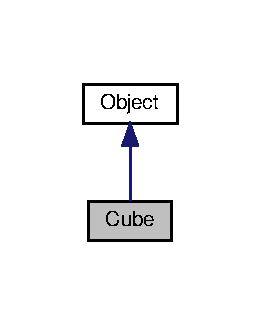
\includegraphics[width=125pt]{classCube__inherit__graph}
\end{center}
\end{figure}


Collaboration diagram for Cube\+:\nopagebreak
\begin{figure}[H]
\begin{center}
\leavevmode
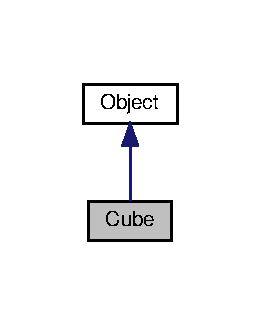
\includegraphics[width=125pt]{classCube__coll__graph}
\end{center}
\end{figure}
\subsection*{Public Member Functions}
\begin{DoxyCompactItemize}
\item 
\hyperlink{classCube_a41a92f10d372f9398b34d9d35d3ef720}{Cube} (std\+::string const \&texture\+Name)
\item 
\hyperlink{classCube_af45ed13232aae0b1271df4f61726a575}{Cube} (std\+::vector$<$ std\+::string $>$ const \&texture\+Name)
\item 
\hyperlink{classCube_a50a1ee10578a47a093c11e5d97ed4a29}{$\sim$\+Cube} () override
\item 
void \hyperlink{classCube_a0dfc84b5634e8c3f0fefd3482085e855}{draw} (sf\+::\+Shader \&shader, glm\+::mat4 \&view, glm\+::mat4 \&projection, glm\+::vec3 const \&position=glm\+::vec3(0.\+0f, 0.\+0f, 0.\+0f), glm\+::vec3 const \&scale=glm\+::vec3(1.\+0f, 1.\+0f, 1.\+0f)) override
\end{DoxyCompactItemize}
\subsection*{Protected Member Functions}
\begin{DoxyCompactItemize}
\item 
void \hyperlink{classCube_a107c29684289fcd3be2b1da6d297fe23}{setup} (std\+::vector$<$ float $>$ const \&vertices) override
\item 
unsigned int \hyperlink{classCube_ad4e00146ffacc5d272aa0c501bee4dca}{init\+Texture} (std\+::string const \&texture\+Name) override
\item 
unsigned int \hyperlink{classCube_a9ffa60b8c97c5419277b0ad2f9a3e92e}{init\+Texture} (std\+::vector$<$ std\+::string $>$ const \&texture\+Name) override
\item 
void \hyperlink{classCube_af4873f0863ce7ad4f37e4af154782a27}{destroy} () override
\end{DoxyCompactItemize}
\subsection*{Additional Inherited Members}


\subsection{Constructor \& Destructor Documentation}
\mbox{\Hypertarget{classCube_a41a92f10d372f9398b34d9d35d3ef720}\label{classCube_a41a92f10d372f9398b34d9d35d3ef720}} 
\index{Cube@{Cube}!Cube@{Cube}}
\index{Cube@{Cube}!Cube@{Cube}}
\subsubsection{\texorpdfstring{Cube()}{Cube()}\hspace{0.1cm}{\footnotesize\ttfamily [1/2]}}
{\footnotesize\ttfamily Cube\+::\+Cube (\begin{DoxyParamCaption}\item[{std\+::string const \&}]{texture\+Name }\end{DoxyParamCaption})}

\mbox{\Hypertarget{classCube_af45ed13232aae0b1271df4f61726a575}\label{classCube_af45ed13232aae0b1271df4f61726a575}} 
\index{Cube@{Cube}!Cube@{Cube}}
\index{Cube@{Cube}!Cube@{Cube}}
\subsubsection{\texorpdfstring{Cube()}{Cube()}\hspace{0.1cm}{\footnotesize\ttfamily [2/2]}}
{\footnotesize\ttfamily Cube\+::\+Cube (\begin{DoxyParamCaption}\item[{std\+::vector$<$ std\+::string $>$ const \&}]{texture\+Name }\end{DoxyParamCaption})}

\mbox{\Hypertarget{classCube_a50a1ee10578a47a093c11e5d97ed4a29}\label{classCube_a50a1ee10578a47a093c11e5d97ed4a29}} 
\index{Cube@{Cube}!````~Cube@{$\sim$\+Cube}}
\index{````~Cube@{$\sim$\+Cube}!Cube@{Cube}}
\subsubsection{\texorpdfstring{$\sim$\+Cube()}{~Cube()}}
{\footnotesize\ttfamily Cube\+::$\sim$\+Cube (\begin{DoxyParamCaption}{ }\end{DoxyParamCaption})\hspace{0.3cm}{\ttfamily [override]}}



\subsection{Member Function Documentation}
\mbox{\Hypertarget{classCube_af4873f0863ce7ad4f37e4af154782a27}\label{classCube_af4873f0863ce7ad4f37e4af154782a27}} 
\index{Cube@{Cube}!destroy@{destroy}}
\index{destroy@{destroy}!Cube@{Cube}}
\subsubsection{\texorpdfstring{destroy()}{destroy()}}
{\footnotesize\ttfamily void Cube\+::destroy (\begin{DoxyParamCaption}{ }\end{DoxyParamCaption})\hspace{0.3cm}{\ttfamily [override]}, {\ttfamily [protected]}, {\ttfamily [virtual]}}



Implements \hyperlink{classObject_a69e91bef2c9f048aa4509329dc44948e}{Object}.

\mbox{\Hypertarget{classCube_a0dfc84b5634e8c3f0fefd3482085e855}\label{classCube_a0dfc84b5634e8c3f0fefd3482085e855}} 
\index{Cube@{Cube}!draw@{draw}}
\index{draw@{draw}!Cube@{Cube}}
\subsubsection{\texorpdfstring{draw()}{draw()}}
{\footnotesize\ttfamily void Cube\+::draw (\begin{DoxyParamCaption}\item[{sf\+::\+Shader \&}]{shader,  }\item[{glm\+::mat4 \&}]{view,  }\item[{glm\+::mat4 \&}]{projection,  }\item[{glm\+::vec3 const \&}]{position = {\ttfamily glm\+:\+:vec3(0.0f,~0.0f,~0.0f)},  }\item[{glm\+::vec3 const \&}]{scale = {\ttfamily glm\+:\+:vec3(1.0f,~1.0f,~1.0f)} }\end{DoxyParamCaption})\hspace{0.3cm}{\ttfamily [override]}, {\ttfamily [virtual]}}



Implements \hyperlink{classObject_ab1ec4e4c64ac1564d9ccad7655cfaf82}{Object}.

\mbox{\Hypertarget{classCube_ad4e00146ffacc5d272aa0c501bee4dca}\label{classCube_ad4e00146ffacc5d272aa0c501bee4dca}} 
\index{Cube@{Cube}!init\+Texture@{init\+Texture}}
\index{init\+Texture@{init\+Texture}!Cube@{Cube}}
\subsubsection{\texorpdfstring{init\+Texture()}{initTexture()}\hspace{0.1cm}{\footnotesize\ttfamily [1/2]}}
{\footnotesize\ttfamily unsigned int Cube\+::init\+Texture (\begin{DoxyParamCaption}\item[{std\+::string const \&}]{texture\+Name }\end{DoxyParamCaption})\hspace{0.3cm}{\ttfamily [override]}, {\ttfamily [protected]}, {\ttfamily [virtual]}}



Implements \hyperlink{classObject_a12b8309292a39b028d5a7b1dfca98cb1}{Object}.

\mbox{\Hypertarget{classCube_a9ffa60b8c97c5419277b0ad2f9a3e92e}\label{classCube_a9ffa60b8c97c5419277b0ad2f9a3e92e}} 
\index{Cube@{Cube}!init\+Texture@{init\+Texture}}
\index{init\+Texture@{init\+Texture}!Cube@{Cube}}
\subsubsection{\texorpdfstring{init\+Texture()}{initTexture()}\hspace{0.1cm}{\footnotesize\ttfamily [2/2]}}
{\footnotesize\ttfamily unsigned int Cube\+::init\+Texture (\begin{DoxyParamCaption}\item[{std\+::vector$<$ std\+::string $>$ const \&}]{texture\+Name }\end{DoxyParamCaption})\hspace{0.3cm}{\ttfamily [override]}, {\ttfamily [protected]}, {\ttfamily [virtual]}}



Implements \hyperlink{classObject_ac18935ff7831cb35dc462b581d2ccf3c}{Object}.

\mbox{\Hypertarget{classCube_a107c29684289fcd3be2b1da6d297fe23}\label{classCube_a107c29684289fcd3be2b1da6d297fe23}} 
\index{Cube@{Cube}!setup@{setup}}
\index{setup@{setup}!Cube@{Cube}}
\subsubsection{\texorpdfstring{setup()}{setup()}}
{\footnotesize\ttfamily void Cube\+::setup (\begin{DoxyParamCaption}\item[{std\+::vector$<$ float $>$ const \&}]{vertices }\end{DoxyParamCaption})\hspace{0.3cm}{\ttfamily [override]}, {\ttfamily [protected]}, {\ttfamily [virtual]}}



Implements \hyperlink{classObject_a262654508b0a6a8cd277911161c71024}{Object}.



The documentation for this class was generated from the following files\+:\begin{DoxyCompactItemize}
\item 
include/\hyperlink{cube_8h}{cube.\+h}\item 
src/\hyperlink{cube_8cpp}{cube.\+cpp}\end{DoxyCompactItemize}

\hypertarget{classHitbox}{}\section{Hitbox Class Reference}
\label{classHitbox}\index{Hitbox@{Hitbox}}


{\ttfamily \#include $<$hitbox.\+h$>$}

\subsection*{Public Member Functions}
\begin{DoxyCompactItemize}
\item 
\hyperlink{classHitbox_a999b0be8486978b3dd7bcd001c7c3c03}{Hitbox} ()
\end{DoxyCompactItemize}
\subsection*{Private Attributes}
\begin{DoxyCompactItemize}
\item 
std\+::vector$<$ glm\+::vec3 $>$ \hyperlink{classHitbox_af424880af1cc55e9096f0758f948cae9}{normal}
\end{DoxyCompactItemize}


\subsection{Constructor \& Destructor Documentation}
\mbox{\Hypertarget{classHitbox_a999b0be8486978b3dd7bcd001c7c3c03}\label{classHitbox_a999b0be8486978b3dd7bcd001c7c3c03}} 
\index{Hitbox@{Hitbox}!Hitbox@{Hitbox}}
\index{Hitbox@{Hitbox}!Hitbox@{Hitbox}}
\subsubsection{\texorpdfstring{Hitbox()}{Hitbox()}}
{\footnotesize\ttfamily Hitbox\+::\+Hitbox (\begin{DoxyParamCaption}{ }\end{DoxyParamCaption})}



\subsection{Member Data Documentation}
\mbox{\Hypertarget{classHitbox_af424880af1cc55e9096f0758f948cae9}\label{classHitbox_af424880af1cc55e9096f0758f948cae9}} 
\index{Hitbox@{Hitbox}!normal@{normal}}
\index{normal@{normal}!Hitbox@{Hitbox}}
\subsubsection{\texorpdfstring{normal}{normal}}
{\footnotesize\ttfamily std\+::vector$<$glm\+::vec3$>$ Hitbox\+::normal\hspace{0.3cm}{\ttfamily [private]}}



The documentation for this class was generated from the following files\+:\begin{DoxyCompactItemize}
\item 
include/\hyperlink{hitbox_8h}{hitbox.\+h}\item 
src/\hyperlink{hitbox_8cpp}{hitbox.\+cpp}\end{DoxyCompactItemize}

\hypertarget{classInstance3D}{}\section{Instance3D Class Reference}
\label{classInstance3D}\index{Instance3D@{Instance3D}}


{\ttfamily \#include $<$instance3\+D.\+h$>$}

\subsection*{Public Member Functions}
\begin{DoxyCompactItemize}
\item 
void \hyperlink{classInstance3D_a6ddedb1613f7dcc885b9b8a722ebd73b}{draw} (glm\+::mat4 \&view, glm\+::mat4 \&projection)
\end{DoxyCompactItemize}
\subsection*{Public Attributes}
\begin{DoxyCompactItemize}
\item 
std\+::unique\+\_\+ptr$<$ \hyperlink{classObject}{Object} $>$ \hyperlink{classInstance3D_af66fce2a9f2854259755505443683056}{object}
\item 
sf\+::\+Shader \hyperlink{classInstance3D_abad4211b399d2be03ffa2ea82ad50d5a}{shader}
\item 
std\+::string \hyperlink{classInstance3D_a93818416ceca4cf47a128fa08c329353}{tag} = \char`\"{}none\char`\"{}
\item 
glm\+::vec3 \hyperlink{classInstance3D_adf6e68d08e5a058e1a1b90e2a0eb435b}{position} = glm\+::vec3(0.\+0f, 0.\+0f, 0.\+0f)
\item 
glm\+::vec3 \hyperlink{classInstance3D_a08b79effaa2e84123c6f768c4a88ae27}{scale} = glm\+::vec3(1.\+0f, 1.\+0f, 1.\+0f)
\end{DoxyCompactItemize}


\subsection{Member Function Documentation}
\mbox{\Hypertarget{classInstance3D_a6ddedb1613f7dcc885b9b8a722ebd73b}\label{classInstance3D_a6ddedb1613f7dcc885b9b8a722ebd73b}} 
\index{Instance3D@{Instance3D}!draw@{draw}}
\index{draw@{draw}!Instance3D@{Instance3D}}
\subsubsection{\texorpdfstring{draw()}{draw()}}
{\footnotesize\ttfamily void Instance3\+D\+::draw (\begin{DoxyParamCaption}\item[{glm\+::mat4 \&}]{view,  }\item[{glm\+::mat4 \&}]{projection }\end{DoxyParamCaption})\hspace{0.3cm}{\ttfamily [inline]}}



\subsection{Member Data Documentation}
\mbox{\Hypertarget{classInstance3D_af66fce2a9f2854259755505443683056}\label{classInstance3D_af66fce2a9f2854259755505443683056}} 
\index{Instance3D@{Instance3D}!object@{object}}
\index{object@{object}!Instance3D@{Instance3D}}
\subsubsection{\texorpdfstring{object}{object}}
{\footnotesize\ttfamily std\+::unique\+\_\+ptr$<$\hyperlink{classObject}{Object}$>$ Instance3\+D\+::object}

\mbox{\Hypertarget{classInstance3D_adf6e68d08e5a058e1a1b90e2a0eb435b}\label{classInstance3D_adf6e68d08e5a058e1a1b90e2a0eb435b}} 
\index{Instance3D@{Instance3D}!position@{position}}
\index{position@{position}!Instance3D@{Instance3D}}
\subsubsection{\texorpdfstring{position}{position}}
{\footnotesize\ttfamily glm\+::vec3 Instance3\+D\+::position = glm\+::vec3(0.\+0f, 0.\+0f, 0.\+0f)}

\mbox{\Hypertarget{classInstance3D_a08b79effaa2e84123c6f768c4a88ae27}\label{classInstance3D_a08b79effaa2e84123c6f768c4a88ae27}} 
\index{Instance3D@{Instance3D}!scale@{scale}}
\index{scale@{scale}!Instance3D@{Instance3D}}
\subsubsection{\texorpdfstring{scale}{scale}}
{\footnotesize\ttfamily glm\+::vec3 Instance3\+D\+::scale = glm\+::vec3(1.\+0f, 1.\+0f, 1.\+0f)}

\mbox{\Hypertarget{classInstance3D_abad4211b399d2be03ffa2ea82ad50d5a}\label{classInstance3D_abad4211b399d2be03ffa2ea82ad50d5a}} 
\index{Instance3D@{Instance3D}!shader@{shader}}
\index{shader@{shader}!Instance3D@{Instance3D}}
\subsubsection{\texorpdfstring{shader}{shader}}
{\footnotesize\ttfamily sf\+::\+Shader Instance3\+D\+::shader}

\mbox{\Hypertarget{classInstance3D_a93818416ceca4cf47a128fa08c329353}\label{classInstance3D_a93818416ceca4cf47a128fa08c329353}} 
\index{Instance3D@{Instance3D}!tag@{tag}}
\index{tag@{tag}!Instance3D@{Instance3D}}
\subsubsection{\texorpdfstring{tag}{tag}}
{\footnotesize\ttfamily std\+::string Instance3\+D\+::tag = \char`\"{}none\char`\"{}}



The documentation for this class was generated from the following file\+:\begin{DoxyCompactItemize}
\item 
include/\hyperlink{instance3D_8h}{instance3\+D.\+h}\end{DoxyCompactItemize}

\hypertarget{classObject}{}\section{Object Class Reference}
\label{classObject}\index{Object@{Object}}


{\ttfamily \#include $<$object.\+h$>$}



Inheritance diagram for Object\+:\nopagebreak
\begin{figure}[H]
\begin{center}
\leavevmode
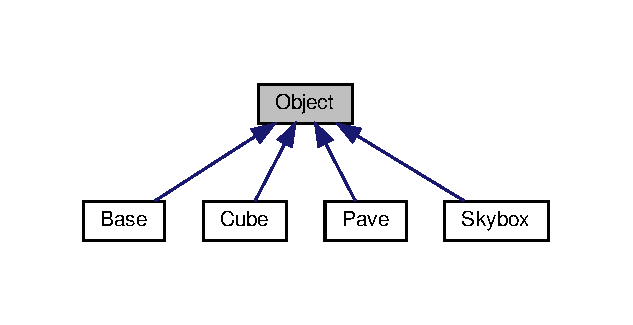
\includegraphics[width=304pt]{classObject__inherit__graph}
\end{center}
\end{figure}
\subsection*{Public Member Functions}
\begin{DoxyCompactItemize}
\item 
\hyperlink{classObject_afe9eeddd7068a37f62d3276a2fb49864}{Object} ()=default
\item 
virtual \hyperlink{classObject_a226f2ae2af766b77d83c09a4d766b725}{$\sim$\+Object} ()=default
\item 
virtual void \hyperlink{classObject_ab1ec4e4c64ac1564d9ccad7655cfaf82}{draw} (sf\+::\+Shader \&shader, glm\+::mat4 \&view, glm\+::mat4 \&projection, glm\+::vec3 const \&position=glm\+::vec3(0.\+0f, 0.\+0f, 0.\+0f), glm\+::vec3 const \&scale=glm\+::vec3(1.\+0f, 1.\+0f, 1.\+0f))=0
\end{DoxyCompactItemize}
\subsection*{Protected Member Functions}
\begin{DoxyCompactItemize}
\item 
virtual void \hyperlink{classObject_a262654508b0a6a8cd277911161c71024}{setup} (std\+::vector$<$ float $>$ const \&vertices)=0
\item 
virtual unsigned int \hyperlink{classObject_a12b8309292a39b028d5a7b1dfca98cb1}{init\+Texture} (std\+::string const \&texture\+Name)=0
\item 
virtual unsigned int \hyperlink{classObject_ac18935ff7831cb35dc462b581d2ccf3c}{init\+Texture} (std\+::vector$<$ std\+::string $>$ const \&texture\+Name)=0
\item 
virtual void \hyperlink{classObject_a69e91bef2c9f048aa4509329dc44948e}{destroy} ()=0
\end{DoxyCompactItemize}
\subsection*{Protected Attributes}
\begin{DoxyCompactItemize}
\item 
unsigned int \hyperlink{classObject_abb132c1ff3bc3c4115f7c48c43f67474}{vertex\+Array\+Object}
\item 
unsigned int \hyperlink{classObject_a2eeb21fc71ed8449cf61d36d99cb0257}{vertex\+Buffer\+Object}
\item 
unsigned int \hyperlink{classObject_a7ed4c3e30bec9ca76a7e820c5d3fdb6d}{texture\+ID}
\end{DoxyCompactItemize}


\subsection{Constructor \& Destructor Documentation}
\mbox{\Hypertarget{classObject_afe9eeddd7068a37f62d3276a2fb49864}\label{classObject_afe9eeddd7068a37f62d3276a2fb49864}} 
\index{Object@{Object}!Object@{Object}}
\index{Object@{Object}!Object@{Object}}
\subsubsection{\texorpdfstring{Object()}{Object()}}
{\footnotesize\ttfamily Object\+::\+Object (\begin{DoxyParamCaption}{ }\end{DoxyParamCaption})\hspace{0.3cm}{\ttfamily [default]}}

\mbox{\Hypertarget{classObject_a226f2ae2af766b77d83c09a4d766b725}\label{classObject_a226f2ae2af766b77d83c09a4d766b725}} 
\index{Object@{Object}!````~Object@{$\sim$\+Object}}
\index{````~Object@{$\sim$\+Object}!Object@{Object}}
\subsubsection{\texorpdfstring{$\sim$\+Object()}{~Object()}}
{\footnotesize\ttfamily virtual Object\+::$\sim$\+Object (\begin{DoxyParamCaption}{ }\end{DoxyParamCaption})\hspace{0.3cm}{\ttfamily [virtual]}, {\ttfamily [default]}}



\subsection{Member Function Documentation}
\mbox{\Hypertarget{classObject_a69e91bef2c9f048aa4509329dc44948e}\label{classObject_a69e91bef2c9f048aa4509329dc44948e}} 
\index{Object@{Object}!destroy@{destroy}}
\index{destroy@{destroy}!Object@{Object}}
\subsubsection{\texorpdfstring{destroy()}{destroy()}}
{\footnotesize\ttfamily virtual void Object\+::destroy (\begin{DoxyParamCaption}{ }\end{DoxyParamCaption})\hspace{0.3cm}{\ttfamily [protected]}, {\ttfamily [pure virtual]}}



Implemented in \hyperlink{classSkybox_a8a93bcf913a1aae88a9a4aa3d20abacc}{Skybox}, \hyperlink{classBase_ac547253cd64e7bc7e4a675eaa4e880b7}{Base}, \hyperlink{classCube_af4873f0863ce7ad4f37e4af154782a27}{Cube}, and \hyperlink{classPave_a1600213efbebd71a3612bb6812ac463b}{Pave}.

\mbox{\Hypertarget{classObject_ab1ec4e4c64ac1564d9ccad7655cfaf82}\label{classObject_ab1ec4e4c64ac1564d9ccad7655cfaf82}} 
\index{Object@{Object}!draw@{draw}}
\index{draw@{draw}!Object@{Object}}
\subsubsection{\texorpdfstring{draw()}{draw()}}
{\footnotesize\ttfamily virtual void Object\+::draw (\begin{DoxyParamCaption}\item[{sf\+::\+Shader \&}]{shader,  }\item[{glm\+::mat4 \&}]{view,  }\item[{glm\+::mat4 \&}]{projection,  }\item[{glm\+::vec3 const \&}]{position = {\ttfamily glm\+:\+:vec3(0.0f,~0.0f,~0.0f)},  }\item[{glm\+::vec3 const \&}]{scale = {\ttfamily glm\+:\+:vec3(1.0f,~1.0f,~1.0f)} }\end{DoxyParamCaption})\hspace{0.3cm}{\ttfamily [pure virtual]}}



Implemented in \hyperlink{classCube_a0dfc84b5634e8c3f0fefd3482085e855}{Cube}, \hyperlink{classSkybox_a6263a420c7ec39e284342988679d3807}{Skybox}, \hyperlink{classBase_ab83ee79d4522f8ad1548d5dd734a3dd5}{Base}, and \hyperlink{classPave_a4dc3714e64f470c05726b7c7200d21e0}{Pave}.

\mbox{\Hypertarget{classObject_a12b8309292a39b028d5a7b1dfca98cb1}\label{classObject_a12b8309292a39b028d5a7b1dfca98cb1}} 
\index{Object@{Object}!init\+Texture@{init\+Texture}}
\index{init\+Texture@{init\+Texture}!Object@{Object}}
\subsubsection{\texorpdfstring{init\+Texture()}{initTexture()}\hspace{0.1cm}{\footnotesize\ttfamily [1/2]}}
{\footnotesize\ttfamily virtual unsigned int Object\+::init\+Texture (\begin{DoxyParamCaption}\item[{std\+::string const \&}]{texture\+Name }\end{DoxyParamCaption})\hspace{0.3cm}{\ttfamily [protected]}, {\ttfamily [pure virtual]}}



Implemented in \hyperlink{classSkybox_a0184f32862c7c46efcce78bde9ee9836}{Skybox}, \hyperlink{classBase_ae1e3b63d1e2d374e1dc49a9160717cfe}{Base}, \hyperlink{classCube_ad4e00146ffacc5d272aa0c501bee4dca}{Cube}, and \hyperlink{classPave_ae3deef5b3908954e34944051f00fea39}{Pave}.

\mbox{\Hypertarget{classObject_ac18935ff7831cb35dc462b581d2ccf3c}\label{classObject_ac18935ff7831cb35dc462b581d2ccf3c}} 
\index{Object@{Object}!init\+Texture@{init\+Texture}}
\index{init\+Texture@{init\+Texture}!Object@{Object}}
\subsubsection{\texorpdfstring{init\+Texture()}{initTexture()}\hspace{0.1cm}{\footnotesize\ttfamily [2/2]}}
{\footnotesize\ttfamily virtual unsigned int Object\+::init\+Texture (\begin{DoxyParamCaption}\item[{std\+::vector$<$ std\+::string $>$ const \&}]{texture\+Name }\end{DoxyParamCaption})\hspace{0.3cm}{\ttfamily [protected]}, {\ttfamily [pure virtual]}}



Implemented in \hyperlink{classSkybox_ae290e8e7374b983c153b581500cd11f3}{Skybox}, \hyperlink{classBase_ae8bcd2edd2c191d58109502792a067ab}{Base}, \hyperlink{classCube_a9ffa60b8c97c5419277b0ad2f9a3e92e}{Cube}, and \hyperlink{classPave_a00f96f2cd410ebc8d95ebc482f79f966}{Pave}.

\mbox{\Hypertarget{classObject_a262654508b0a6a8cd277911161c71024}\label{classObject_a262654508b0a6a8cd277911161c71024}} 
\index{Object@{Object}!setup@{setup}}
\index{setup@{setup}!Object@{Object}}
\subsubsection{\texorpdfstring{setup()}{setup()}}
{\footnotesize\ttfamily virtual void Object\+::setup (\begin{DoxyParamCaption}\item[{std\+::vector$<$ float $>$ const \&}]{vertices }\end{DoxyParamCaption})\hspace{0.3cm}{\ttfamily [protected]}, {\ttfamily [pure virtual]}}



Implemented in \hyperlink{classSkybox_a3f99748c514edd99809a6977f354702f}{Skybox}, \hyperlink{classBase_a57945f86e82faccbd6147f355ed17407}{Base}, \hyperlink{classCube_a107c29684289fcd3be2b1da6d297fe23}{Cube}, and \hyperlink{classPave_a1e3cc420288e7e704891cdfc2cada962}{Pave}.



\subsection{Member Data Documentation}
\mbox{\Hypertarget{classObject_a7ed4c3e30bec9ca76a7e820c5d3fdb6d}\label{classObject_a7ed4c3e30bec9ca76a7e820c5d3fdb6d}} 
\index{Object@{Object}!texture\+ID@{texture\+ID}}
\index{texture\+ID@{texture\+ID}!Object@{Object}}
\subsubsection{\texorpdfstring{texture\+ID}{textureID}}
{\footnotesize\ttfamily unsigned int Object\+::texture\+ID\hspace{0.3cm}{\ttfamily [protected]}}

\mbox{\Hypertarget{classObject_abb132c1ff3bc3c4115f7c48c43f67474}\label{classObject_abb132c1ff3bc3c4115f7c48c43f67474}} 
\index{Object@{Object}!vertex\+Array\+Object@{vertex\+Array\+Object}}
\index{vertex\+Array\+Object@{vertex\+Array\+Object}!Object@{Object}}
\subsubsection{\texorpdfstring{vertex\+Array\+Object}{vertexArrayObject}}
{\footnotesize\ttfamily unsigned int Object\+::vertex\+Array\+Object\hspace{0.3cm}{\ttfamily [protected]}}

\mbox{\Hypertarget{classObject_a2eeb21fc71ed8449cf61d36d99cb0257}\label{classObject_a2eeb21fc71ed8449cf61d36d99cb0257}} 
\index{Object@{Object}!vertex\+Buffer\+Object@{vertex\+Buffer\+Object}}
\index{vertex\+Buffer\+Object@{vertex\+Buffer\+Object}!Object@{Object}}
\subsubsection{\texorpdfstring{vertex\+Buffer\+Object}{vertexBufferObject}}
{\footnotesize\ttfamily unsigned int Object\+::vertex\+Buffer\+Object\hspace{0.3cm}{\ttfamily [protected]}}



The documentation for this class was generated from the following file\+:\begin{DoxyCompactItemize}
\item 
include/\hyperlink{object_8h}{object.\+h}\end{DoxyCompactItemize}

\hypertarget{classPave}{}\section{Pave Class Reference}
\label{classPave}\index{Pave@{Pave}}


{\ttfamily \#include $<$pave.\+h$>$}



Inheritance diagram for Pave\+:\nopagebreak
\begin{figure}[H]
\begin{center}
\leavevmode
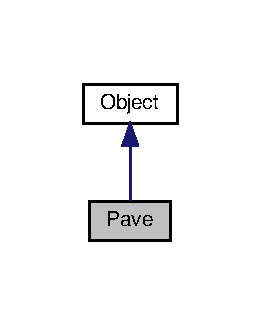
\includegraphics[width=125pt]{classPave__inherit__graph}
\end{center}
\end{figure}


Collaboration diagram for Pave\+:\nopagebreak
\begin{figure}[H]
\begin{center}
\leavevmode
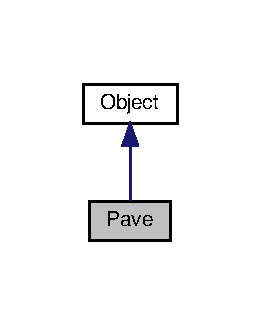
\includegraphics[width=125pt]{classPave__coll__graph}
\end{center}
\end{figure}
\subsection*{Public Member Functions}
\begin{DoxyCompactItemize}
\item 
\hyperlink{classPave_a7537278f91075d65387b8fdb5bed3670}{Pave} (std\+::string const \&texture\+Name)
\item 
\hyperlink{classPave_a78c2b5d920edf472b6f80b914a98b497}{Pave} (std\+::vector$<$ std\+::string $>$ const \&texture\+Name)
\item 
\hyperlink{classPave_ab171241ed7514bb59f563212b9844d6c}{$\sim$\+Pave} () override
\item 
void \hyperlink{classPave_a4dc3714e64f470c05726b7c7200d21e0}{draw} (sf\+::\+Shader \&shader, glm\+::mat4 \&view, glm\+::mat4 \&projection, glm\+::vec3 const \&position=glm\+::vec3(0.\+0f, 0.\+0f, 0.\+0f), glm\+::vec3 const \&scale=glm\+::vec3(1.\+0f, 1.\+0f, 1.\+0f)) override
\end{DoxyCompactItemize}
\subsection*{Protected Member Functions}
\begin{DoxyCompactItemize}
\item 
void \hyperlink{classPave_a1e3cc420288e7e704891cdfc2cada962}{setup} (std\+::vector$<$ float $>$ const \&vertices) override
\item 
unsigned int \hyperlink{classPave_ae3deef5b3908954e34944051f00fea39}{init\+Texture} (std\+::string const \&texture\+Name) override
\item 
unsigned int \hyperlink{classPave_a00f96f2cd410ebc8d95ebc482f79f966}{init\+Texture} (std\+::vector$<$ std\+::string $>$ const \&texture\+Name) override
\item 
void \hyperlink{classPave_a1600213efbebd71a3612bb6812ac463b}{destroy} () override
\end{DoxyCompactItemize}
\subsection*{Additional Inherited Members}


\subsection{Constructor \& Destructor Documentation}
\mbox{\Hypertarget{classPave_a7537278f91075d65387b8fdb5bed3670}\label{classPave_a7537278f91075d65387b8fdb5bed3670}} 
\index{Pave@{Pave}!Pave@{Pave}}
\index{Pave@{Pave}!Pave@{Pave}}
\subsubsection{\texorpdfstring{Pave()}{Pave()}\hspace{0.1cm}{\footnotesize\ttfamily [1/2]}}
{\footnotesize\ttfamily Pave\+::\+Pave (\begin{DoxyParamCaption}\item[{std\+::string const \&}]{texture\+Name }\end{DoxyParamCaption})}

\mbox{\Hypertarget{classPave_a78c2b5d920edf472b6f80b914a98b497}\label{classPave_a78c2b5d920edf472b6f80b914a98b497}} 
\index{Pave@{Pave}!Pave@{Pave}}
\index{Pave@{Pave}!Pave@{Pave}}
\subsubsection{\texorpdfstring{Pave()}{Pave()}\hspace{0.1cm}{\footnotesize\ttfamily [2/2]}}
{\footnotesize\ttfamily Pave\+::\+Pave (\begin{DoxyParamCaption}\item[{std\+::vector$<$ std\+::string $>$ const \&}]{texture\+Name }\end{DoxyParamCaption})}

\mbox{\Hypertarget{classPave_ab171241ed7514bb59f563212b9844d6c}\label{classPave_ab171241ed7514bb59f563212b9844d6c}} 
\index{Pave@{Pave}!````~Pave@{$\sim$\+Pave}}
\index{````~Pave@{$\sim$\+Pave}!Pave@{Pave}}
\subsubsection{\texorpdfstring{$\sim$\+Pave()}{~Pave()}}
{\footnotesize\ttfamily Pave\+::$\sim$\+Pave (\begin{DoxyParamCaption}{ }\end{DoxyParamCaption})\hspace{0.3cm}{\ttfamily [override]}}



\subsection{Member Function Documentation}
\mbox{\Hypertarget{classPave_a1600213efbebd71a3612bb6812ac463b}\label{classPave_a1600213efbebd71a3612bb6812ac463b}} 
\index{Pave@{Pave}!destroy@{destroy}}
\index{destroy@{destroy}!Pave@{Pave}}
\subsubsection{\texorpdfstring{destroy()}{destroy()}}
{\footnotesize\ttfamily void Pave\+::destroy (\begin{DoxyParamCaption}{ }\end{DoxyParamCaption})\hspace{0.3cm}{\ttfamily [override]}, {\ttfamily [protected]}, {\ttfamily [virtual]}}



Implements \hyperlink{classObject_a69e91bef2c9f048aa4509329dc44948e}{Object}.

\mbox{\Hypertarget{classPave_a4dc3714e64f470c05726b7c7200d21e0}\label{classPave_a4dc3714e64f470c05726b7c7200d21e0}} 
\index{Pave@{Pave}!draw@{draw}}
\index{draw@{draw}!Pave@{Pave}}
\subsubsection{\texorpdfstring{draw()}{draw()}}
{\footnotesize\ttfamily void Pave\+::draw (\begin{DoxyParamCaption}\item[{sf\+::\+Shader \&}]{shader,  }\item[{glm\+::mat4 \&}]{view,  }\item[{glm\+::mat4 \&}]{projection,  }\item[{glm\+::vec3 const \&}]{position = {\ttfamily glm\+:\+:vec3(0.0f,~0.0f,~0.0f)},  }\item[{glm\+::vec3 const \&}]{scale = {\ttfamily glm\+:\+:vec3(1.0f,~1.0f,~1.0f)} }\end{DoxyParamCaption})\hspace{0.3cm}{\ttfamily [override]}, {\ttfamily [virtual]}}



Implements \hyperlink{classObject_ab1ec4e4c64ac1564d9ccad7655cfaf82}{Object}.

\mbox{\Hypertarget{classPave_ae3deef5b3908954e34944051f00fea39}\label{classPave_ae3deef5b3908954e34944051f00fea39}} 
\index{Pave@{Pave}!init\+Texture@{init\+Texture}}
\index{init\+Texture@{init\+Texture}!Pave@{Pave}}
\subsubsection{\texorpdfstring{init\+Texture()}{initTexture()}\hspace{0.1cm}{\footnotesize\ttfamily [1/2]}}
{\footnotesize\ttfamily unsigned int Pave\+::init\+Texture (\begin{DoxyParamCaption}\item[{std\+::string const \&}]{texture\+Name }\end{DoxyParamCaption})\hspace{0.3cm}{\ttfamily [override]}, {\ttfamily [protected]}, {\ttfamily [virtual]}}



Implements \hyperlink{classObject_a12b8309292a39b028d5a7b1dfca98cb1}{Object}.

\mbox{\Hypertarget{classPave_a00f96f2cd410ebc8d95ebc482f79f966}\label{classPave_a00f96f2cd410ebc8d95ebc482f79f966}} 
\index{Pave@{Pave}!init\+Texture@{init\+Texture}}
\index{init\+Texture@{init\+Texture}!Pave@{Pave}}
\subsubsection{\texorpdfstring{init\+Texture()}{initTexture()}\hspace{0.1cm}{\footnotesize\ttfamily [2/2]}}
{\footnotesize\ttfamily unsigned int Pave\+::init\+Texture (\begin{DoxyParamCaption}\item[{std\+::vector$<$ std\+::string $>$ const \&}]{texture\+Name }\end{DoxyParamCaption})\hspace{0.3cm}{\ttfamily [override]}, {\ttfamily [protected]}, {\ttfamily [virtual]}}



Implements \hyperlink{classObject_ac18935ff7831cb35dc462b581d2ccf3c}{Object}.

\mbox{\Hypertarget{classPave_a1e3cc420288e7e704891cdfc2cada962}\label{classPave_a1e3cc420288e7e704891cdfc2cada962}} 
\index{Pave@{Pave}!setup@{setup}}
\index{setup@{setup}!Pave@{Pave}}
\subsubsection{\texorpdfstring{setup()}{setup()}}
{\footnotesize\ttfamily void Pave\+::setup (\begin{DoxyParamCaption}\item[{std\+::vector$<$ float $>$ const \&}]{vertices }\end{DoxyParamCaption})\hspace{0.3cm}{\ttfamily [override]}, {\ttfamily [protected]}, {\ttfamily [virtual]}}



Implements \hyperlink{classObject_a262654508b0a6a8cd277911161c71024}{Object}.



The documentation for this class was generated from the following files\+:\begin{DoxyCompactItemize}
\item 
include/\hyperlink{pave_8h}{pave.\+h}\item 
src/\hyperlink{pave_8cpp}{pave.\+cpp}\end{DoxyCompactItemize}

\hypertarget{classScene}{}\section{Scene Class Reference}
\label{classScene}\index{Scene@{Scene}}


{\ttfamily \#include $<$scene.\+h$>$}



Collaboration diagram for Scene\+:\nopagebreak
\begin{figure}[H]
\begin{center}
\leavevmode
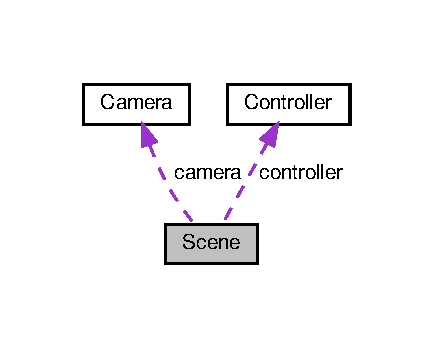
\includegraphics[width=208pt]{classScene__coll__graph}
\end{center}
\end{figure}
\subsection*{Public Member Functions}
\begin{DoxyCompactItemize}
\item 
\hyperlink{classScene_ad10176d75a9cc0da56626f682d083507}{Scene} ()
\item 
void \hyperlink{classScene_abb3b6efc6fdba03cd96436edaf08a967}{init} ()
\item 
void \hyperlink{classScene_a8df1bf2075a891fb2929b58e85d79d34}{loop} ()
\item 
void \hyperlink{classScene_a3ec6a1b861488cd7ef4c31f8ac0ba3f0}{update\+Control} ()
\item 
void \hyperlink{classScene_a25ed345babc6bf277c57085509090f88}{update\+Object} ()
\item 
void \hyperlink{classScene_a1aba87f0c95af84af8aed0d7d3fb40e6}{over} ()
\end{DoxyCompactItemize}
\subsection*{Private Attributes}
\begin{DoxyCompactItemize}
\item 
\hyperlink{classController}{Controller} \hyperlink{classScene_aac14170851aa8186820beae6a2097bc9}{controller}
\item 
\hyperlink{classCamera}{Camera} \hyperlink{classScene_afed13ec4ba2d7ab75b273d507911b498}{camera}
\item 
std\+::unique\+\_\+ptr$<$ sf\+::\+Context\+Settings $>$ \hyperlink{classScene_a23cafa9acb6cc5caa3d3cfa001aea369}{settings}
\item 
std\+::unique\+\_\+ptr$<$ sf\+::\+Window $>$ \hyperlink{classScene_ab8f34017bc48b3c98e16be0ce44adf46}{window}
\item 
std\+::vector$<$ \hyperlink{classInstance3D}{Instance3D} $>$ \hyperlink{classScene_a04300c11c1aaaaae2019e0f9208c9252}{level}
\end{DoxyCompactItemize}


\subsection{Constructor \& Destructor Documentation}
\mbox{\Hypertarget{classScene_ad10176d75a9cc0da56626f682d083507}\label{classScene_ad10176d75a9cc0da56626f682d083507}} 
\index{Scene@{Scene}!Scene@{Scene}}
\index{Scene@{Scene}!Scene@{Scene}}
\subsubsection{\texorpdfstring{Scene()}{Scene()}}
{\footnotesize\ttfamily Scene\+::\+Scene (\begin{DoxyParamCaption}{ }\end{DoxyParamCaption})}



\subsection{Member Function Documentation}
\mbox{\Hypertarget{classScene_abb3b6efc6fdba03cd96436edaf08a967}\label{classScene_abb3b6efc6fdba03cd96436edaf08a967}} 
\index{Scene@{Scene}!init@{init}}
\index{init@{init}!Scene@{Scene}}
\subsubsection{\texorpdfstring{init()}{init()}}
{\footnotesize\ttfamily void Scene\+::init (\begin{DoxyParamCaption}{ }\end{DoxyParamCaption})}

\mbox{\Hypertarget{classScene_a8df1bf2075a891fb2929b58e85d79d34}\label{classScene_a8df1bf2075a891fb2929b58e85d79d34}} 
\index{Scene@{Scene}!loop@{loop}}
\index{loop@{loop}!Scene@{Scene}}
\subsubsection{\texorpdfstring{loop()}{loop()}}
{\footnotesize\ttfamily void Scene\+::loop (\begin{DoxyParamCaption}{ }\end{DoxyParamCaption})}

\mbox{\Hypertarget{classScene_a1aba87f0c95af84af8aed0d7d3fb40e6}\label{classScene_a1aba87f0c95af84af8aed0d7d3fb40e6}} 
\index{Scene@{Scene}!over@{over}}
\index{over@{over}!Scene@{Scene}}
\subsubsection{\texorpdfstring{over()}{over()}}
{\footnotesize\ttfamily void Scene\+::over (\begin{DoxyParamCaption}{ }\end{DoxyParamCaption})}

\mbox{\Hypertarget{classScene_a3ec6a1b861488cd7ef4c31f8ac0ba3f0}\label{classScene_a3ec6a1b861488cd7ef4c31f8ac0ba3f0}} 
\index{Scene@{Scene}!update\+Control@{update\+Control}}
\index{update\+Control@{update\+Control}!Scene@{Scene}}
\subsubsection{\texorpdfstring{update\+Control()}{updateControl()}}
{\footnotesize\ttfamily void Scene\+::update\+Control (\begin{DoxyParamCaption}{ }\end{DoxyParamCaption})}

\mbox{\Hypertarget{classScene_a25ed345babc6bf277c57085509090f88}\label{classScene_a25ed345babc6bf277c57085509090f88}} 
\index{Scene@{Scene}!update\+Object@{update\+Object}}
\index{update\+Object@{update\+Object}!Scene@{Scene}}
\subsubsection{\texorpdfstring{update\+Object()}{updateObject()}}
{\footnotesize\ttfamily void Scene\+::update\+Object (\begin{DoxyParamCaption}{ }\end{DoxyParamCaption})}



\subsection{Member Data Documentation}
\mbox{\Hypertarget{classScene_afed13ec4ba2d7ab75b273d507911b498}\label{classScene_afed13ec4ba2d7ab75b273d507911b498}} 
\index{Scene@{Scene}!camera@{camera}}
\index{camera@{camera}!Scene@{Scene}}
\subsubsection{\texorpdfstring{camera}{camera}}
{\footnotesize\ttfamily \hyperlink{classCamera}{Camera} Scene\+::camera\hspace{0.3cm}{\ttfamily [private]}}

\mbox{\Hypertarget{classScene_aac14170851aa8186820beae6a2097bc9}\label{classScene_aac14170851aa8186820beae6a2097bc9}} 
\index{Scene@{Scene}!controller@{controller}}
\index{controller@{controller}!Scene@{Scene}}
\subsubsection{\texorpdfstring{controller}{controller}}
{\footnotesize\ttfamily \hyperlink{classController}{Controller} Scene\+::controller\hspace{0.3cm}{\ttfamily [private]}}

\mbox{\Hypertarget{classScene_a04300c11c1aaaaae2019e0f9208c9252}\label{classScene_a04300c11c1aaaaae2019e0f9208c9252}} 
\index{Scene@{Scene}!level@{level}}
\index{level@{level}!Scene@{Scene}}
\subsubsection{\texorpdfstring{level}{level}}
{\footnotesize\ttfamily std\+::vector$<$\hyperlink{classInstance3D}{Instance3D}$>$ Scene\+::level\hspace{0.3cm}{\ttfamily [private]}}

\mbox{\Hypertarget{classScene_a23cafa9acb6cc5caa3d3cfa001aea369}\label{classScene_a23cafa9acb6cc5caa3d3cfa001aea369}} 
\index{Scene@{Scene}!settings@{settings}}
\index{settings@{settings}!Scene@{Scene}}
\subsubsection{\texorpdfstring{settings}{settings}}
{\footnotesize\ttfamily std\+::unique\+\_\+ptr$<$sf\+::\+Context\+Settings$>$ Scene\+::settings\hspace{0.3cm}{\ttfamily [private]}}

\mbox{\Hypertarget{classScene_ab8f34017bc48b3c98e16be0ce44adf46}\label{classScene_ab8f34017bc48b3c98e16be0ce44adf46}} 
\index{Scene@{Scene}!window@{window}}
\index{window@{window}!Scene@{Scene}}
\subsubsection{\texorpdfstring{window}{window}}
{\footnotesize\ttfamily std\+::unique\+\_\+ptr$<$sf\+::\+Window$>$ Scene\+::window\hspace{0.3cm}{\ttfamily [private]}}



The documentation for this class was generated from the following files\+:\begin{DoxyCompactItemize}
\item 
include/\hyperlink{scene_8h}{scene.\+h}\item 
src/\hyperlink{scene_8cpp}{scene.\+cpp}\end{DoxyCompactItemize}

\hypertarget{classSkybox}{}\section{Skybox Class Reference}
\label{classSkybox}\index{Skybox@{Skybox}}


{\ttfamily \#include $<$skybox.\+h$>$}



Inheritance diagram for Skybox\+:\nopagebreak
\begin{figure}[H]
\begin{center}
\leavevmode
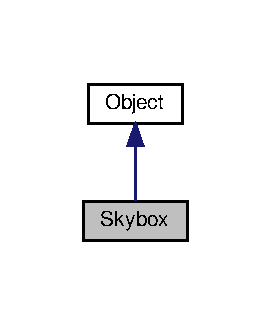
\includegraphics[width=130pt]{classSkybox__inherit__graph}
\end{center}
\end{figure}


Collaboration diagram for Skybox\+:\nopagebreak
\begin{figure}[H]
\begin{center}
\leavevmode
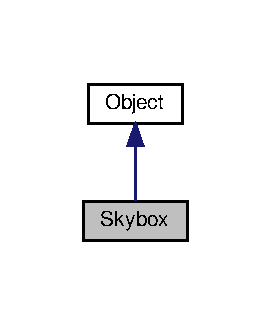
\includegraphics[width=130pt]{classSkybox__coll__graph}
\end{center}
\end{figure}
\subsection*{Public Member Functions}
\begin{DoxyCompactItemize}
\item 
\hyperlink{classSkybox_a9bec390deb9a0f6bd4d8f99237ef6e97}{Skybox} (std\+::vector$<$ std\+::string $>$ \&faces)
\item 
\hyperlink{classSkybox_ae5c2aa5802d7ff5d71192643851a4fd7}{$\sim$\+Skybox} () override
\item 
void \hyperlink{classSkybox_a6263a420c7ec39e284342988679d3807}{draw} (sf\+::\+Shader \&shader, glm\+::mat4 \&view, glm\+::mat4 \&projection, glm\+::vec3 const \&position=glm\+::vec3(0.\+0f, 0.\+0f, 0.\+0f), glm\+::vec3 const \&scale=glm\+::vec3(1.\+0f, 1.\+0f, 1.\+0f)) override
\end{DoxyCompactItemize}
\subsection*{Protected Member Functions}
\begin{DoxyCompactItemize}
\item 
void \hyperlink{classSkybox_a3f99748c514edd99809a6977f354702f}{setup} (std\+::vector$<$ float $>$ const \&vertices) override
\item 
unsigned int \hyperlink{classSkybox_a0184f32862c7c46efcce78bde9ee9836}{init\+Texture} (std\+::string const \&texture\+Name) override
\item 
unsigned int \hyperlink{classSkybox_ae290e8e7374b983c153b581500cd11f3}{init\+Texture} (std\+::vector$<$ std\+::string $>$ const \&faces) override
\item 
void \hyperlink{classSkybox_a8a93bcf913a1aae88a9a4aa3d20abacc}{destroy} () override
\end{DoxyCompactItemize}
\subsection*{Additional Inherited Members}


\subsection{Constructor \& Destructor Documentation}
\mbox{\Hypertarget{classSkybox_a9bec390deb9a0f6bd4d8f99237ef6e97}\label{classSkybox_a9bec390deb9a0f6bd4d8f99237ef6e97}} 
\index{Skybox@{Skybox}!Skybox@{Skybox}}
\index{Skybox@{Skybox}!Skybox@{Skybox}}
\subsubsection{\texorpdfstring{Skybox()}{Skybox()}}
{\footnotesize\ttfamily Skybox\+::\+Skybox (\begin{DoxyParamCaption}\item[{std\+::vector$<$ std\+::string $>$ \&}]{faces }\end{DoxyParamCaption})}

\mbox{\Hypertarget{classSkybox_ae5c2aa5802d7ff5d71192643851a4fd7}\label{classSkybox_ae5c2aa5802d7ff5d71192643851a4fd7}} 
\index{Skybox@{Skybox}!````~Skybox@{$\sim$\+Skybox}}
\index{````~Skybox@{$\sim$\+Skybox}!Skybox@{Skybox}}
\subsubsection{\texorpdfstring{$\sim$\+Skybox()}{~Skybox()}}
{\footnotesize\ttfamily Skybox\+::$\sim$\+Skybox (\begin{DoxyParamCaption}{ }\end{DoxyParamCaption})\hspace{0.3cm}{\ttfamily [override]}}



\subsection{Member Function Documentation}
\mbox{\Hypertarget{classSkybox_a8a93bcf913a1aae88a9a4aa3d20abacc}\label{classSkybox_a8a93bcf913a1aae88a9a4aa3d20abacc}} 
\index{Skybox@{Skybox}!destroy@{destroy}}
\index{destroy@{destroy}!Skybox@{Skybox}}
\subsubsection{\texorpdfstring{destroy()}{destroy()}}
{\footnotesize\ttfamily void Skybox\+::destroy (\begin{DoxyParamCaption}{ }\end{DoxyParamCaption})\hspace{0.3cm}{\ttfamily [override]}, {\ttfamily [protected]}, {\ttfamily [virtual]}}



Implements \hyperlink{classObject_a69e91bef2c9f048aa4509329dc44948e}{Object}.

\mbox{\Hypertarget{classSkybox_a6263a420c7ec39e284342988679d3807}\label{classSkybox_a6263a420c7ec39e284342988679d3807}} 
\index{Skybox@{Skybox}!draw@{draw}}
\index{draw@{draw}!Skybox@{Skybox}}
\subsubsection{\texorpdfstring{draw()}{draw()}}
{\footnotesize\ttfamily void Skybox\+::draw (\begin{DoxyParamCaption}\item[{sf\+::\+Shader \&}]{shader,  }\item[{glm\+::mat4 \&}]{view,  }\item[{glm\+::mat4 \&}]{projection,  }\item[{glm\+::vec3 const \&}]{position = {\ttfamily glm\+:\+:vec3(0.0f,~0.0f,~0.0f)},  }\item[{glm\+::vec3 const \&}]{scale = {\ttfamily glm\+:\+:vec3(1.0f,~1.0f,~1.0f)} }\end{DoxyParamCaption})\hspace{0.3cm}{\ttfamily [override]}, {\ttfamily [virtual]}}



Implements \hyperlink{classObject_ab1ec4e4c64ac1564d9ccad7655cfaf82}{Object}.

\mbox{\Hypertarget{classSkybox_a0184f32862c7c46efcce78bde9ee9836}\label{classSkybox_a0184f32862c7c46efcce78bde9ee9836}} 
\index{Skybox@{Skybox}!init\+Texture@{init\+Texture}}
\index{init\+Texture@{init\+Texture}!Skybox@{Skybox}}
\subsubsection{\texorpdfstring{init\+Texture()}{initTexture()}\hspace{0.1cm}{\footnotesize\ttfamily [1/2]}}
{\footnotesize\ttfamily unsigned int Skybox\+::init\+Texture (\begin{DoxyParamCaption}\item[{std\+::string const \&}]{texture\+Name }\end{DoxyParamCaption})\hspace{0.3cm}{\ttfamily [override]}, {\ttfamily [protected]}, {\ttfamily [virtual]}}



Implements \hyperlink{classObject_a12b8309292a39b028d5a7b1dfca98cb1}{Object}.

\mbox{\Hypertarget{classSkybox_ae290e8e7374b983c153b581500cd11f3}\label{classSkybox_ae290e8e7374b983c153b581500cd11f3}} 
\index{Skybox@{Skybox}!init\+Texture@{init\+Texture}}
\index{init\+Texture@{init\+Texture}!Skybox@{Skybox}}
\subsubsection{\texorpdfstring{init\+Texture()}{initTexture()}\hspace{0.1cm}{\footnotesize\ttfamily [2/2]}}
{\footnotesize\ttfamily unsigned int Skybox\+::init\+Texture (\begin{DoxyParamCaption}\item[{std\+::vector$<$ std\+::string $>$ const \&}]{faces }\end{DoxyParamCaption})\hspace{0.3cm}{\ttfamily [override]}, {\ttfamily [protected]}, {\ttfamily [virtual]}}



Implements \hyperlink{classObject_ac18935ff7831cb35dc462b581d2ccf3c}{Object}.

\mbox{\Hypertarget{classSkybox_a3f99748c514edd99809a6977f354702f}\label{classSkybox_a3f99748c514edd99809a6977f354702f}} 
\index{Skybox@{Skybox}!setup@{setup}}
\index{setup@{setup}!Skybox@{Skybox}}
\subsubsection{\texorpdfstring{setup()}{setup()}}
{\footnotesize\ttfamily void Skybox\+::setup (\begin{DoxyParamCaption}\item[{std\+::vector$<$ float $>$ const \&}]{vertices }\end{DoxyParamCaption})\hspace{0.3cm}{\ttfamily [override]}, {\ttfamily [protected]}, {\ttfamily [virtual]}}



Implements \hyperlink{classObject_a262654508b0a6a8cd277911161c71024}{Object}.



The documentation for this class was generated from the following files\+:\begin{DoxyCompactItemize}
\item 
include/\hyperlink{skybox_8h}{skybox.\+h}\item 
src/\hyperlink{skybox_8cpp}{skybox.\+cpp}\end{DoxyCompactItemize}

\chapter{File Documentation}
\hypertarget{base_8h}{}\section{include/base.h File Reference}
\label{base_8h}\index{include/base.\+h@{include/base.\+h}}
{\ttfamily \#include $<$cube.\+h$>$}\newline
{\ttfamily \#include $<$memory$>$}\newline
{\ttfamily \#include $<$array$>$}\newline
Include dependency graph for base.\+h\+:\nopagebreak
\begin{figure}[H]
\begin{center}
\leavevmode
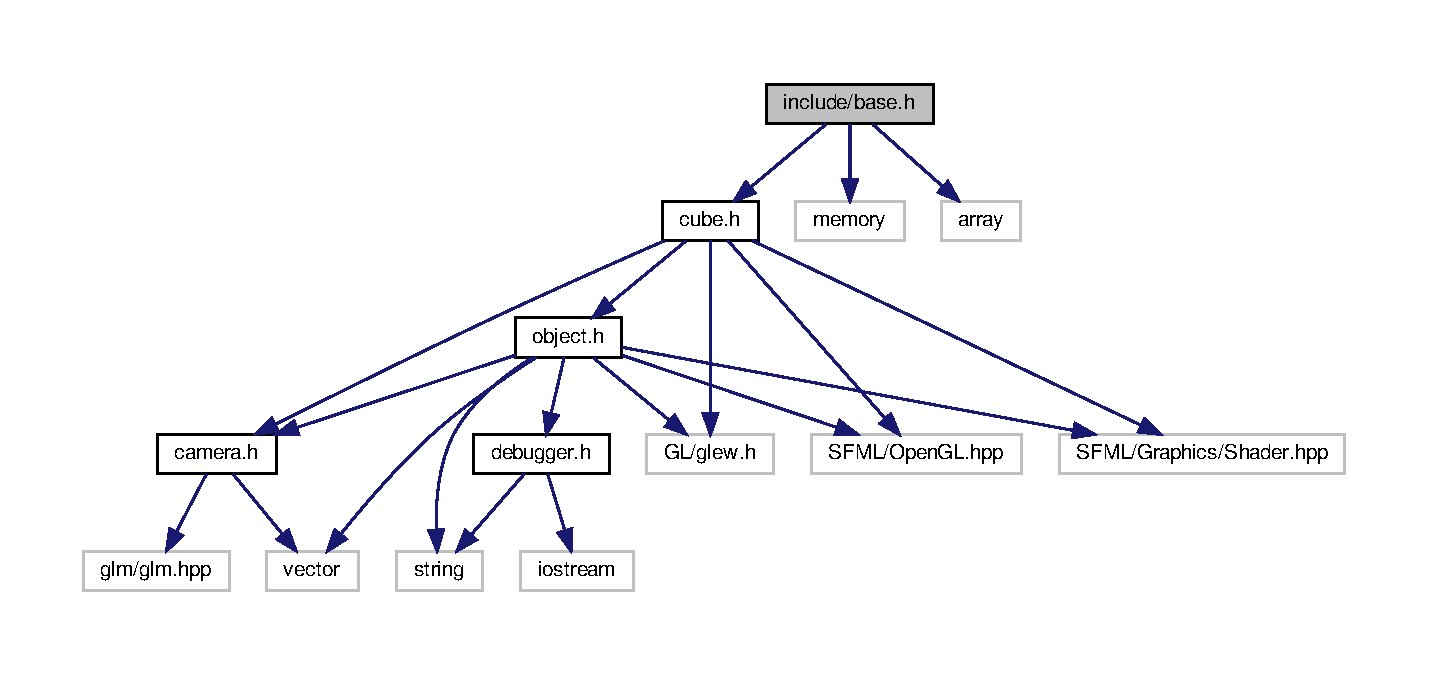
\includegraphics[width=350pt]{base_8h__incl}
\end{center}
\end{figure}
This graph shows which files directly or indirectly include this file\+:\nopagebreak
\begin{figure}[H]
\begin{center}
\leavevmode
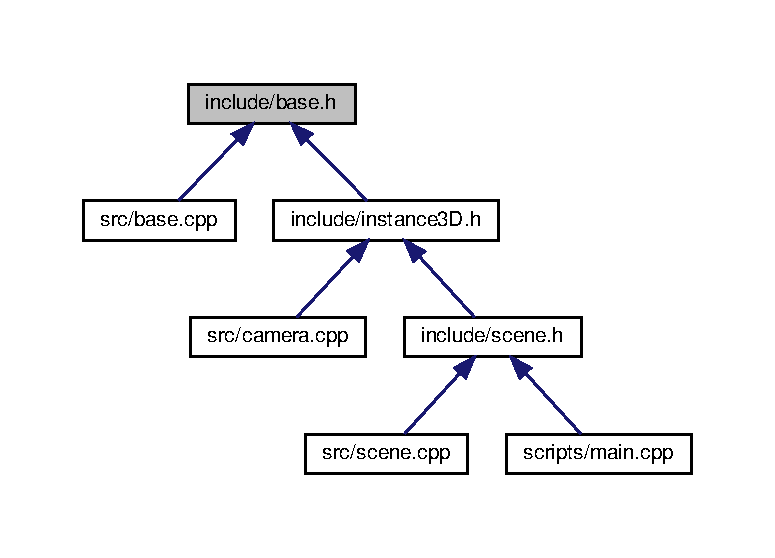
\includegraphics[width=350pt]{base_8h__dep__incl}
\end{center}
\end{figure}
\subsection*{Classes}
\begin{DoxyCompactItemize}
\item 
class \hyperlink{classBase}{Base}
\end{DoxyCompactItemize}

\hypertarget{camera_8h}{}\section{include/camera.h File Reference}
\label{camera_8h}\index{include/camera.\+h@{include/camera.\+h}}
{\ttfamily \#include $<$glm/glm.\+hpp$>$}\newline
{\ttfamily \#include $<$vector$>$}\newline
Include dependency graph for camera.\+h\+:\nopagebreak
\begin{figure}[H]
\begin{center}
\leavevmode
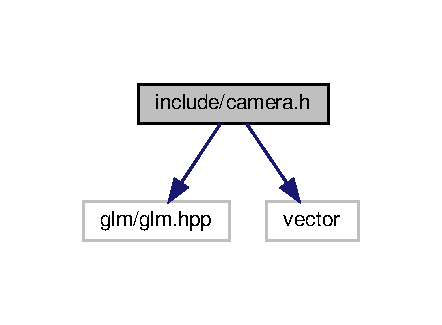
\includegraphics[width=212pt]{camera_8h__incl}
\end{center}
\end{figure}
This graph shows which files directly or indirectly include this file\+:\nopagebreak
\begin{figure}[H]
\begin{center}
\leavevmode
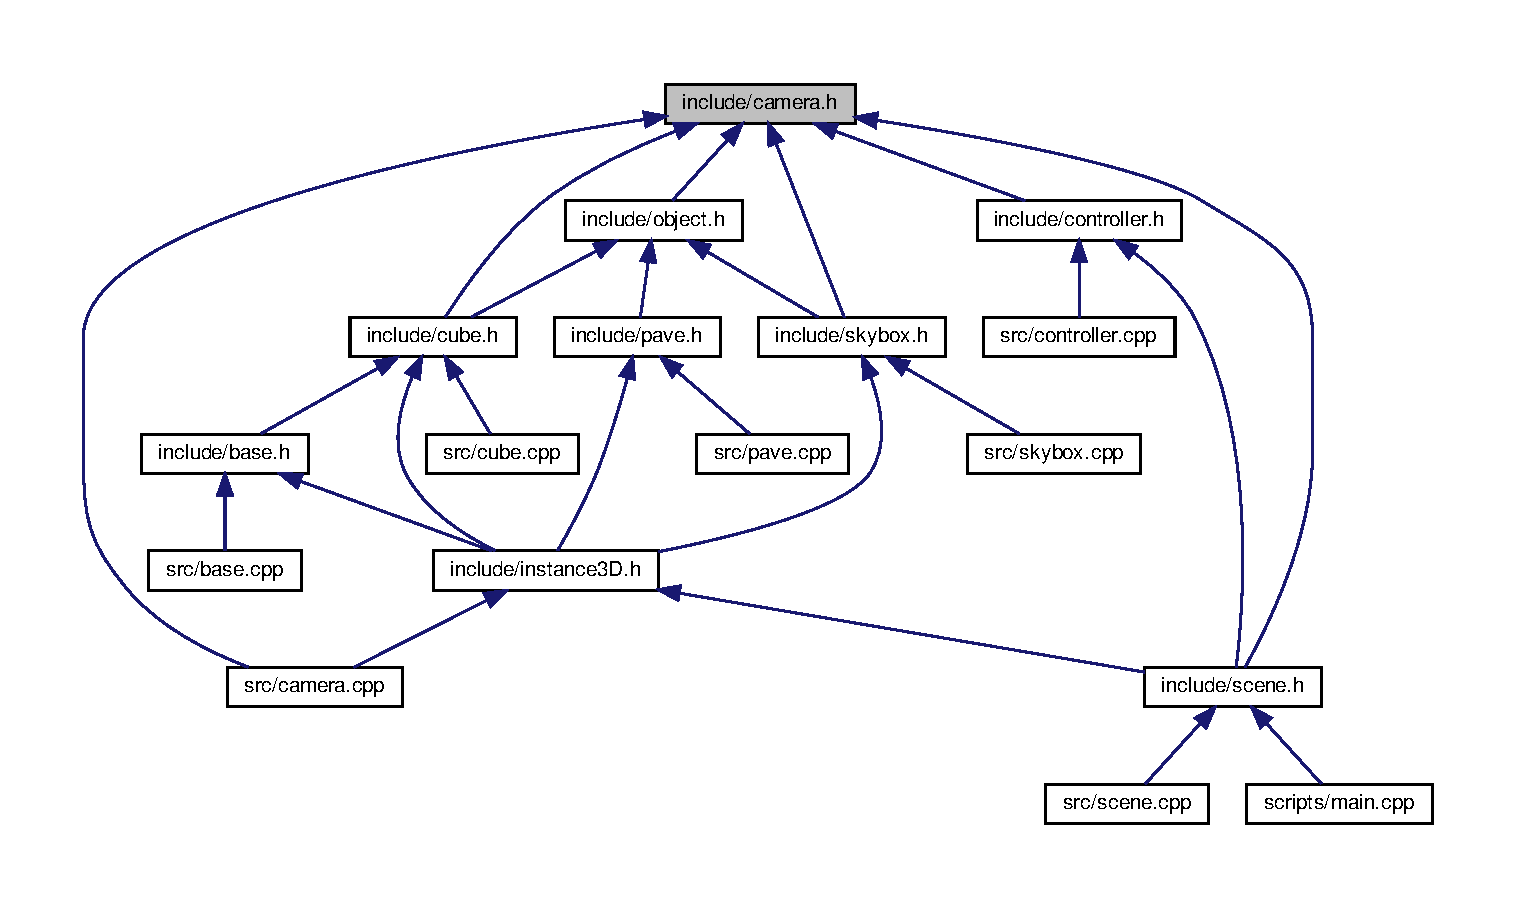
\includegraphics[width=350pt]{camera_8h__dep__incl}
\end{center}
\end{figure}
\subsection*{Classes}
\begin{DoxyCompactItemize}
\item 
class \hyperlink{classCamera}{Camera}
\end{DoxyCompactItemize}
\subsection*{Namespaces}
\begin{DoxyCompactItemize}
\item 
 \hyperlink{namespaceCam}{Cam}
\end{DoxyCompactItemize}
\subsection*{Enumerations}
\begin{DoxyCompactItemize}
\item 
enum \hyperlink{camera_8h_a2fc3593b03b2993ef34f3900f6be985e}{Movement} \{ \hyperlink{camera_8h_a2fc3593b03b2993ef34f3900f6be985eabfec72bb37910c61f36b6c29a1f7ec31}{Movement\+::\+F\+O\+R\+W\+A\+RD}, 
\hyperlink{camera_8h_a2fc3593b03b2993ef34f3900f6be985ea6377b4908ae38f9a57fe9120cf179eb1}{Movement\+::\+B\+A\+C\+K\+W\+A\+RD}, 
\hyperlink{camera_8h_a2fc3593b03b2993ef34f3900f6be985ea684d325a7303f52e64011467ff5c5758}{Movement\+::\+L\+E\+FT}, 
\hyperlink{camera_8h_a2fc3593b03b2993ef34f3900f6be985ea21507b40c80068eda19865706fdc2403}{Movement\+::\+R\+I\+G\+HT}
 \}
\end{DoxyCompactItemize}
\subsection*{Variables}
\begin{DoxyCompactItemize}
\item 
constexpr float \hyperlink{namespaceCam_a19ee86132ca8219870515f550db61f93}{Cam\+::\+Y\+AW} = -\/90.\+0f
\item 
constexpr float \hyperlink{namespaceCam_a5ba61b0ad0aa42c7887436a7f0ac5628}{Cam\+::\+P\+I\+T\+CH} = 0.\+0f
\item 
constexpr float \hyperlink{namespaceCam_a9827a53b18675bb2e3845aadd51e476e}{Cam\+::\+S\+P\+E\+ED} = 20.f
\item 
constexpr float \hyperlink{namespaceCam_a3d86110004c8f438362c6a86532efe9c}{Cam\+::\+S\+E\+N\+S\+I\+T\+I\+V\+I\+TY} = 0.\+1f
\item 
constexpr float \hyperlink{namespaceCam_a44d3e32060d4c50bb27d7110c754cb69}{Cam\+::\+Z\+O\+OM} = 45.\+0f
\item 
constexpr float \hyperlink{namespaceCam_a73d39e25ed690e5a0ea871fb939d9e4d}{Cam\+::\+N\+E\+AR} = 0.\+1f
\item 
constexpr float \hyperlink{namespaceCam_a469e970813928ea23b912618d3401368}{Cam\+::\+F\+AR} = 1000.\+0f
\end{DoxyCompactItemize}


\subsection{Enumeration Type Documentation}
\mbox{\Hypertarget{camera_8h_a2fc3593b03b2993ef34f3900f6be985e}\label{camera_8h_a2fc3593b03b2993ef34f3900f6be985e}} 
\index{camera.\+h@{camera.\+h}!Movement@{Movement}}
\index{Movement@{Movement}!camera.\+h@{camera.\+h}}
\subsubsection{\texorpdfstring{Movement}{Movement}}
{\footnotesize\ttfamily enum \hyperlink{camera_8h_a2fc3593b03b2993ef34f3900f6be985e}{Movement}\hspace{0.3cm}{\ttfamily [strong]}}

\begin{DoxyEnumFields}{Enumerator}
\raisebox{\heightof{T}}[0pt][0pt]{\index{F\+O\+R\+W\+A\+RD@{F\+O\+R\+W\+A\+RD}!camera.\+h@{camera.\+h}}\index{camera.\+h@{camera.\+h}!F\+O\+R\+W\+A\+RD@{F\+O\+R\+W\+A\+RD}}}\mbox{\Hypertarget{camera_8h_a2fc3593b03b2993ef34f3900f6be985eabfec72bb37910c61f36b6c29a1f7ec31}\label{camera_8h_a2fc3593b03b2993ef34f3900f6be985eabfec72bb37910c61f36b6c29a1f7ec31}} 
F\+O\+R\+W\+A\+RD&\\
\hline

\raisebox{\heightof{T}}[0pt][0pt]{\index{B\+A\+C\+K\+W\+A\+RD@{B\+A\+C\+K\+W\+A\+RD}!camera.\+h@{camera.\+h}}\index{camera.\+h@{camera.\+h}!B\+A\+C\+K\+W\+A\+RD@{B\+A\+C\+K\+W\+A\+RD}}}\mbox{\Hypertarget{camera_8h_a2fc3593b03b2993ef34f3900f6be985ea6377b4908ae38f9a57fe9120cf179eb1}\label{camera_8h_a2fc3593b03b2993ef34f3900f6be985ea6377b4908ae38f9a57fe9120cf179eb1}} 
B\+A\+C\+K\+W\+A\+RD&\\
\hline

\raisebox{\heightof{T}}[0pt][0pt]{\index{L\+E\+FT@{L\+E\+FT}!camera.\+h@{camera.\+h}}\index{camera.\+h@{camera.\+h}!L\+E\+FT@{L\+E\+FT}}}\mbox{\Hypertarget{camera_8h_a2fc3593b03b2993ef34f3900f6be985ea684d325a7303f52e64011467ff5c5758}\label{camera_8h_a2fc3593b03b2993ef34f3900f6be985ea684d325a7303f52e64011467ff5c5758}} 
L\+E\+FT&\\
\hline

\raisebox{\heightof{T}}[0pt][0pt]{\index{R\+I\+G\+HT@{R\+I\+G\+HT}!camera.\+h@{camera.\+h}}\index{camera.\+h@{camera.\+h}!R\+I\+G\+HT@{R\+I\+G\+HT}}}\mbox{\Hypertarget{camera_8h_a2fc3593b03b2993ef34f3900f6be985ea21507b40c80068eda19865706fdc2403}\label{camera_8h_a2fc3593b03b2993ef34f3900f6be985ea21507b40c80068eda19865706fdc2403}} 
R\+I\+G\+HT&\\
\hline

\end{DoxyEnumFields}

\hypertarget{controller_8h}{}\section{include/controller.h File Reference}
\label{controller_8h}\index{include/controller.\+h@{include/controller.\+h}}
{\ttfamily \#include $<$camera.\+h$>$}\newline
{\ttfamily \#include $<$S\+F\+M\+L/\+Window/\+Mouse.\+hpp$>$}\newline
{\ttfamily \#include $<$S\+F\+M\+L/\+Window/\+Keyboard.\+hpp$>$}\newline
{\ttfamily \#include $<$S\+F\+M\+L/\+Window/\+Event.\+hpp$>$}\newline
Include dependency graph for controller.\+h\+:\nopagebreak
\begin{figure}[H]
\begin{center}
\leavevmode
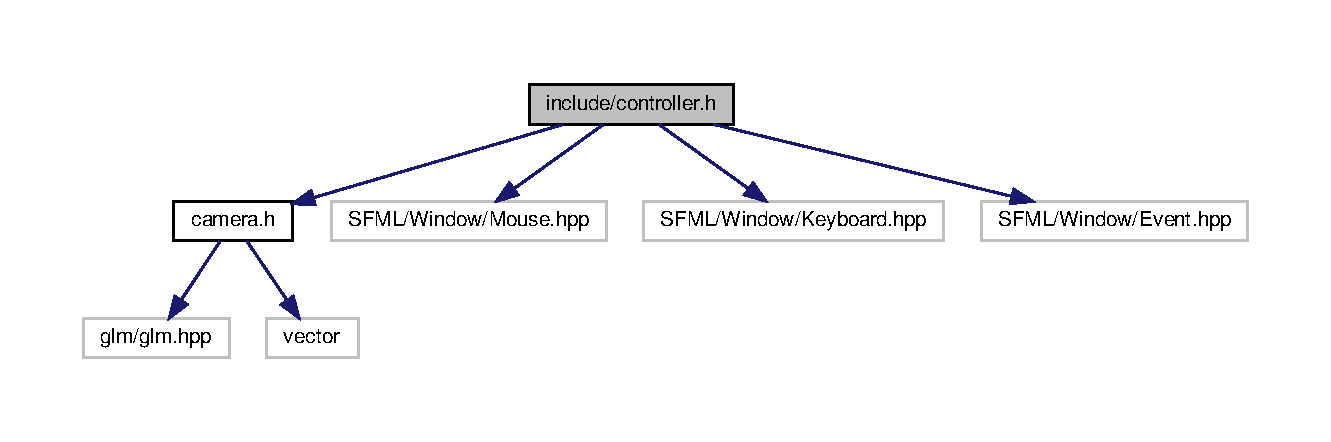
\includegraphics[width=350pt]{controller_8h__incl}
\end{center}
\end{figure}
This graph shows which files directly or indirectly include this file\+:\nopagebreak
\begin{figure}[H]
\begin{center}
\leavevmode
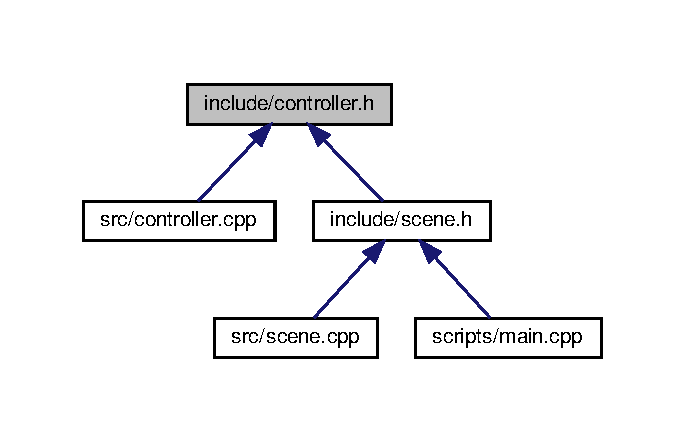
\includegraphics[width=329pt]{controller_8h__dep__incl}
\end{center}
\end{figure}
\subsection*{Classes}
\begin{DoxyCompactItemize}
\item 
class \hyperlink{classController}{Controller}
\end{DoxyCompactItemize}
\subsection*{Namespaces}
\begin{DoxyCompactItemize}
\item 
 \hyperlink{namespaceControl}{Control}
\end{DoxyCompactItemize}
\subsection*{Variables}
\begin{DoxyCompactItemize}
\item 
constexpr float \hyperlink{namespaceControl_a56babc87b3c7df1aba525ccd3e80abf7}{Control\+::\+S\+P\+E\+ED} = 0.\+01f
\item 
constexpr float \hyperlink{namespaceControl_a04a945fadad95f496ca4e1f3d870881a}{Control\+::\+J\+U\+MP} = 0.\+01f
\end{DoxyCompactItemize}

\hypertarget{cube_8h}{}\section{include/cube.h File Reference}
\label{cube_8h}\index{include/cube.\+h@{include/cube.\+h}}
{\ttfamily \#include $<$camera.\+h$>$}\newline
{\ttfamily \#include $<$object.\+h$>$}\newline
{\ttfamily \#include $<$G\+L/glew.\+h$>$}\newline
{\ttfamily \#include $<$S\+F\+M\+L/\+Open\+G\+L.\+hpp$>$}\newline
{\ttfamily \#include $<$S\+F\+M\+L/\+Graphics/\+Shader.\+hpp$>$}\newline
Include dependency graph for cube.\+h\+:\nopagebreak
\begin{figure}[H]
\begin{center}
\leavevmode
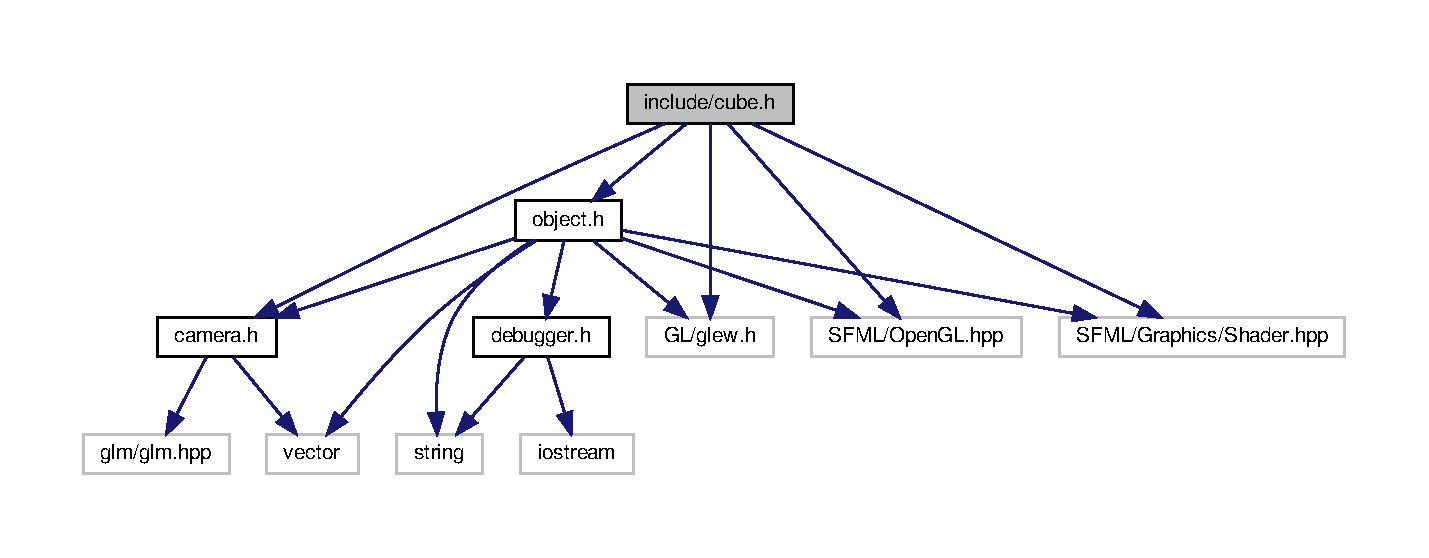
\includegraphics[width=350pt]{cube_8h__incl}
\end{center}
\end{figure}
This graph shows which files directly or indirectly include this file\+:\nopagebreak
\begin{figure}[H]
\begin{center}
\leavevmode
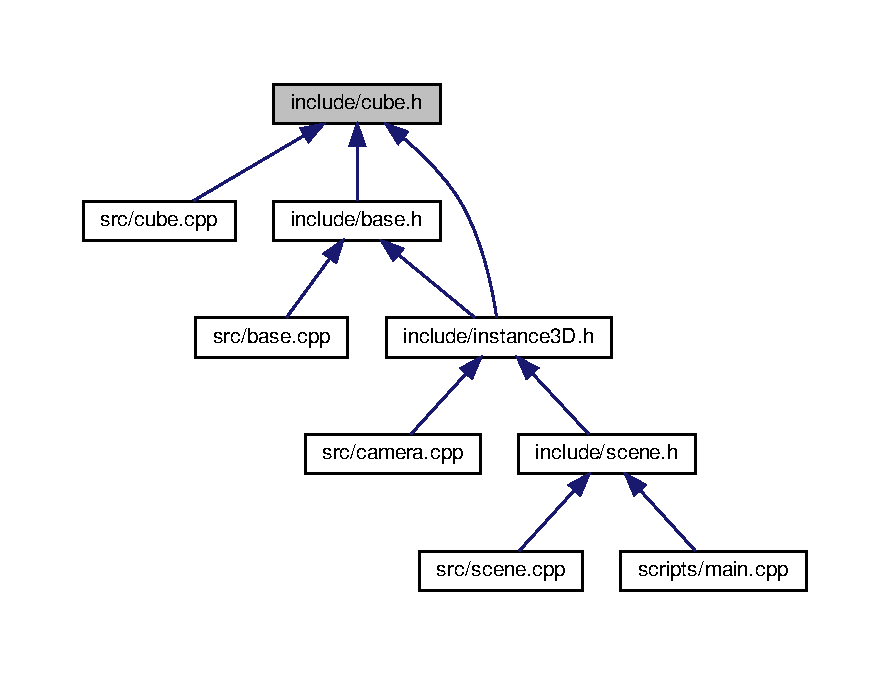
\includegraphics[width=350pt]{cube_8h__dep__incl}
\end{center}
\end{figure}
\subsection*{Classes}
\begin{DoxyCompactItemize}
\item 
class \hyperlink{classCube}{Cube}
\end{DoxyCompactItemize}

\hypertarget{debugger_8h}{}\section{include/debugger.h File Reference}
\label{debugger_8h}\index{include/debugger.\+h@{include/debugger.\+h}}
{\ttfamily \#include $<$string$>$}\newline
{\ttfamily \#include $<$iostream$>$}\newline
Include dependency graph for debugger.\+h\+:\nopagebreak
\begin{figure}[H]
\begin{center}
\leavevmode
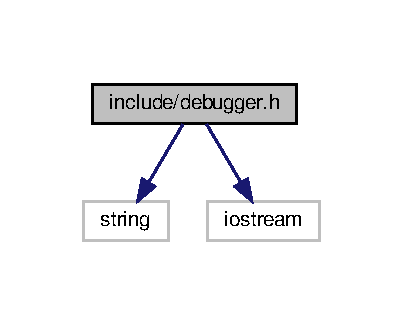
\includegraphics[width=194pt]{debugger_8h__incl}
\end{center}
\end{figure}
This graph shows which files directly or indirectly include this file\+:\nopagebreak
\begin{figure}[H]
\begin{center}
\leavevmode
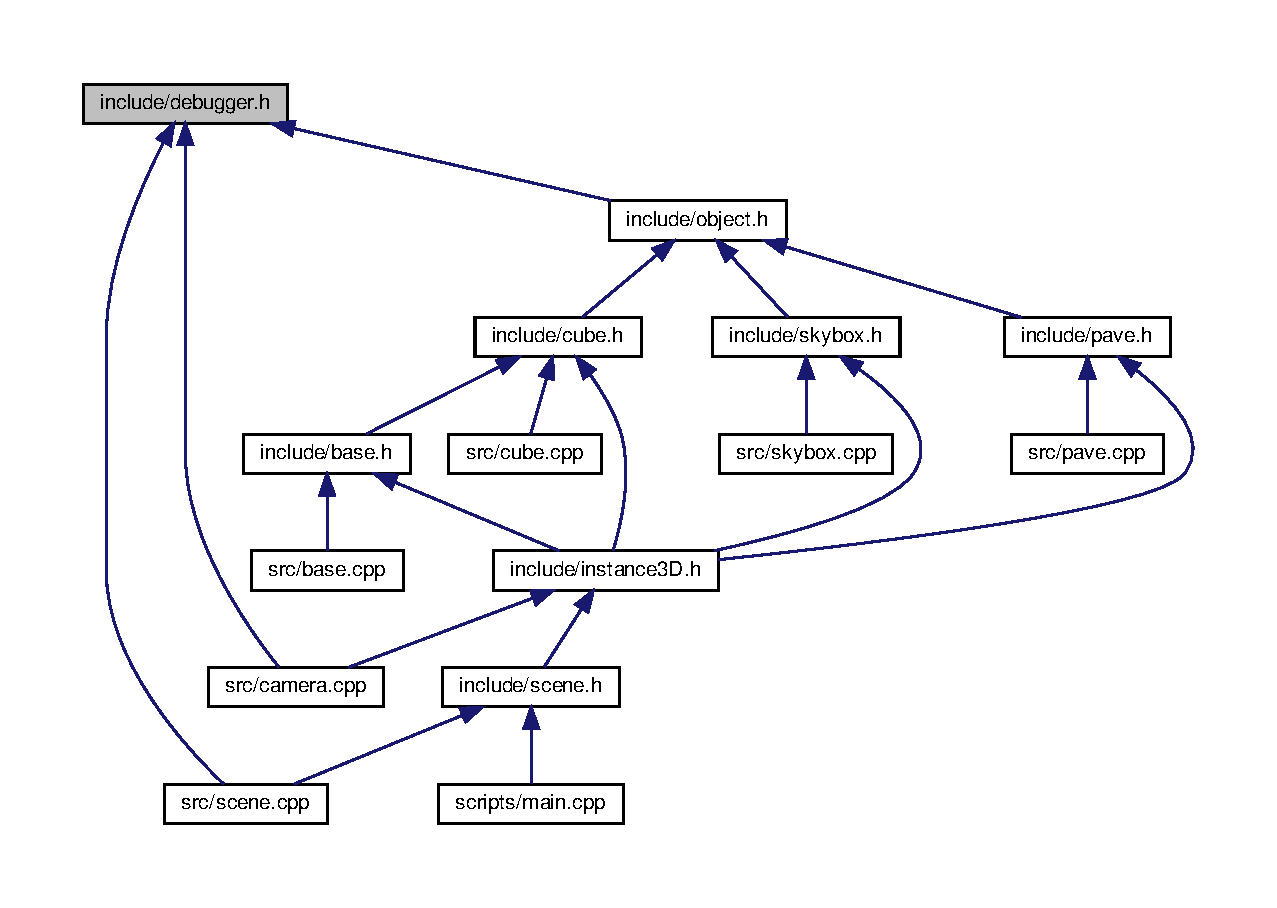
\includegraphics[width=350pt]{debugger_8h__dep__incl}
\end{center}
\end{figure}
\subsection*{Functions}
\begin{DoxyCompactItemize}
\item 
void \hyperlink{debugger_8h_ae919bb5a3a8a684e974c369b3a70ca74}{Log} (std\+::string const \&message)
\item 
{\footnotesize template$<$typename T $>$ }\\void \hyperlink{debugger_8h_a7d00b346db2c0d9168612da4a068d681}{Log} (T const \&object, std\+::string const \&message=\char`\"{}log \+: \char`\"{})
\end{DoxyCompactItemize}


\subsection{Function Documentation}
\mbox{\Hypertarget{debugger_8h_ae919bb5a3a8a684e974c369b3a70ca74}\label{debugger_8h_ae919bb5a3a8a684e974c369b3a70ca74}} 
\index{debugger.\+h@{debugger.\+h}!Log@{Log}}
\index{Log@{Log}!debugger.\+h@{debugger.\+h}}
\subsubsection{\texorpdfstring{Log()}{Log()}\hspace{0.1cm}{\footnotesize\ttfamily [1/2]}}
{\footnotesize\ttfamily void Log (\begin{DoxyParamCaption}\item[{std\+::string const \&}]{message }\end{DoxyParamCaption})\hspace{0.3cm}{\ttfamily [inline]}}

\mbox{\Hypertarget{debugger_8h_a7d00b346db2c0d9168612da4a068d681}\label{debugger_8h_a7d00b346db2c0d9168612da4a068d681}} 
\index{debugger.\+h@{debugger.\+h}!Log@{Log}}
\index{Log@{Log}!debugger.\+h@{debugger.\+h}}
\subsubsection{\texorpdfstring{Log()}{Log()}\hspace{0.1cm}{\footnotesize\ttfamily [2/2]}}
{\footnotesize\ttfamily template$<$typename T $>$ \\
void Log (\begin{DoxyParamCaption}\item[{T const \&}]{object,  }\item[{std\+::string const \&}]{message = {\ttfamily \char`\"{}log~\+:~\char`\"{}} }\end{DoxyParamCaption})\hspace{0.3cm}{\ttfamily [inline]}}


\hypertarget{hitbox_8h}{}\section{include/hitbox.h File Reference}
\label{hitbox_8h}\index{include/hitbox.\+h@{include/hitbox.\+h}}
{\ttfamily \#include $<$glm/glm.\+hpp$>$}\newline
{\ttfamily \#include $<$vector$>$}\newline
Include dependency graph for hitbox.\+h\+:\nopagebreak
\begin{figure}[H]
\begin{center}
\leavevmode
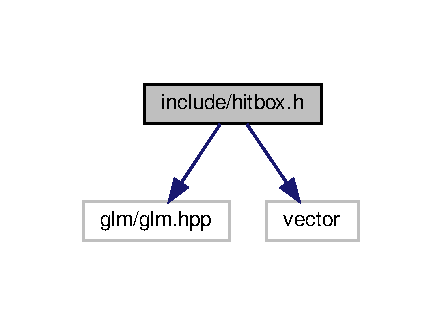
\includegraphics[width=212pt]{hitbox_8h__incl}
\end{center}
\end{figure}
This graph shows which files directly or indirectly include this file\+:\nopagebreak
\begin{figure}[H]
\begin{center}
\leavevmode
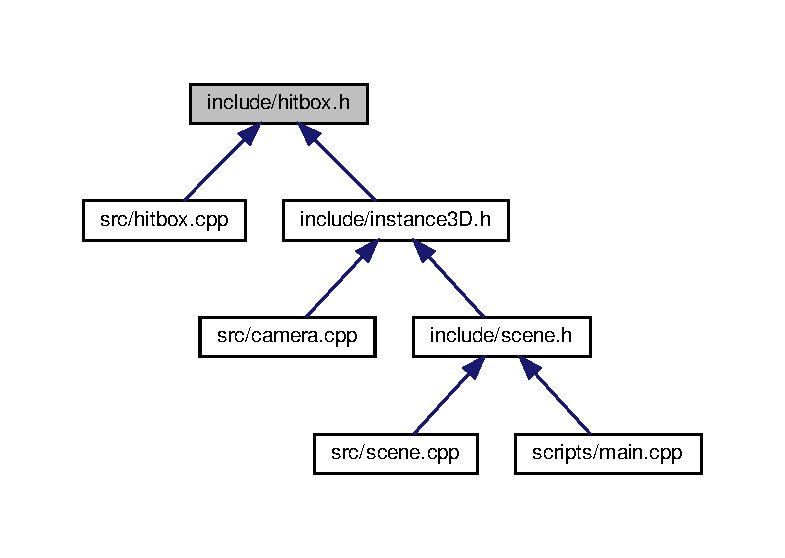
\includegraphics[width=350pt]{hitbox_8h__dep__incl}
\end{center}
\end{figure}
\subsection*{Classes}
\begin{DoxyCompactItemize}
\item 
class \hyperlink{classHitbox}{Hitbox}
\end{DoxyCompactItemize}

\hypertarget{instance3D_8h}{}\section{include/instance3D.h File Reference}
\label{instance3D_8h}\index{include/instance3\+D.\+h@{include/instance3\+D.\+h}}
{\ttfamily \#include $<$skybox.\+h$>$}\newline
{\ttfamily \#include $<$cube.\+h$>$}\newline
{\ttfamily \#include $<$base.\+h$>$}\newline
{\ttfamily \#include $<$pave.\+h$>$}\newline
{\ttfamily \#include $<$hitbox.\+h$>$}\newline
Include dependency graph for instance3\+D.\+h\+:\nopagebreak
\begin{figure}[H]
\begin{center}
\leavevmode
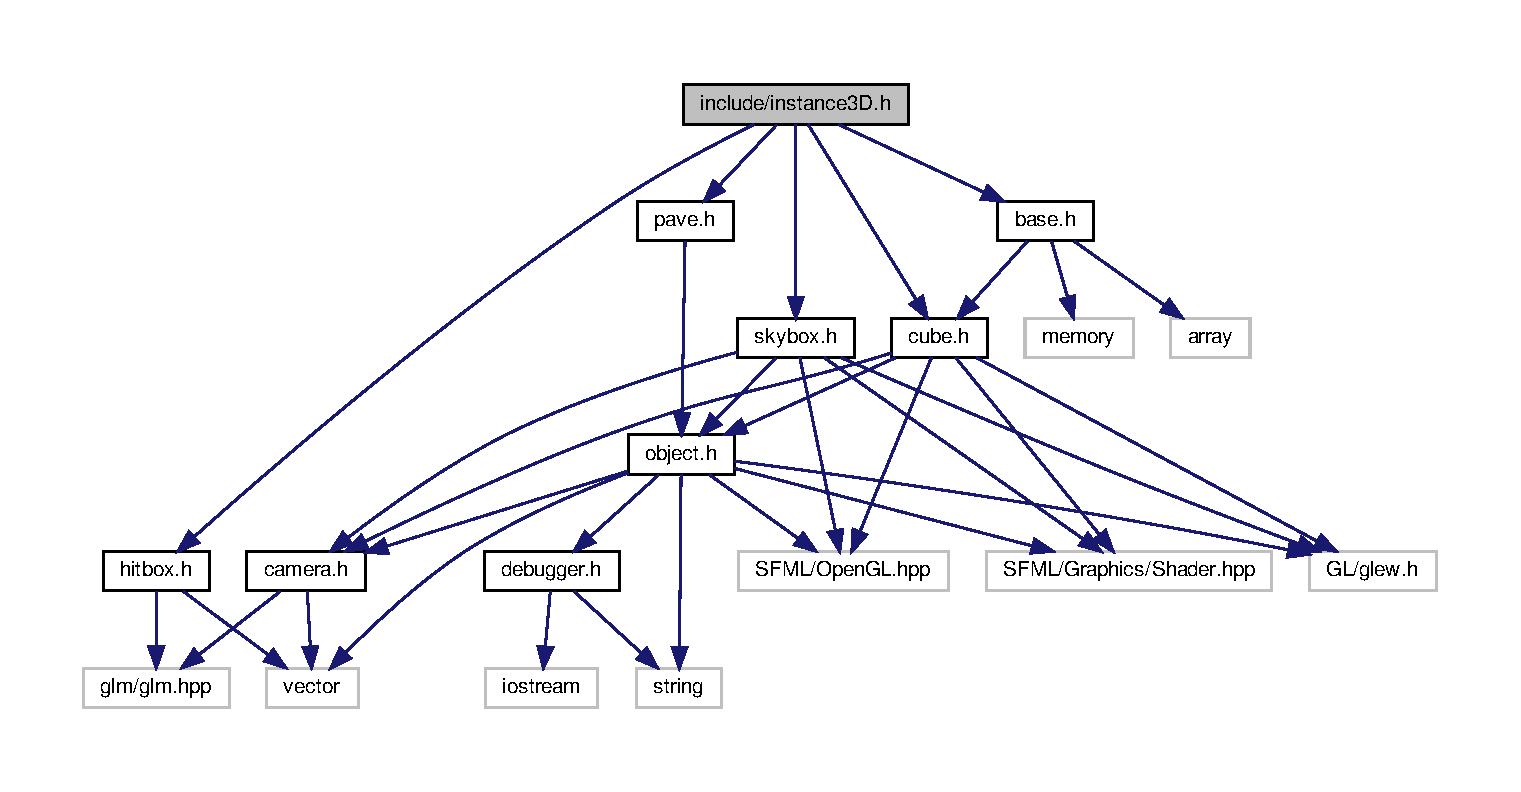
\includegraphics[width=350pt]{instance3D_8h__incl}
\end{center}
\end{figure}
This graph shows which files directly or indirectly include this file\+:\nopagebreak
\begin{figure}[H]
\begin{center}
\leavevmode
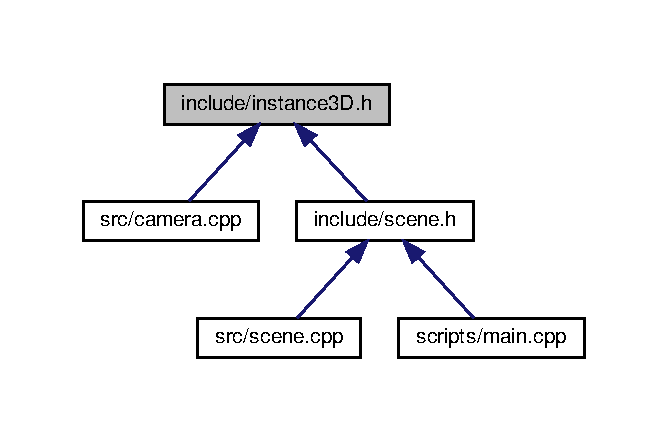
\includegraphics[width=321pt]{instance3D_8h__dep__incl}
\end{center}
\end{figure}
\subsection*{Classes}
\begin{DoxyCompactItemize}
\item 
class \hyperlink{classInstance3D}{Instance3D}
\end{DoxyCompactItemize}

\hypertarget{object_8h}{}\section{include/object.h File Reference}
\label{object_8h}\index{include/object.\+h@{include/object.\+h}}
{\ttfamily \#include $<$camera.\+h$>$}\newline
{\ttfamily \#include $<$debugger.\+h$>$}\newline
{\ttfamily \#include $<$G\+L/glew.\+h$>$}\newline
{\ttfamily \#include $<$S\+F\+M\+L/\+Open\+G\+L.\+hpp$>$}\newline
{\ttfamily \#include $<$S\+F\+M\+L/\+Graphics/\+Shader.\+hpp$>$}\newline
{\ttfamily \#include $<$vector$>$}\newline
{\ttfamily \#include $<$string$>$}\newline
Include dependency graph for object.\+h\+:\nopagebreak
\begin{figure}[H]
\begin{center}
\leavevmode
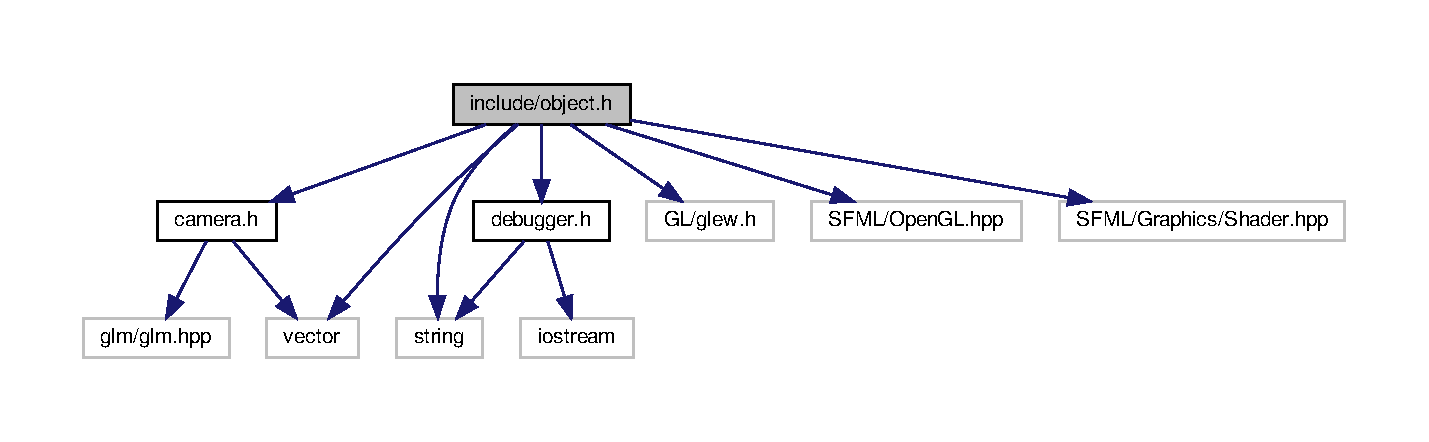
\includegraphics[width=350pt]{object_8h__incl}
\end{center}
\end{figure}
This graph shows which files directly or indirectly include this file\+:\nopagebreak
\begin{figure}[H]
\begin{center}
\leavevmode
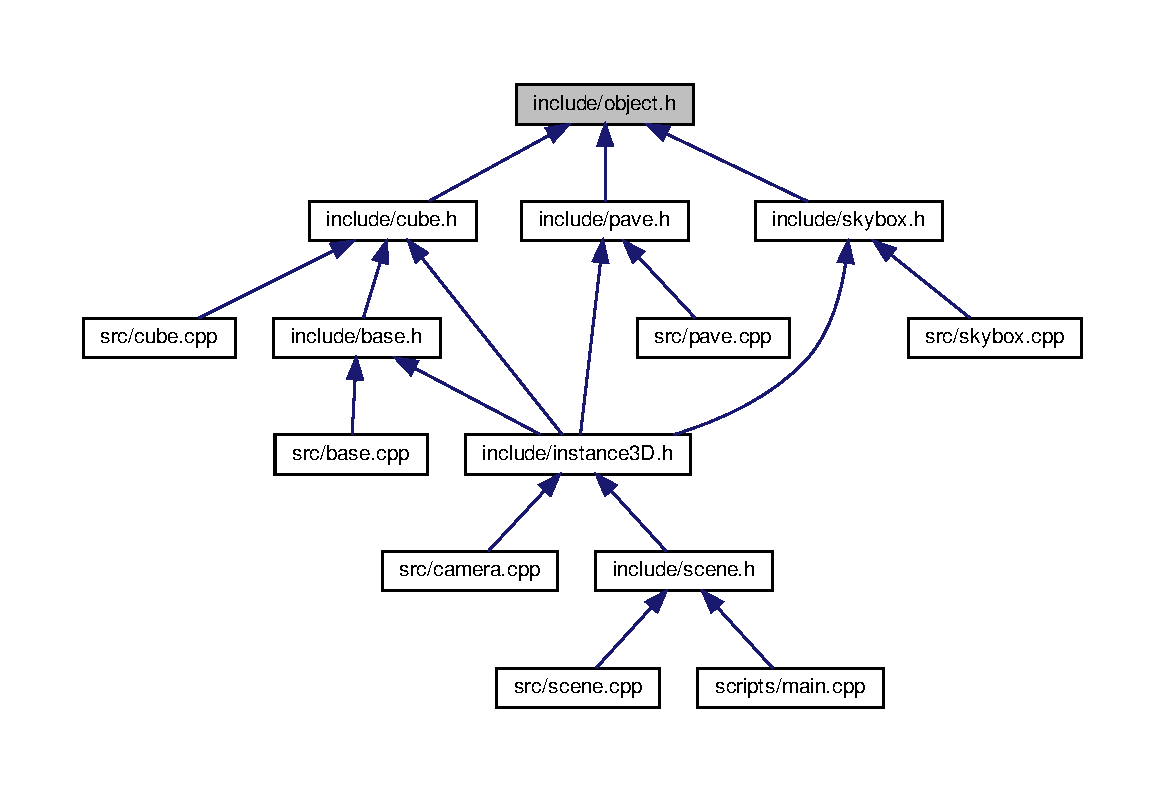
\includegraphics[width=350pt]{object_8h__dep__incl}
\end{center}
\end{figure}
\subsection*{Classes}
\begin{DoxyCompactItemize}
\item 
class \hyperlink{classObject}{Object}
\end{DoxyCompactItemize}

\hypertarget{pave_8h}{}\section{include/pave.h File Reference}
\label{pave_8h}\index{include/pave.\+h@{include/pave.\+h}}
{\ttfamily \#include $<$object.\+h$>$}\newline
Include dependency graph for pave.\+h\+:\nopagebreak
\begin{figure}[H]
\begin{center}
\leavevmode
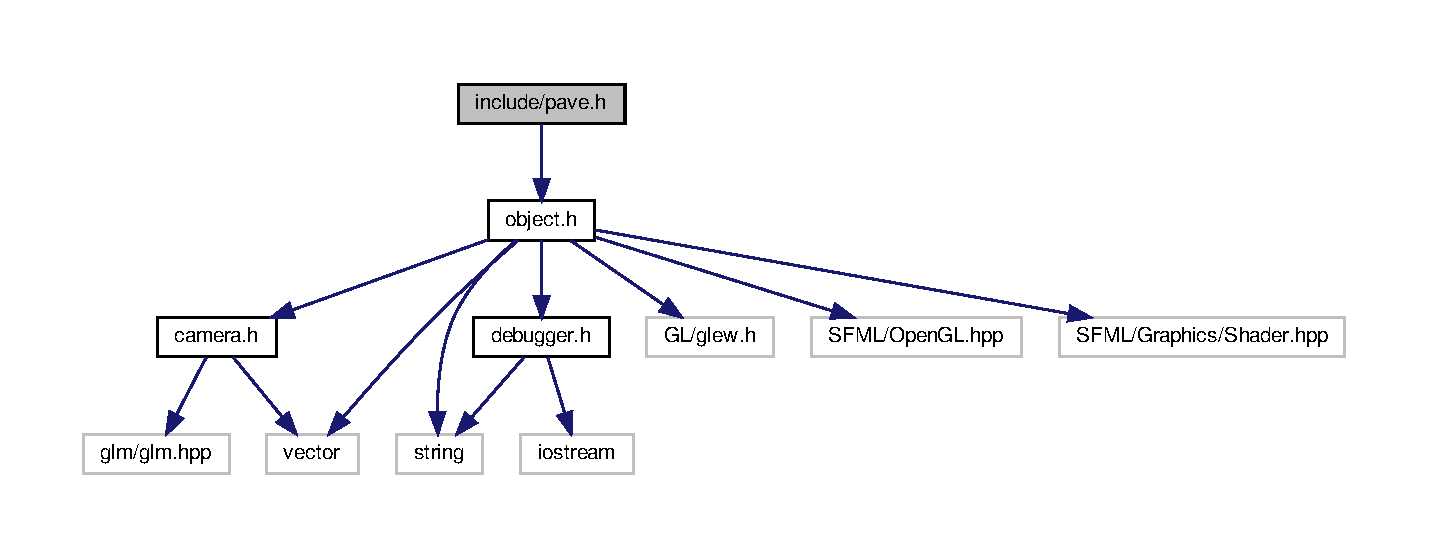
\includegraphics[width=350pt]{pave_8h__incl}
\end{center}
\end{figure}
This graph shows which files directly or indirectly include this file\+:\nopagebreak
\begin{figure}[H]
\begin{center}
\leavevmode
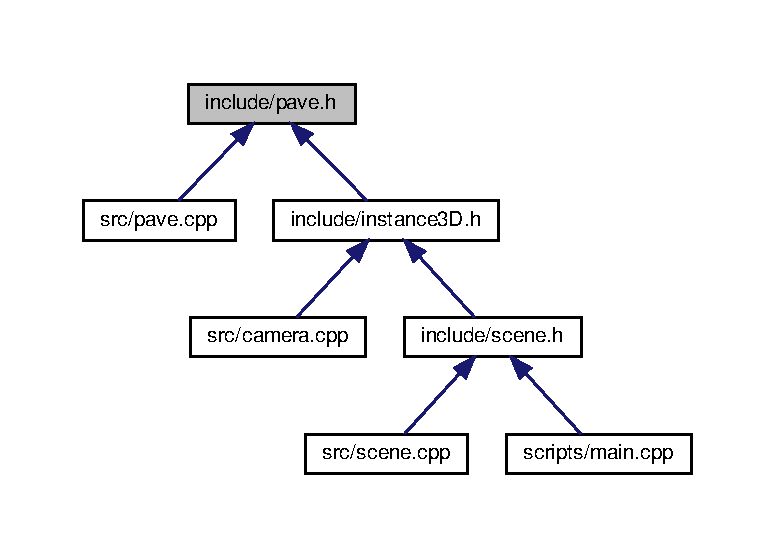
\includegraphics[width=350pt]{pave_8h__dep__incl}
\end{center}
\end{figure}
\subsection*{Classes}
\begin{DoxyCompactItemize}
\item 
class \hyperlink{classPave}{Pave}
\end{DoxyCompactItemize}

\hypertarget{scene_8h}{}\section{include/scene.h File Reference}
\label{scene_8h}\index{include/scene.\+h@{include/scene.\+h}}
{\ttfamily \#include $<$camera.\+h$>$}\newline
{\ttfamily \#include $<$controller.\+h$>$}\newline
{\ttfamily \#include $<$instance3\+D.\+h$>$}\newline
{\ttfamily \#include $<$S\+F\+M\+L/\+Window/\+Context\+Settings.\+hpp$>$}\newline
{\ttfamily \#include $<$S\+F\+M\+L/\+Graphics/\+Render\+Window.\+hpp$>$}\newline
{\ttfamily \#include $<$memory$>$}\newline
Include dependency graph for scene.\+h\+:\nopagebreak
\begin{figure}[H]
\begin{center}
\leavevmode
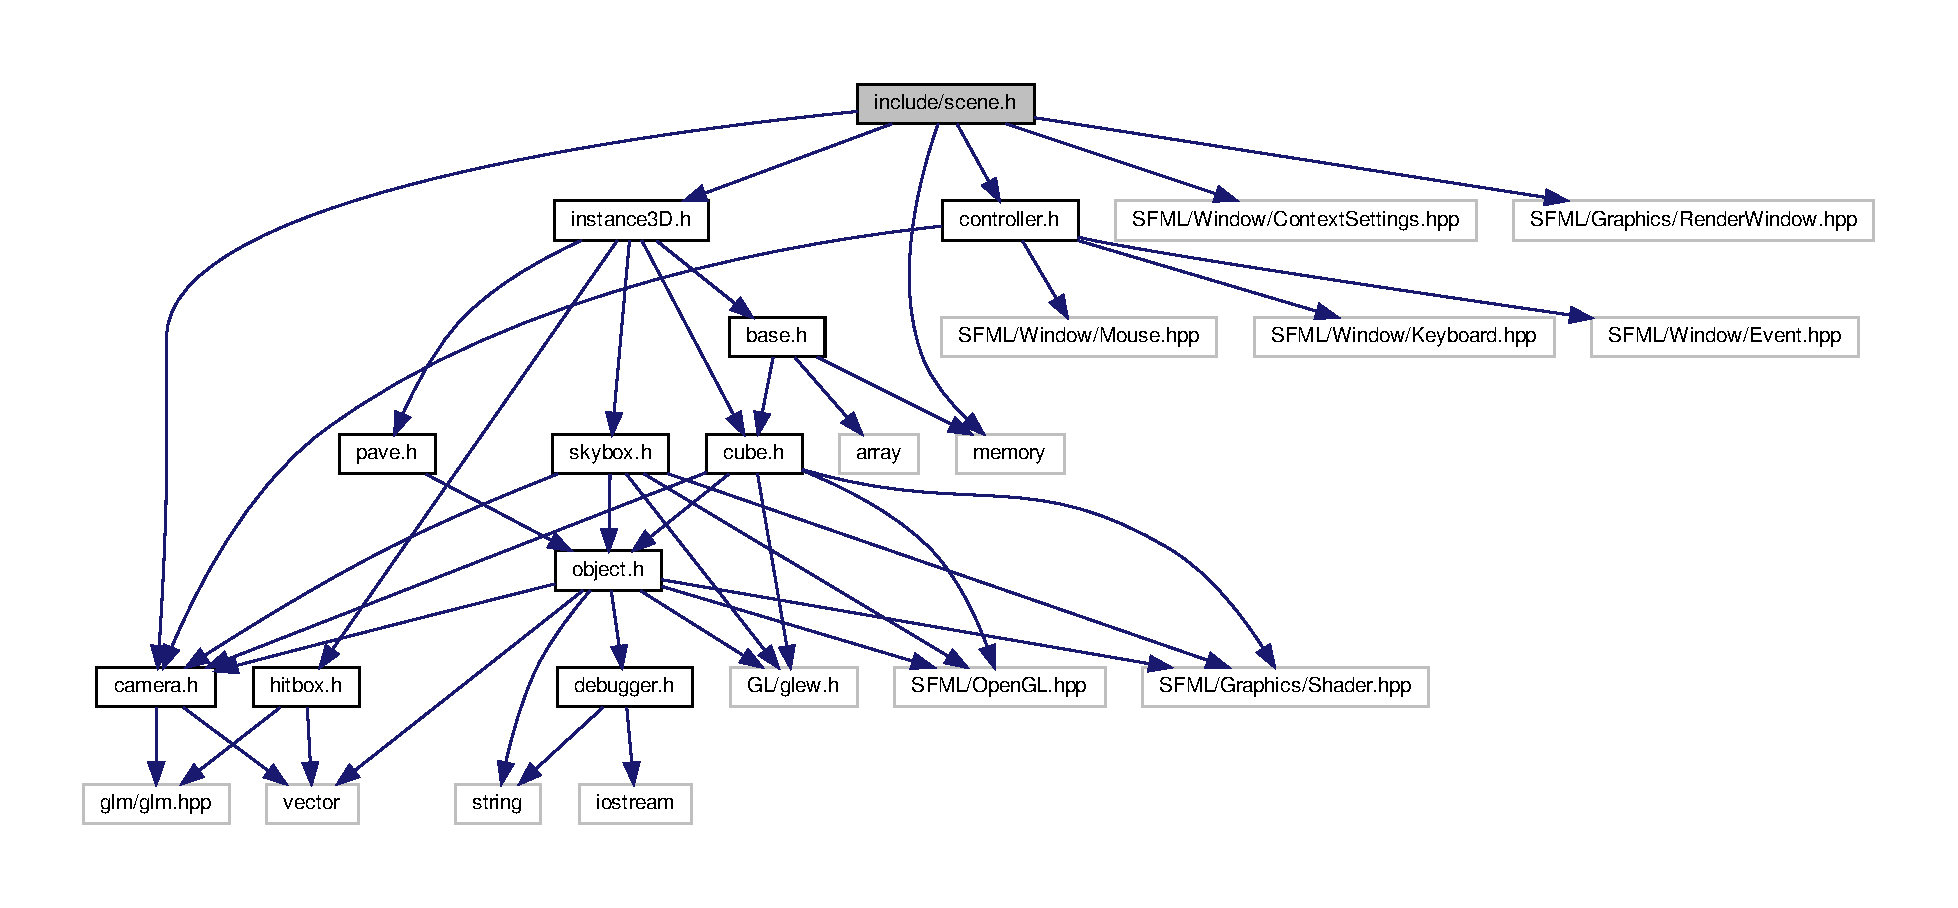
\includegraphics[width=350pt]{scene_8h__incl}
\end{center}
\end{figure}
This graph shows which files directly or indirectly include this file\+:\nopagebreak
\begin{figure}[H]
\begin{center}
\leavevmode
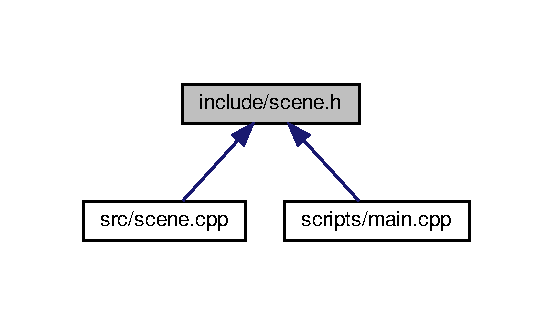
\includegraphics[width=266pt]{scene_8h__dep__incl}
\end{center}
\end{figure}
\subsection*{Classes}
\begin{DoxyCompactItemize}
\item 
class \hyperlink{classScene}{Scene}
\end{DoxyCompactItemize}

\hypertarget{skybox_8h}{}\section{include/skybox.h File Reference}
\label{skybox_8h}\index{include/skybox.\+h@{include/skybox.\+h}}
{\ttfamily \#include $<$camera.\+h$>$}\newline
{\ttfamily \#include $<$object.\+h$>$}\newline
{\ttfamily \#include $<$G\+L/glew.\+h$>$}\newline
{\ttfamily \#include $<$S\+F\+M\+L/\+Open\+G\+L.\+hpp$>$}\newline
{\ttfamily \#include $<$S\+F\+M\+L/\+Graphics/\+Shader.\+hpp$>$}\newline
Include dependency graph for skybox.\+h\+:\nopagebreak
\begin{figure}[H]
\begin{center}
\leavevmode
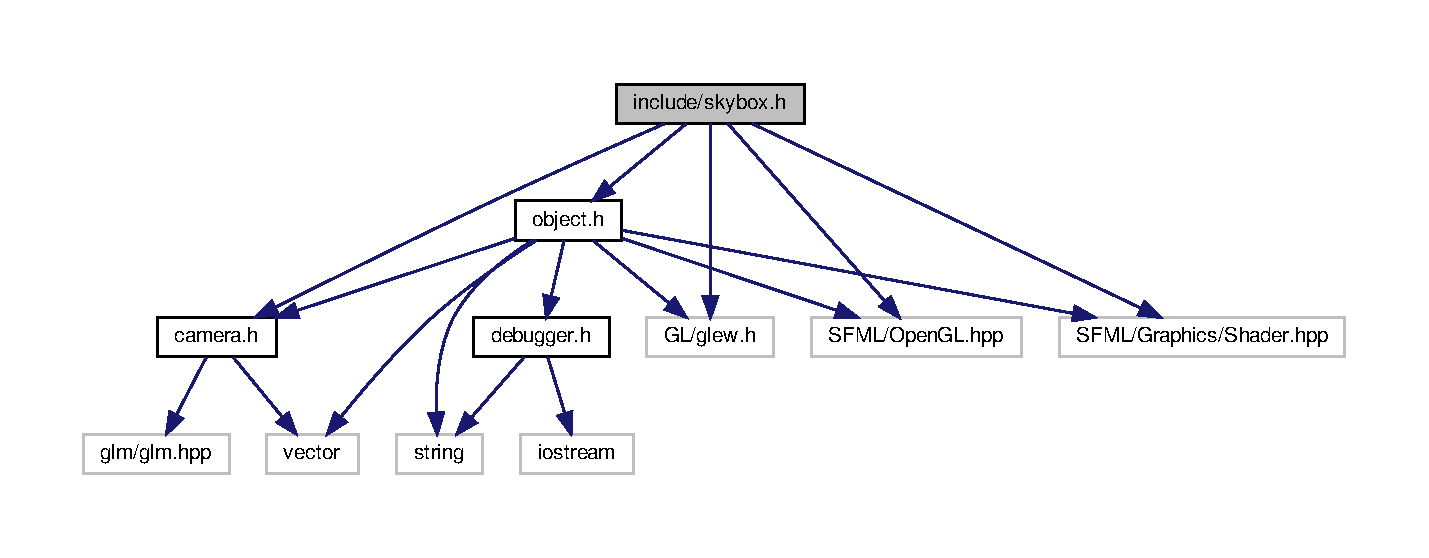
\includegraphics[width=350pt]{skybox_8h__incl}
\end{center}
\end{figure}
This graph shows which files directly or indirectly include this file\+:\nopagebreak
\begin{figure}[H]
\begin{center}
\leavevmode
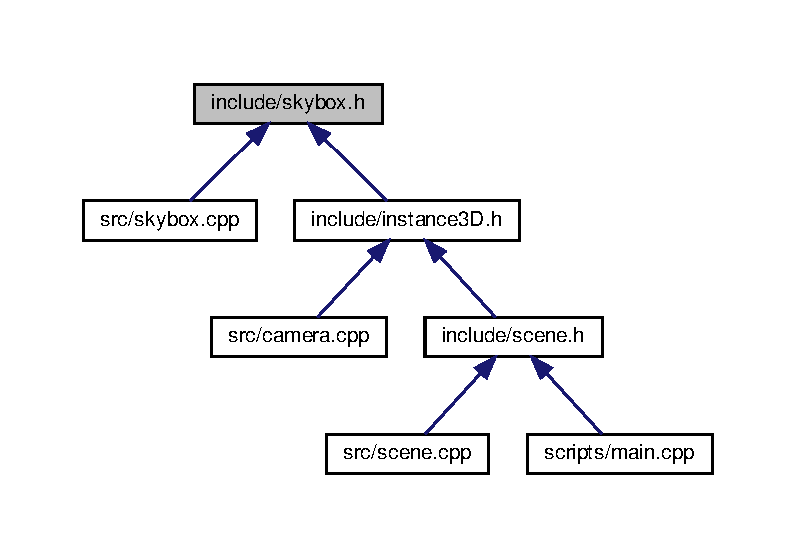
\includegraphics[width=350pt]{skybox_8h__dep__incl}
\end{center}
\end{figure}
\subsection*{Classes}
\begin{DoxyCompactItemize}
\item 
class \hyperlink{classSkybox}{Skybox}
\end{DoxyCompactItemize}

\hypertarget{main_8cpp}{}\section{scripts/main.cpp File Reference}
\label{main_8cpp}\index{scripts/main.\+cpp@{scripts/main.\+cpp}}
{\ttfamily \#include $<$scene.\+h$>$}\newline
Include dependency graph for main.\+cpp\+:\nopagebreak
\begin{figure}[H]
\begin{center}
\leavevmode
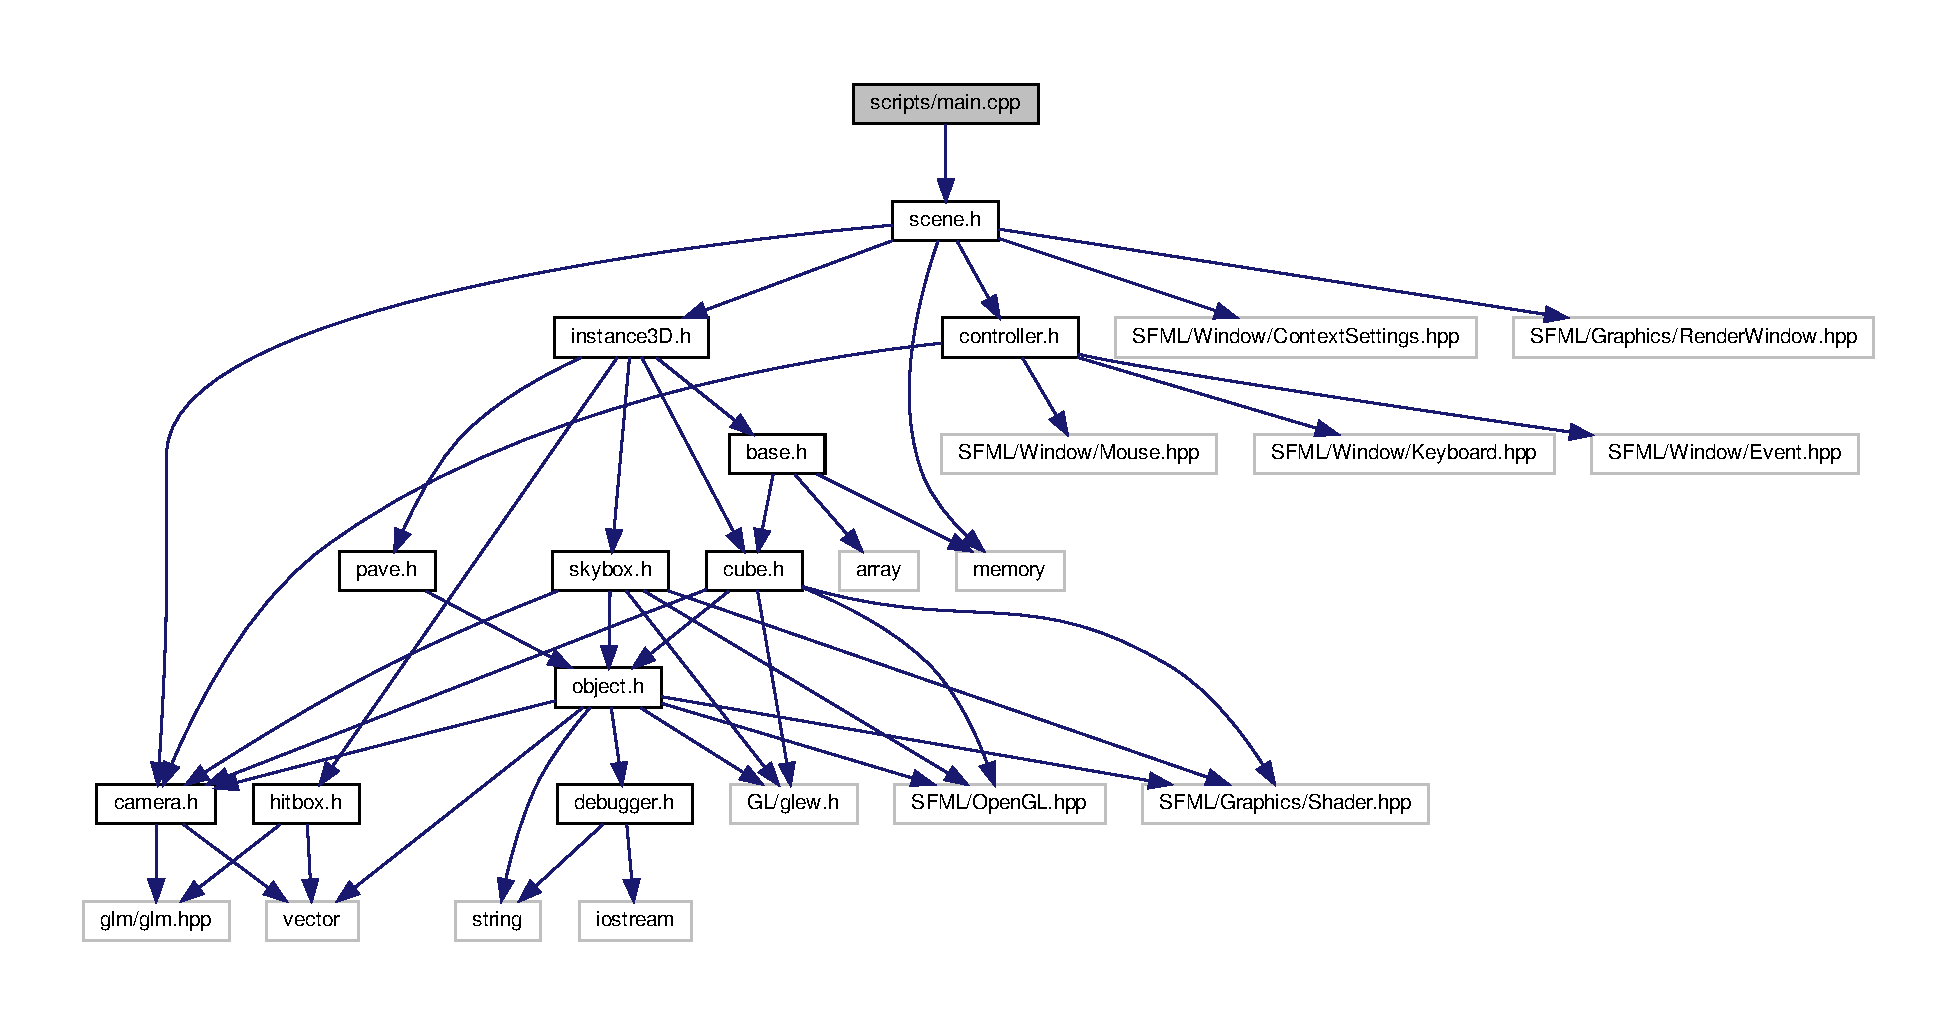
\includegraphics[width=350pt]{main_8cpp__incl}
\end{center}
\end{figure}
\subsection*{Functions}
\begin{DoxyCompactItemize}
\item 
int \hyperlink{main_8cpp_ae66f6b31b5ad750f1fe042a706a4e3d4}{main} ()
\end{DoxyCompactItemize}


\subsection{Function Documentation}
\mbox{\Hypertarget{main_8cpp_ae66f6b31b5ad750f1fe042a706a4e3d4}\label{main_8cpp_ae66f6b31b5ad750f1fe042a706a4e3d4}} 
\index{main.\+cpp@{main.\+cpp}!main@{main}}
\index{main@{main}!main.\+cpp@{main.\+cpp}}
\subsubsection{\texorpdfstring{main()}{main()}}
{\footnotesize\ttfamily int main (\begin{DoxyParamCaption}{ }\end{DoxyParamCaption})}


\hypertarget{base_8cpp}{}\section{src/base.cpp File Reference}
\label{base_8cpp}\index{src/base.\+cpp@{src/base.\+cpp}}
{\ttfamily \#include $<$base.\+h$>$}\newline
{\ttfamily \#include $<$glm/gtc/matrix\+\_\+transform.\+hpp$>$}\newline
Include dependency graph for base.\+cpp\+:\nopagebreak
\begin{figure}[H]
\begin{center}
\leavevmode
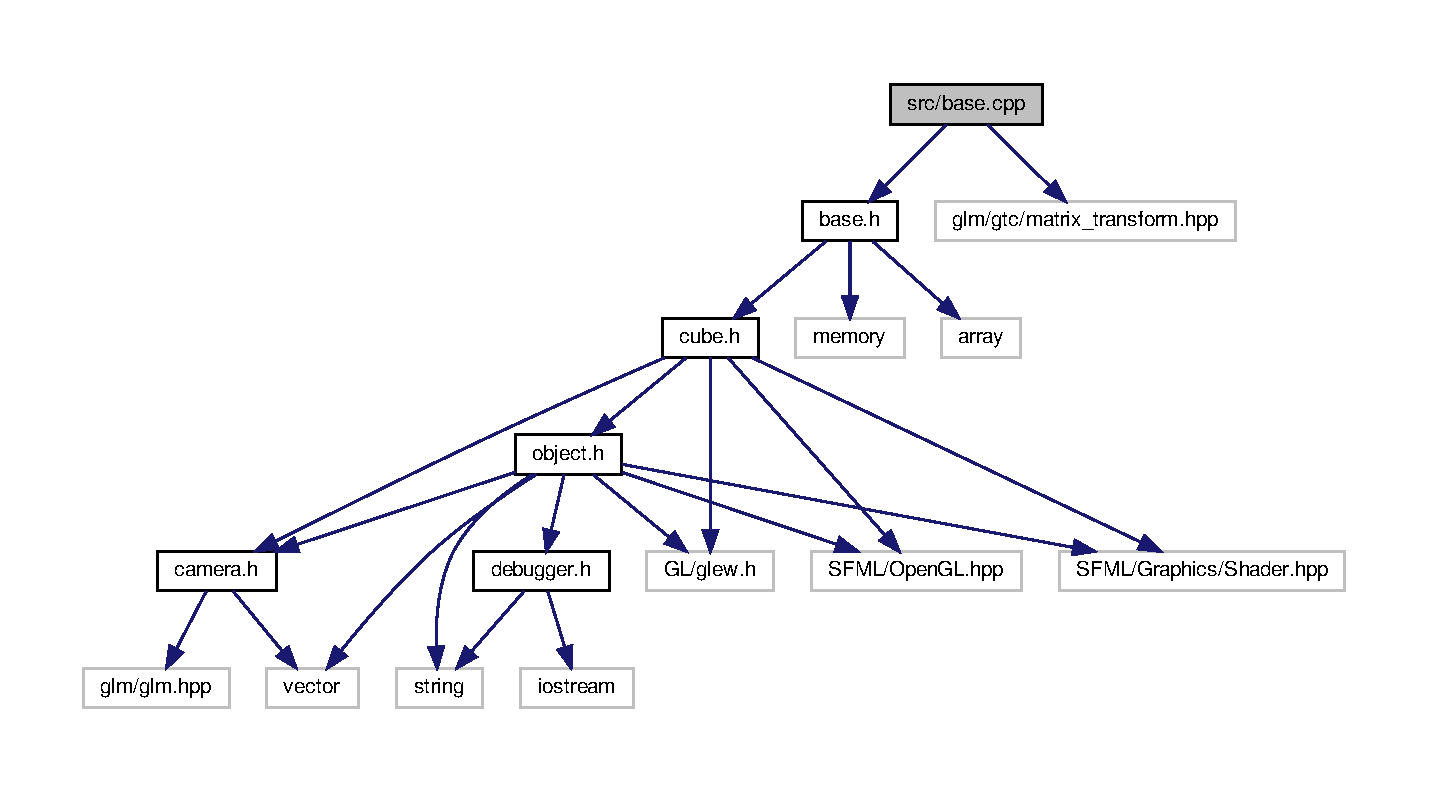
\includegraphics[width=350pt]{base_8cpp__incl}
\end{center}
\end{figure}
\subsection*{Variables}
\begin{DoxyCompactItemize}
\item 
constexpr float \hyperlink{base_8cpp_a165ec79ee9f2c8f79b0138da0c4b3ebd}{B\+A\+S\+E\+\_\+\+W\+I\+D\+TH} = 0.\+05f
\end{DoxyCompactItemize}


\subsection{Variable Documentation}
\mbox{\Hypertarget{base_8cpp_a165ec79ee9f2c8f79b0138da0c4b3ebd}\label{base_8cpp_a165ec79ee9f2c8f79b0138da0c4b3ebd}} 
\index{base.\+cpp@{base.\+cpp}!B\+A\+S\+E\+\_\+\+W\+I\+D\+TH@{B\+A\+S\+E\+\_\+\+W\+I\+D\+TH}}
\index{B\+A\+S\+E\+\_\+\+W\+I\+D\+TH@{B\+A\+S\+E\+\_\+\+W\+I\+D\+TH}!base.\+cpp@{base.\+cpp}}
\subsubsection{\texorpdfstring{B\+A\+S\+E\+\_\+\+W\+I\+D\+TH}{BASE\_WIDTH}}
{\footnotesize\ttfamily constexpr float B\+A\+S\+E\+\_\+\+W\+I\+D\+TH = 0.\+05f}


\hypertarget{camera_8cpp}{}\section{src/camera.cpp File Reference}
\label{camera_8cpp}\index{src/camera.\+cpp@{src/camera.\+cpp}}
{\ttfamily \#include $<$camera.\+h$>$}\newline
{\ttfamily \#include $<$instance3\+D.\+h$>$}\newline
{\ttfamily \#include $<$debugger.\+h$>$}\newline
{\ttfamily \#include $<$glm/gtc/matrix\+\_\+transform.\+hpp$>$}\newline
Include dependency graph for camera.\+cpp\+:\nopagebreak
\begin{figure}[H]
\begin{center}
\leavevmode
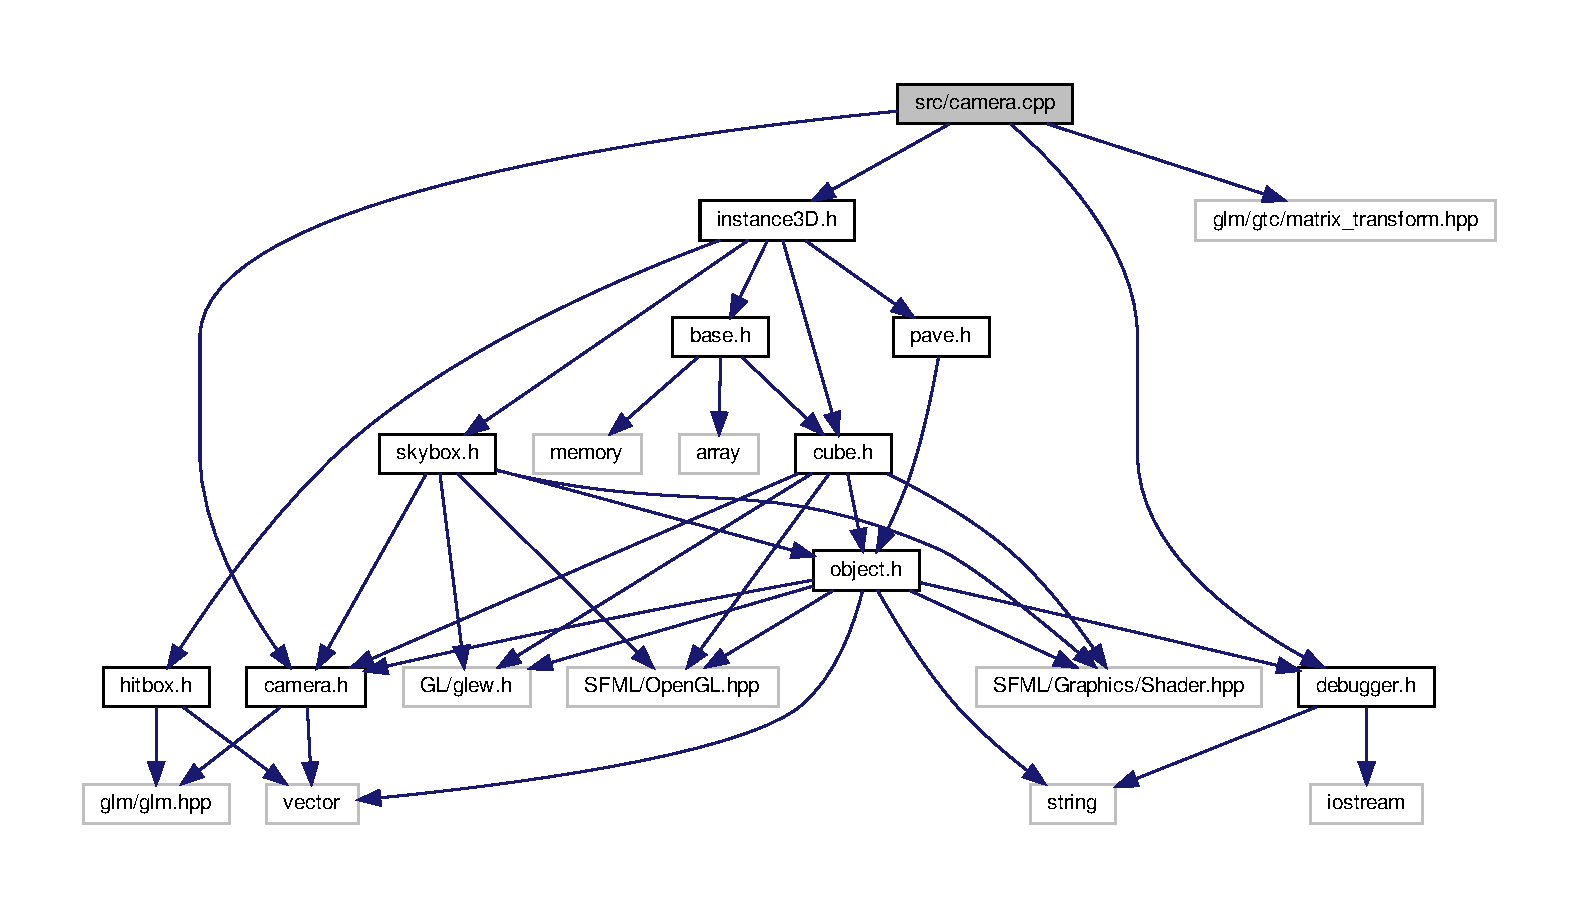
\includegraphics[width=350pt]{camera_8cpp__incl}
\end{center}
\end{figure}

\hypertarget{controller_8cpp}{}\section{src/controller.cpp File Reference}
\label{controller_8cpp}\index{src/controller.\+cpp@{src/controller.\+cpp}}
{\ttfamily \#include $<$controller.\+h$>$}\newline
Include dependency graph for controller.\+cpp\+:\nopagebreak
\begin{figure}[H]
\begin{center}
\leavevmode
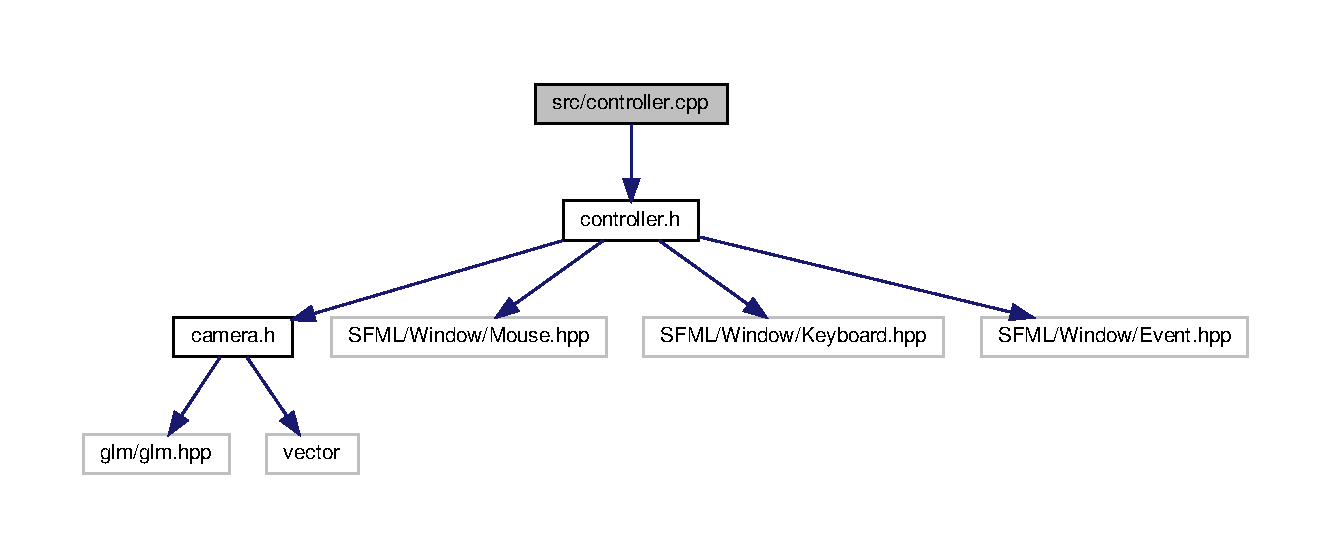
\includegraphics[width=350pt]{controller_8cpp__incl}
\end{center}
\end{figure}

\hypertarget{cube_8cpp}{}\section{src/cube.cpp File Reference}
\label{cube_8cpp}\index{src/cube.\+cpp@{src/cube.\+cpp}}
{\ttfamily \#include $<$cube.\+h$>$}\newline
{\ttfamily \#include $<$glm/gtc/type\+\_\+ptr.\+hpp$>$}\newline
{\ttfamily \#include $<$glm/gtc/matrix\+\_\+transform.\+hpp$>$}\newline
{\ttfamily \#include $<$S\+F\+M\+L/\+Graphics/\+Glsl.\+hpp$>$}\newline
{\ttfamily \#include $<$S\+F\+M\+L/\+Graphics/\+Image.\+hpp$>$}\newline
{\ttfamily \#include $<$iostream$>$}\newline
Include dependency graph for cube.\+cpp\+:\nopagebreak
\begin{figure}[H]
\begin{center}
\leavevmode
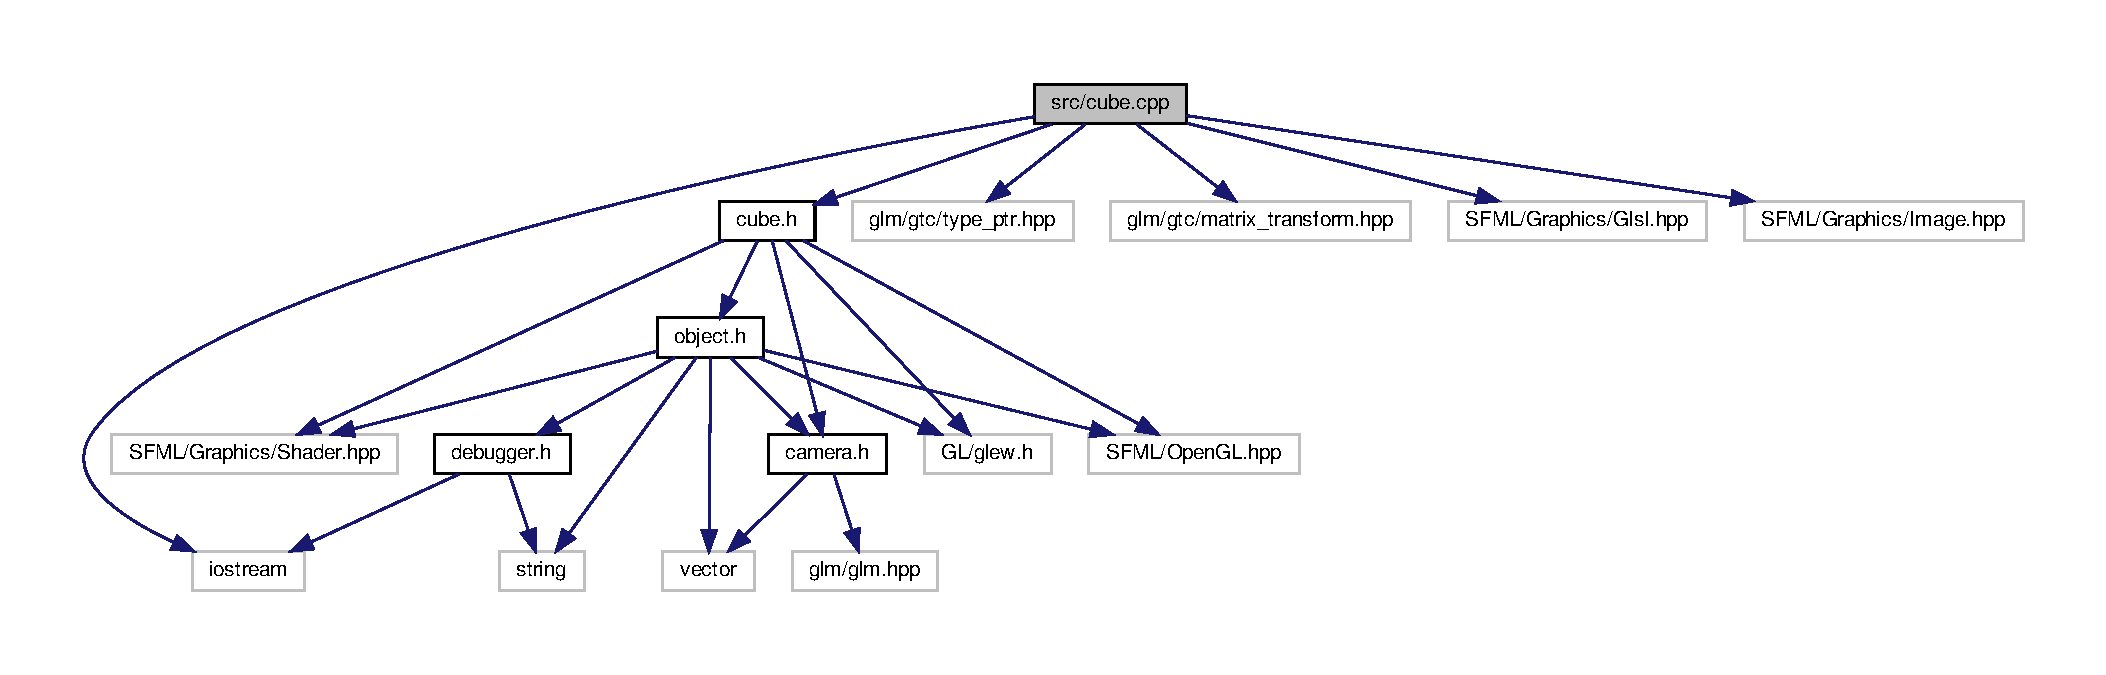
\includegraphics[width=350pt]{cube_8cpp__incl}
\end{center}
\end{figure}
\subsection*{Variables}
\begin{DoxyCompactItemize}
\item 
constexpr float \hyperlink{cube_8cpp_a4d3732b41dce829f776b7481166d5fcb}{S\+I\+ZE} = 1.\+0f
\item 
constexpr float \hyperlink{cube_8cpp_a8008b8187ef2958b055f5f35f892ab1b}{T\+E\+XT} = 1.\+0f
\item 
std\+::vector$<$ float $>$ \hyperlink{cube_8cpp_a87620882d99d672eca278bc9050e8fe8}{V\+E\+R\+T\+I\+C\+E\+S\+\_\+\+C\+U\+BE}
\end{DoxyCompactItemize}


\subsection{Variable Documentation}
\mbox{\Hypertarget{cube_8cpp_a4d3732b41dce829f776b7481166d5fcb}\label{cube_8cpp_a4d3732b41dce829f776b7481166d5fcb}} 
\index{cube.\+cpp@{cube.\+cpp}!S\+I\+ZE@{S\+I\+ZE}}
\index{S\+I\+ZE@{S\+I\+ZE}!cube.\+cpp@{cube.\+cpp}}
\subsubsection{\texorpdfstring{S\+I\+ZE}{SIZE}}
{\footnotesize\ttfamily constexpr float S\+I\+ZE = 1.\+0f}

\mbox{\Hypertarget{cube_8cpp_a8008b8187ef2958b055f5f35f892ab1b}\label{cube_8cpp_a8008b8187ef2958b055f5f35f892ab1b}} 
\index{cube.\+cpp@{cube.\+cpp}!T\+E\+XT@{T\+E\+XT}}
\index{T\+E\+XT@{T\+E\+XT}!cube.\+cpp@{cube.\+cpp}}
\subsubsection{\texorpdfstring{T\+E\+XT}{TEXT}}
{\footnotesize\ttfamily constexpr float T\+E\+XT = 1.\+0f}

\mbox{\Hypertarget{cube_8cpp_a87620882d99d672eca278bc9050e8fe8}\label{cube_8cpp_a87620882d99d672eca278bc9050e8fe8}} 
\index{cube.\+cpp@{cube.\+cpp}!V\+E\+R\+T\+I\+C\+E\+S\+\_\+\+C\+U\+BE@{V\+E\+R\+T\+I\+C\+E\+S\+\_\+\+C\+U\+BE}}
\index{V\+E\+R\+T\+I\+C\+E\+S\+\_\+\+C\+U\+BE@{V\+E\+R\+T\+I\+C\+E\+S\+\_\+\+C\+U\+BE}!cube.\+cpp@{cube.\+cpp}}
\subsubsection{\texorpdfstring{V\+E\+R\+T\+I\+C\+E\+S\+\_\+\+C\+U\+BE}{VERTICES\_CUBE}}
{\footnotesize\ttfamily std\+::vector$<$float$>$ V\+E\+R\+T\+I\+C\+E\+S\+\_\+\+C\+U\+BE}


\hypertarget{hitbox_8cpp}{}\section{src/hitbox.cpp File Reference}
\label{hitbox_8cpp}\index{src/hitbox.\+cpp@{src/hitbox.\+cpp}}
{\ttfamily \#include $<$hitbox.\+h$>$}\newline
Include dependency graph for hitbox.\+cpp\+:\nopagebreak
\begin{figure}[H]
\begin{center}
\leavevmode
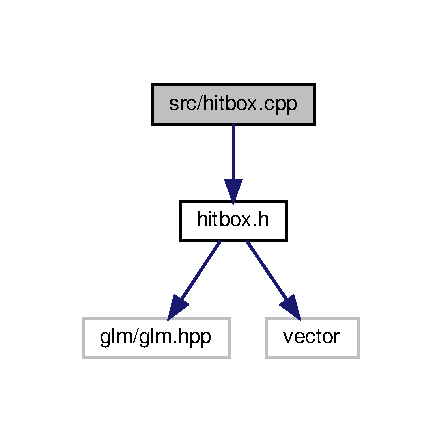
\includegraphics[width=212pt]{hitbox_8cpp__incl}
\end{center}
\end{figure}
\subsection*{Variables}
\begin{DoxyCompactItemize}
\item 
const std\+::vector$<$ glm\+::vec3 $>$ \hyperlink{hitbox_8cpp_aa48692978b2403900813b6ad0160ad6f}{N\+O\+R\+M\+A\+L\+\_\+\+V\+E\+C\+T\+O\+RS}
\end{DoxyCompactItemize}


\subsection{Variable Documentation}
\mbox{\Hypertarget{hitbox_8cpp_aa48692978b2403900813b6ad0160ad6f}\label{hitbox_8cpp_aa48692978b2403900813b6ad0160ad6f}} 
\index{hitbox.\+cpp@{hitbox.\+cpp}!N\+O\+R\+M\+A\+L\+\_\+\+V\+E\+C\+T\+O\+RS@{N\+O\+R\+M\+A\+L\+\_\+\+V\+E\+C\+T\+O\+RS}}
\index{N\+O\+R\+M\+A\+L\+\_\+\+V\+E\+C\+T\+O\+RS@{N\+O\+R\+M\+A\+L\+\_\+\+V\+E\+C\+T\+O\+RS}!hitbox.\+cpp@{hitbox.\+cpp}}
\subsubsection{\texorpdfstring{N\+O\+R\+M\+A\+L\+\_\+\+V\+E\+C\+T\+O\+RS}{NORMAL\_VECTORS}}
{\footnotesize\ttfamily const std\+::vector$<$glm\+::vec3$>$ N\+O\+R\+M\+A\+L\+\_\+\+V\+E\+C\+T\+O\+RS}

{\bfseries Initial value\+:}
\begin{DoxyCode}
\{
    glm::vec3( 1.0f,  0.0f,  0.0f),
    glm::vec3(-1.0f,  0.0f,  0.0f),
    glm::vec3( 0.0f,  1.0f,  0.0f),
    glm::vec3( 0.0f, -1.0f,  0.0f),
    glm::vec3( 0.0f,  0.0f,  1.0f),
    glm::vec3( 0.0f,  0.0f, -1.0f)
\}
\end{DoxyCode}

\hypertarget{pave_8cpp}{}\section{src/pave.cpp File Reference}
\label{pave_8cpp}\index{src/pave.\+cpp@{src/pave.\+cpp}}
{\ttfamily \#include $<$pave.\+h$>$}\newline
{\ttfamily \#include $<$glm/gtc/type\+\_\+ptr.\+hpp$>$}\newline
{\ttfamily \#include $<$glm/gtc/matrix\+\_\+transform.\+hpp$>$}\newline
{\ttfamily \#include $<$S\+F\+M\+L/\+Graphics/\+Glsl.\+hpp$>$}\newline
{\ttfamily \#include $<$S\+F\+M\+L/\+Graphics/\+Image.\+hpp$>$}\newline
{\ttfamily \#include $<$iostream$>$}\newline
Include dependency graph for pave.\+cpp\+:\nopagebreak
\begin{figure}[H]
\begin{center}
\leavevmode
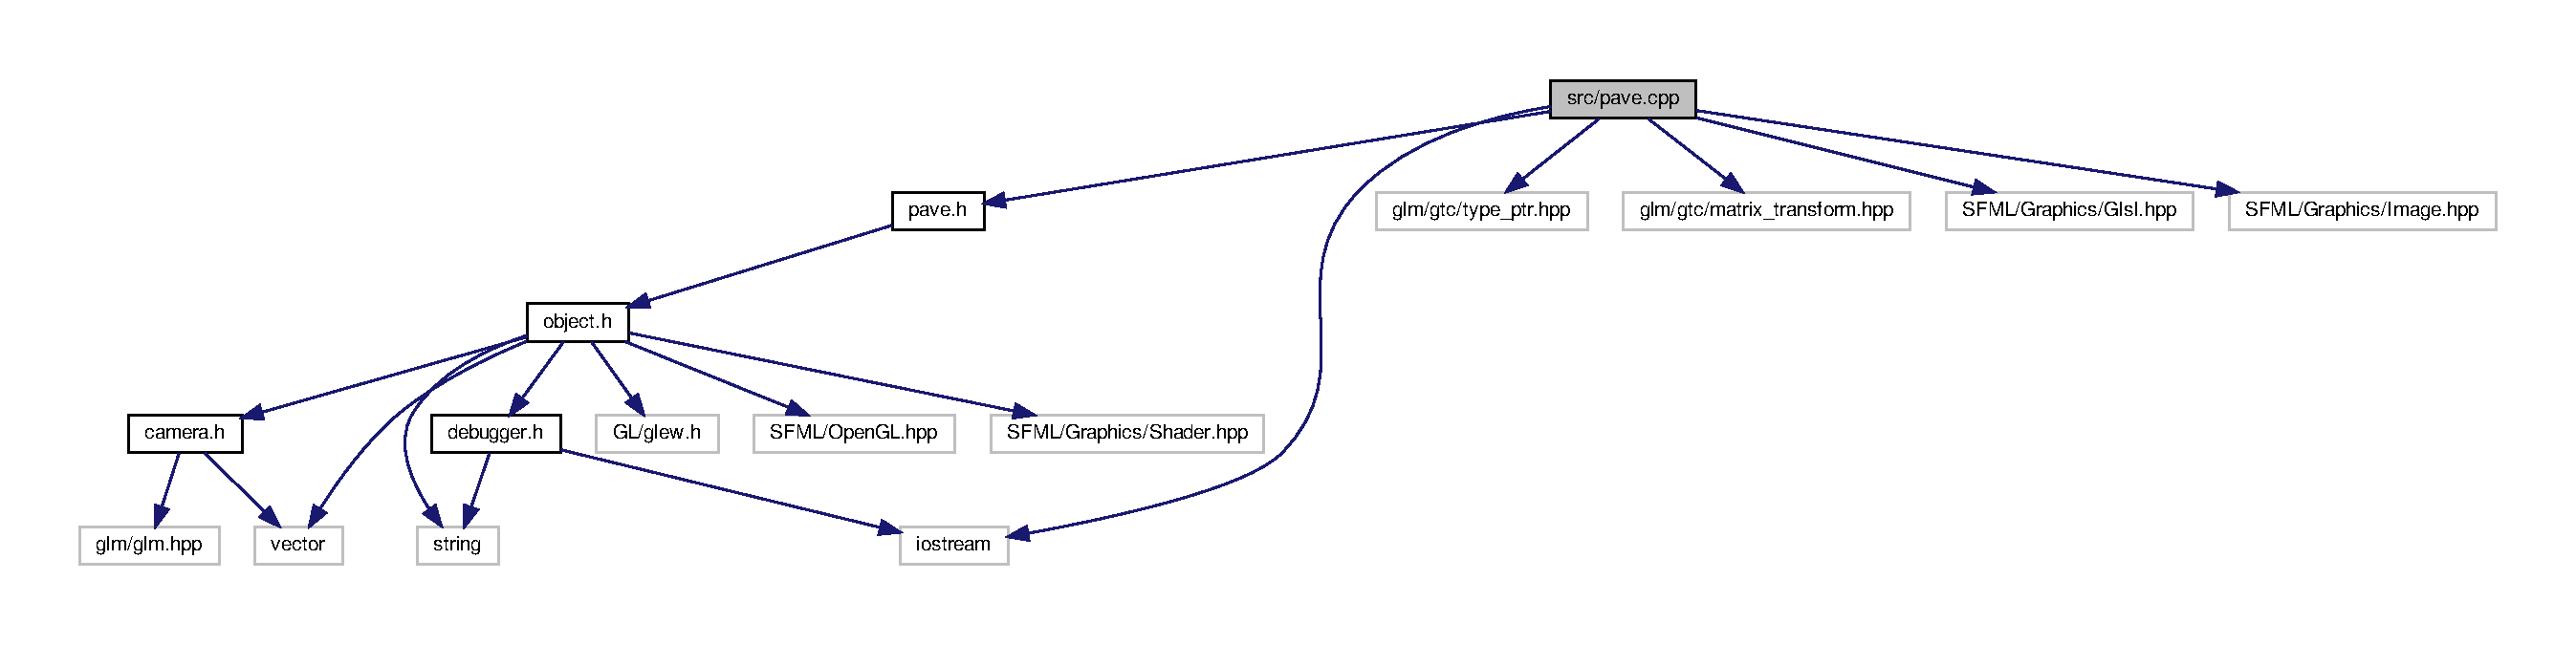
\includegraphics[width=350pt]{pave_8cpp__incl}
\end{center}
\end{figure}
\subsection*{Variables}
\begin{DoxyCompactItemize}
\item 
constexpr float \hyperlink{pave_8cpp_a7d3b76056fb64ecff3f31e9c8f7da450}{P\+A\+V\+E\+\_\+\+S\+I\+ZE} = 100
\item 
constexpr float \hyperlink{pave_8cpp_a8008b8187ef2958b055f5f35f892ab1b}{T\+E\+XT} = \hyperlink{pave_8cpp_a7d3b76056fb64ecff3f31e9c8f7da450}{P\+A\+V\+E\+\_\+\+S\+I\+ZE}
\item 
std\+::vector$<$ float $>$ \hyperlink{pave_8cpp_a9d56013e77711d5bbb446d481f60a8b3}{V\+E\+R\+T\+I\+C\+E\+S\+\_\+\+P\+A\+VE}
\end{DoxyCompactItemize}


\subsection{Variable Documentation}
\mbox{\Hypertarget{pave_8cpp_a7d3b76056fb64ecff3f31e9c8f7da450}\label{pave_8cpp_a7d3b76056fb64ecff3f31e9c8f7da450}} 
\index{pave.\+cpp@{pave.\+cpp}!P\+A\+V\+E\+\_\+\+S\+I\+ZE@{P\+A\+V\+E\+\_\+\+S\+I\+ZE}}
\index{P\+A\+V\+E\+\_\+\+S\+I\+ZE@{P\+A\+V\+E\+\_\+\+S\+I\+ZE}!pave.\+cpp@{pave.\+cpp}}
\subsubsection{\texorpdfstring{P\+A\+V\+E\+\_\+\+S\+I\+ZE}{PAVE\_SIZE}}
{\footnotesize\ttfamily constexpr float P\+A\+V\+E\+\_\+\+S\+I\+ZE = 100}

\mbox{\Hypertarget{pave_8cpp_a8008b8187ef2958b055f5f35f892ab1b}\label{pave_8cpp_a8008b8187ef2958b055f5f35f892ab1b}} 
\index{pave.\+cpp@{pave.\+cpp}!T\+E\+XT@{T\+E\+XT}}
\index{T\+E\+XT@{T\+E\+XT}!pave.\+cpp@{pave.\+cpp}}
\subsubsection{\texorpdfstring{T\+E\+XT}{TEXT}}
{\footnotesize\ttfamily constexpr float T\+E\+XT = \hyperlink{pave_8cpp_a7d3b76056fb64ecff3f31e9c8f7da450}{P\+A\+V\+E\+\_\+\+S\+I\+ZE}}

\mbox{\Hypertarget{pave_8cpp_a9d56013e77711d5bbb446d481f60a8b3}\label{pave_8cpp_a9d56013e77711d5bbb446d481f60a8b3}} 
\index{pave.\+cpp@{pave.\+cpp}!V\+E\+R\+T\+I\+C\+E\+S\+\_\+\+P\+A\+VE@{V\+E\+R\+T\+I\+C\+E\+S\+\_\+\+P\+A\+VE}}
\index{V\+E\+R\+T\+I\+C\+E\+S\+\_\+\+P\+A\+VE@{V\+E\+R\+T\+I\+C\+E\+S\+\_\+\+P\+A\+VE}!pave.\+cpp@{pave.\+cpp}}
\subsubsection{\texorpdfstring{V\+E\+R\+T\+I\+C\+E\+S\+\_\+\+P\+A\+VE}{VERTICES\_PAVE}}
{\footnotesize\ttfamily std\+::vector$<$float$>$ V\+E\+R\+T\+I\+C\+E\+S\+\_\+\+P\+A\+VE}

{\bfseries Initial value\+:}
\begin{DoxyCode}
\{    
        -\hyperlink{pave_8cpp_a7d3b76056fb64ecff3f31e9c8f7da450}{PAVE\_SIZE},  0.0f, -\hyperlink{pave_8cpp_a7d3b76056fb64ecff3f31e9c8f7da450}{PAVE\_SIZE},  0.0f, \hyperlink{pave_8cpp_a8008b8187ef2958b055f5f35f892ab1b}{TEXT},
         \hyperlink{pave_8cpp_a7d3b76056fb64ecff3f31e9c8f7da450}{PAVE\_SIZE},  0.0f, -\hyperlink{pave_8cpp_a7d3b76056fb64ecff3f31e9c8f7da450}{PAVE\_SIZE},  \hyperlink{pave_8cpp_a8008b8187ef2958b055f5f35f892ab1b}{TEXT}, \hyperlink{pave_8cpp_a8008b8187ef2958b055f5f35f892ab1b}{TEXT},
         \hyperlink{pave_8cpp_a7d3b76056fb64ecff3f31e9c8f7da450}{PAVE\_SIZE},  0.0f,  \hyperlink{pave_8cpp_a7d3b76056fb64ecff3f31e9c8f7da450}{PAVE\_SIZE},  \hyperlink{pave_8cpp_a8008b8187ef2958b055f5f35f892ab1b}{TEXT}, 0.0f,
         \hyperlink{pave_8cpp_a7d3b76056fb64ecff3f31e9c8f7da450}{PAVE\_SIZE},  0.0f,  \hyperlink{pave_8cpp_a7d3b76056fb64ecff3f31e9c8f7da450}{PAVE\_SIZE},  \hyperlink{pave_8cpp_a8008b8187ef2958b055f5f35f892ab1b}{TEXT}, 0.0f,
        -\hyperlink{pave_8cpp_a7d3b76056fb64ecff3f31e9c8f7da450}{PAVE\_SIZE},  0.0f,  \hyperlink{pave_8cpp_a7d3b76056fb64ecff3f31e9c8f7da450}{PAVE\_SIZE},  0.0f, 0.0f,
        -\hyperlink{pave_8cpp_a7d3b76056fb64ecff3f31e9c8f7da450}{PAVE\_SIZE},  0.0f, -\hyperlink{pave_8cpp_a7d3b76056fb64ecff3f31e9c8f7da450}{PAVE\_SIZE},  0.0f, \hyperlink{pave_8cpp_a8008b8187ef2958b055f5f35f892ab1b}{TEXT},
\}
\end{DoxyCode}

\hypertarget{scene_8cpp}{}\section{src/scene.cpp File Reference}
\label{scene_8cpp}\index{src/scene.\+cpp@{src/scene.\+cpp}}
{\ttfamily \#include $<$scene.\+h$>$}\newline
{\ttfamily \#include $<$debugger.\+h$>$}\newline
{\ttfamily \#include $<$glm/gtc/matrix\+\_\+transform.\+hpp$>$}\newline
{\ttfamily \#include $<$S\+F\+M\+L/\+Graphics.\+hpp$>$}\newline
{\ttfamily \#include $<$iostream$>$}\newline
Include dependency graph for scene.\+cpp\+:\nopagebreak
\begin{figure}[H]
\begin{center}
\leavevmode
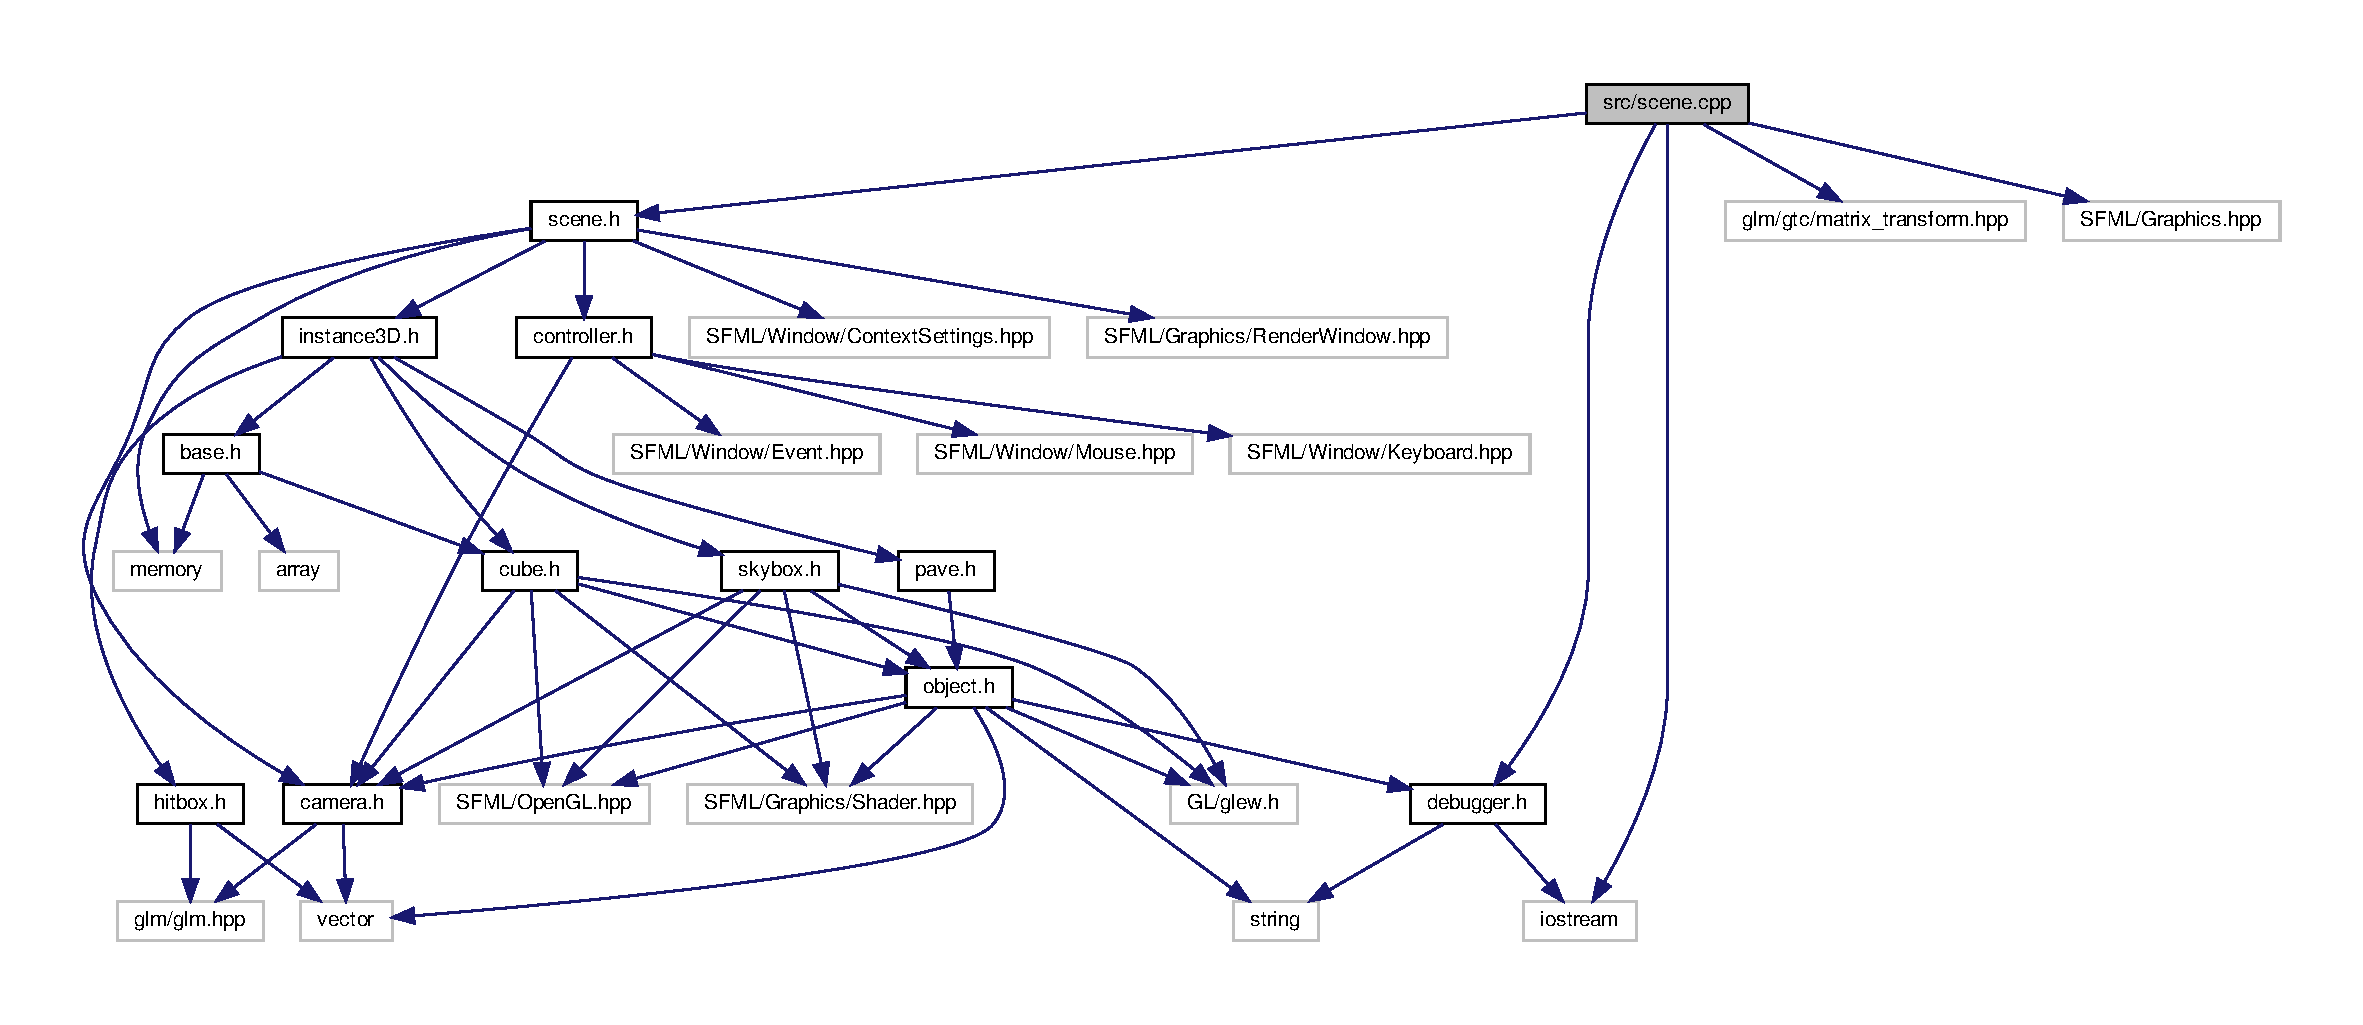
\includegraphics[width=350pt]{scene_8cpp__incl}
\end{center}
\end{figure}
\subsection*{Variables}
\begin{DoxyCompactItemize}
\item 
unsigned int \hyperlink{scene_8cpp_ad9effd43217aebb56382d72aca4bde76}{W\+I\+D\+TH} = 1600
\item 
unsigned int \hyperlink{scene_8cpp_a1616202489a4e64656da568d06754a57}{H\+E\+I\+G\+HT} = 900
\item 
float \hyperlink{scene_8cpp_a4664c5d930c290e6f82141a070cbea46}{lastX} = \hyperlink{scene_8cpp_ad9effd43217aebb56382d72aca4bde76}{W\+I\+D\+TH} / 2.\+0f
\item 
float \hyperlink{scene_8cpp_a9d5b8dfd025caf1c0ed043132515f587}{lastY} = \hyperlink{scene_8cpp_a1616202489a4e64656da568d06754a57}{H\+E\+I\+G\+HT} / 2.\+0f
\item 
bool \hyperlink{scene_8cpp_ac21731ba101e28334c34543121caa841}{first\+Mouse} = true
\end{DoxyCompactItemize}


\subsection{Variable Documentation}
\mbox{\Hypertarget{scene_8cpp_ac21731ba101e28334c34543121caa841}\label{scene_8cpp_ac21731ba101e28334c34543121caa841}} 
\index{scene.\+cpp@{scene.\+cpp}!first\+Mouse@{first\+Mouse}}
\index{first\+Mouse@{first\+Mouse}!scene.\+cpp@{scene.\+cpp}}
\subsubsection{\texorpdfstring{first\+Mouse}{firstMouse}}
{\footnotesize\ttfamily bool first\+Mouse = true}

\mbox{\Hypertarget{scene_8cpp_a1616202489a4e64656da568d06754a57}\label{scene_8cpp_a1616202489a4e64656da568d06754a57}} 
\index{scene.\+cpp@{scene.\+cpp}!H\+E\+I\+G\+HT@{H\+E\+I\+G\+HT}}
\index{H\+E\+I\+G\+HT@{H\+E\+I\+G\+HT}!scene.\+cpp@{scene.\+cpp}}
\subsubsection{\texorpdfstring{H\+E\+I\+G\+HT}{HEIGHT}}
{\footnotesize\ttfamily unsigned int H\+E\+I\+G\+HT = 900}

\mbox{\Hypertarget{scene_8cpp_a4664c5d930c290e6f82141a070cbea46}\label{scene_8cpp_a4664c5d930c290e6f82141a070cbea46}} 
\index{scene.\+cpp@{scene.\+cpp}!lastX@{lastX}}
\index{lastX@{lastX}!scene.\+cpp@{scene.\+cpp}}
\subsubsection{\texorpdfstring{lastX}{lastX}}
{\footnotesize\ttfamily float lastX = \hyperlink{scene_8cpp_ad9effd43217aebb56382d72aca4bde76}{W\+I\+D\+TH} / 2.\+0f}

\mbox{\Hypertarget{scene_8cpp_a9d5b8dfd025caf1c0ed043132515f587}\label{scene_8cpp_a9d5b8dfd025caf1c0ed043132515f587}} 
\index{scene.\+cpp@{scene.\+cpp}!lastY@{lastY}}
\index{lastY@{lastY}!scene.\+cpp@{scene.\+cpp}}
\subsubsection{\texorpdfstring{lastY}{lastY}}
{\footnotesize\ttfamily float lastY = \hyperlink{scene_8cpp_a1616202489a4e64656da568d06754a57}{H\+E\+I\+G\+HT} / 2.\+0f}

\mbox{\Hypertarget{scene_8cpp_ad9effd43217aebb56382d72aca4bde76}\label{scene_8cpp_ad9effd43217aebb56382d72aca4bde76}} 
\index{scene.\+cpp@{scene.\+cpp}!W\+I\+D\+TH@{W\+I\+D\+TH}}
\index{W\+I\+D\+TH@{W\+I\+D\+TH}!scene.\+cpp@{scene.\+cpp}}
\subsubsection{\texorpdfstring{W\+I\+D\+TH}{WIDTH}}
{\footnotesize\ttfamily unsigned int W\+I\+D\+TH = 1600}


\hypertarget{skybox_8cpp}{}\section{src/skybox.cpp File Reference}
\label{skybox_8cpp}\index{src/skybox.\+cpp@{src/skybox.\+cpp}}
{\ttfamily \#include $<$skybox.\+h$>$}\newline
{\ttfamily \#include $<$glm/gtc/type\+\_\+ptr.\+hpp$>$}\newline
{\ttfamily \#include $<$S\+F\+M\+L/\+Graphics/\+Glsl.\+hpp$>$}\newline
{\ttfamily \#include $<$S\+F\+M\+L/\+Graphics/\+Image.\+hpp$>$}\newline
{\ttfamily \#include $<$iostream$>$}\newline
Include dependency graph for skybox.\+cpp\+:\nopagebreak
\begin{figure}[H]
\begin{center}
\leavevmode
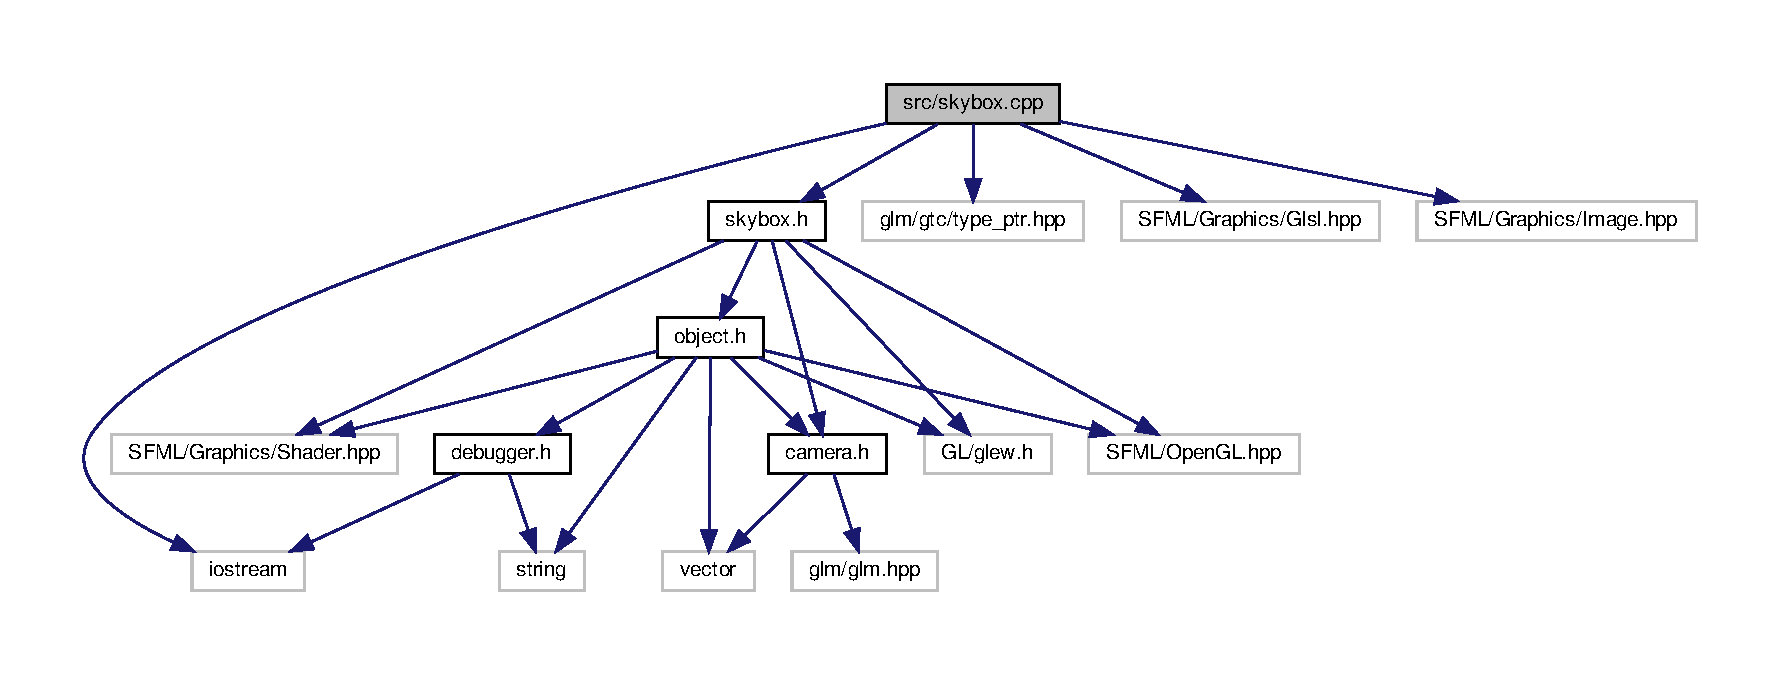
\includegraphics[width=350pt]{skybox_8cpp__incl}
\end{center}
\end{figure}
\subsection*{Variables}
\begin{DoxyCompactItemize}
\item 
constexpr float \hyperlink{skybox_8cpp_a4d3732b41dce829f776b7481166d5fcb}{S\+I\+ZE} = 0.\+5f
\item 
std\+::vector$<$ float $>$ \hyperlink{skybox_8cpp_a1e049e8451605c50cd2860c29a0250f1}{V\+E\+R\+T\+I\+C\+E\+S\+\_\+\+S\+K\+Y\+B\+OX}
\end{DoxyCompactItemize}


\subsection{Variable Documentation}
\mbox{\Hypertarget{skybox_8cpp_a4d3732b41dce829f776b7481166d5fcb}\label{skybox_8cpp_a4d3732b41dce829f776b7481166d5fcb}} 
\index{skybox.\+cpp@{skybox.\+cpp}!S\+I\+ZE@{S\+I\+ZE}}
\index{S\+I\+ZE@{S\+I\+ZE}!skybox.\+cpp@{skybox.\+cpp}}
\subsubsection{\texorpdfstring{S\+I\+ZE}{SIZE}}
{\footnotesize\ttfamily constexpr float S\+I\+ZE = 0.\+5f}

\mbox{\Hypertarget{skybox_8cpp_a1e049e8451605c50cd2860c29a0250f1}\label{skybox_8cpp_a1e049e8451605c50cd2860c29a0250f1}} 
\index{skybox.\+cpp@{skybox.\+cpp}!V\+E\+R\+T\+I\+C\+E\+S\+\_\+\+S\+K\+Y\+B\+OX@{V\+E\+R\+T\+I\+C\+E\+S\+\_\+\+S\+K\+Y\+B\+OX}}
\index{V\+E\+R\+T\+I\+C\+E\+S\+\_\+\+S\+K\+Y\+B\+OX@{V\+E\+R\+T\+I\+C\+E\+S\+\_\+\+S\+K\+Y\+B\+OX}!skybox.\+cpp@{skybox.\+cpp}}
\subsubsection{\texorpdfstring{V\+E\+R\+T\+I\+C\+E\+S\+\_\+\+S\+K\+Y\+B\+OX}{VERTICES\_SKYBOX}}
{\footnotesize\ttfamily std\+::vector$<$float$>$ V\+E\+R\+T\+I\+C\+E\+S\+\_\+\+S\+K\+Y\+B\+OX}


%--- End generated contents ---

% Index
\backmatter
\newpage
\phantomsection
\clearemptydoublepage
\addcontentsline{toc}{chapter}{Index}
\printindex

\end{document}
